\expandafter\ifx\csname MasterFile\endcsname\relax
\def\SubFile{hoge}
\documentclass[a4j,12pt,twoside,openany]{jreport}
%\nofiles %tocファイルを更新させない
%\documentclass[12pt,a4j,twoside,openany]{jsbook}
\usepackage[dvipdfmx]{graphicx}
\usepackage{../dspc} % ベースラインスキップの指定
\usepackage{../slashbox} % 表に斜線を入れる
%\usepackage{../mediabb}
\usepackage{fancyvrb} % Verbatim環境
\usepackage{fancyhdr} % Headerの下線付き章見出し
\usepackage{here} % float[H]
\usepackage{multirow}
\usepackage{hhline} % 表の罫線の角を美しくする
\usepackage{amsmath} %コレがないとcasesが動かない
\usepackage{amsfonts} % 数学用フォント
\usepackage{bm} % 数式環境での bold
\usepackage{algorithm}
\usepackage{algorithmicx}
\usepackage[noend]{algpseudocode}%\procedureはここに含まれる
\usepackage[flushleft]{threeparttable} % 脚注付きテーブル
\usepackage{enumitem}
\usepackage{comment}
\usepackage{fancybox}
%\usepackage{csvsimple,booktabs,siunitx}
%\usepackage{filecontents}
\usepackage{ulinej}


\setlength{\evensidemargin}{5pt}
\setlength{\oddsidemargin}{40pt}
%\setlength{\headheight}{16.5pt}
%%\setlength{\headheight}{30pt}
\setcounter{secnumdepth}{3}
\setlist[description]{leftmargin=2\parindent,labelindent=\parindent}

\makeatletter
\def\@makechapterhead#1{%
	\vspace*{50\p@}%
	{
		\parindent \z@ \raggedright \normalfont
		\ifnum \c@secnumdepth >\m@ne
		% \if@mainmatter
			\huge\bfseries\@chapapp\thechapter\@chappos
			\par\nobreak
			\vskip 20\p@
		% \fi
		\fi
		\interlinepenalty\@M
		\Huge\bfseries #1\par\nobreak
		\vskip 40\p@
	}
}

%新しいコマンド定義
\newcounter{linenumber}
\newenvironment{listing}{%
  \begin{list}{%
    \small\arabic{linenumber}:}{%
      \usecounter{linenumber}%
      \setlength{\baselineskip}{18pt}%
      \setlength{\itemsep}{0pt}%
      \setlength{\parsep}{0pt}}}%
 {\end{list}}
\newcommand{\figcaption}[1]{\def\@captype{figure}\caption{#1}}
\newcommand{\tblcaption}[1]{\def\@captype{table}\caption{#1}}
\newcommand{\norm}[1]{\left\| #1 \right\|}
\newcommand{\cc}[1]{\multicolumn{1}{|c|}{#1}}
\newcommand{\circled}[1]{\raisebox{.5pt}{\textcircled{\raisebox{-.9pt} {#1}}}}
\newcommand{\specialcell}[2][c]{%
  \begin{tabular}[#1]{@{}c@{}}#2\end{tabular}}
\makeatother
%===============================================================================
\expandafter\ifx\csname SubFile\endcsname\relax
\begin{document}
\def\MasterFile{hoge}
%-------------------------------------------------------------------------------
%\maketitle
\thispagestyle{empty}
\documentclass[a4j,12pt]{jarticle}
% 外表紙

% 題名
\def\title{降水量予測のための\\Sequence-to-Sequenceモデルに基づく\\マルチモーダル学習}
% 著者
\def\author{林 政行}
% 入学年度(平成)
\def\year{24}
% 学籍番号
\def\number{24115113}
% 指導教官
\def\kyoukan{伊藤孝行}
% 指導教官役職
\def\kyoukanrank{教授}
% 提出日
\def\teisyutubi{平成28年2月8日}

\begin{document}
\pagestyle{empty}
\baselineskip=18pt

\begin{center}

\vspace*{2cm}

{\huge \textbf{卒業論文}}

\vspace*{3cm}

%\vrule width 10cm height 1pt depth 0pt



%(題目)
%\vspace{5pt}
%\hrule height 3pt
%\vspace{1zh}

\vrule width 6.25cm height 6pt depth -2pt
\makebox[1.5cm]{(題目)}
\vrule width 6.25cm height 6pt depth -2pt

{\LARGE {\title}}

\vspace{1zh}
%{\large {\subtitle}}
%\hrule height 3pt
\vrule width 14cm height 4pt depth 0pt

\vspace*{1cm}

指導教員 {\large {\kyoukan}} {\kyoukanrank}

%\vspace*{5cm}
\vfill

{\large 名古屋工業大学 情報工学科}

{\large 平成{\year}年度 入学 ({\number})}

\vspace*{1cm}

%{\huge\mc {\author}}

\underline{(氏名)\hspace{3zw}{\huge\mc {\author}}\hspace{3zw}}

\vspace*{1cm}

({\teisyutubi}提出)

\vspace{2cm}
\end{center}

\end{document}
\begin{titlepage}

% 題名
\def\title{分散表現を用いた\\話題変化判定}
% 補助題名
\def\subtitle{卒業論文}
% 著者
\def\author{芳野 魁}
% 入学年度(平成)
\def\year{29}
% 学籍番号
\def\number{26115162}
% 指導教官
\def\kyoukan{伊藤 孝行}
% 指導教官役職
\def\kyoukanrank{教授}
% 提出日
\def\teisyutubi{平成29年9月19日}

\pagestyle{empty}

\begin{center}

\vspace*{20mm}
{\Large\mc 平成29年度 \hspace{7mm} 卒 業 論 文}
\vspace{15mm}

%\setlength{\unitlength}{1mm}
\begin{picture}(100,60)
  \put(0,0){\makebox(100,60){\huge\bf\shortstack{\title}}}
\end{picture}
\\
%\begin{picture}(100,5)
%  \put(0,0){\makebox(100,5){\Large\bf\shortstack{\subtitle}}}
%\end{picture}
\end{center}
\vspace{10mm}
\begin{flushright}
\begin{tabular}{ll}
{\large 提出日} & {\large {\teisyutubi}} \\
{\large 所属}  & {\large 名古屋工業大学 情報工学科} \\
{\large 指導教員} & {\large {\kyoukan} {\kyoukanrank}} \\
 & \\
{\large 入学年度} & {\large 平成{\year}年度入学}\\
{\large 学籍番号} &{\large {\number}} \\
 & \\
%{\large 氏名} & {\huge {\author}}
{\large 氏名} & {\huge\mc {\author}}
\end{tabular}
\end{flushright}

\end{titlepage}

%\addcontentsline{toc}{chapter}{表紙}
\thispagestyle{empty}
\mbox{}\newpage
%===============================================================================
%\frontmatter
%===============================================================================
%\mainmatter
%-------------------------------------------------------------------------------
\pagenumbering{arabic}
\cleardoublepage
\expandafter\ifx\csname MasterFile\endcsname\relax
\def\SubFile{hoge}
\documentclass[a4j,12pt,twoside,openany]{jreport}
%\nofiles %tocファイルを更新させない
%\documentclass[12pt,a4j,twoside,openany]{jsbook}
\usepackage[dvipdfmx]{graphicx}
\usepackage{../dspc} % ベースラインスキップの指定
\usepackage{../slashbox} % 表に斜線を入れる
%\usepackage{../mediabb}
\usepackage{fancyvrb} % Verbatim環境
\usepackage{fancyhdr} % Headerの下線付き章見出し
\usepackage{here} % float[H]
\usepackage{multirow}
\usepackage{hhline} % 表の罫線の角を美しくする
\usepackage{amsmath} %コレがないとcasesが動かない
\usepackage{amsfonts} % 数学用フォント
\usepackage{bm} % 数式環境での bold
\usepackage{algorithm}
\usepackage{algorithmicx}
\usepackage[noend]{algpseudocode}%\procedureはここに含まれる
\usepackage[flushleft]{threeparttable} % 脚注付きテーブル
\usepackage{enumitem}
\usepackage{comment}
\usepackage{fancybox}
%\usepackage{csvsimple,booktabs,siunitx}
%\usepackage{filecontents}
\usepackage{ulinej}


\setlength{\evensidemargin}{5pt}
\setlength{\oddsidemargin}{40pt}
%\setlength{\headheight}{16.5pt}
%%\setlength{\headheight}{30pt}
\setcounter{secnumdepth}{3}
\setlist[description]{leftmargin=2\parindent,labelindent=\parindent}

\makeatletter
\def\@makechapterhead#1{%
	\vspace*{50\p@}%
	{
		\parindent \z@ \raggedright \normalfont
		\ifnum \c@secnumdepth >\m@ne
		% \if@mainmatter
			\huge\bfseries\@chapapp\thechapter\@chappos
			\par\nobreak
			\vskip 20\p@
		% \fi
		\fi
		\interlinepenalty\@M
		\Huge\bfseries #1\par\nobreak
		\vskip 40\p@
	}
}

%新しいコマンド定義
\newcounter{linenumber}
\newenvironment{listing}{%
  \begin{list}{%
    \small\arabic{linenumber}:}{%
      \usecounter{linenumber}%
      \setlength{\baselineskip}{18pt}%
      \setlength{\itemsep}{0pt}%
      \setlength{\parsep}{0pt}}}%
 {\end{list}}
\newcommand{\figcaption}[1]{\def\@captype{figure}\caption{#1}}
\newcommand{\tblcaption}[1]{\def\@captype{table}\caption{#1}}
\newcommand{\norm}[1]{\left\| #1 \right\|}
\newcommand{\cc}[1]{\multicolumn{1}{|c|}{#1}}
\newcommand{\circled}[1]{\raisebox{.5pt}{\textcircled{\raisebox{-.9pt} {#1}}}}
\newcommand{\specialcell}[2][c]{%
  \begin{tabular}[#1]{@{}c@{}}#2\end{tabular}}
\makeatother
%===============================================================================
\expandafter\ifx\csname SubFile\endcsname\relax
\begin{document}
\def\MasterFile{hoge}
%-------------------------------------------------------------------------------
%\maketitle
\thispagestyle{empty}
\input{../hyoushi/hyoushi}
\input{../hyoushi/title}
%\addcontentsline{toc}{chapter}{表紙}
\thispagestyle{empty}
\mbox{}\newpage
%===============================================================================
%\frontmatter
%===============================================================================
%\mainmatter
%-------------------------------------------------------------------------------
\pagenumbering{arabic}
\cleardoublepage
\input{../0.Abstract/chapter}
%-------------------------------------------------------------------------------
\clearpage
\addcontentsline{toc}{chapter}{目次}
\tableofcontents

\clearpage
\addcontentsline{toc}{chapter}{図目次}
\listoffigures

\clearpage
\addcontentsline{toc}{chapter}{表目次}
\listoftables

%-------------------------------------------------------------------------------

%=====================
\pagestyle{fancy} % Headerをつける
\renewcommand{\sectionmark}[1]{\markright{\thesection\ \ \ #1}}
\renewcommand{\chaptermark}[1]{\markboth{#1}{}}
\lhead{}
\chead{}
\lfoot{}
\rfoot{}%-------------------------------------------------------------------------------
\input{../1.Introduction/chapter}
%-------------------------------------------------------------------------------
\input{../2.Related_Work/chapter}
%-------------------------------------------------------------------------------
\input{../3.The_Model/chapter}
%-------------------------------------------------------------------------------
\input{../4.Implementation/chapter}
%-------------------------------------------------------------------------------
\input{../5.Experiments/chapter}
%-------------------------------------------------------------------------------
\input{../6.Conclusion/chapter}

%===============================================================================
\pagestyle{plain}
%-------------------------------------------------------------------------------
\input{../7.Acknowledgement/chapter} %謝辞
%-------------------------------------------------------------------------------
\def\BibFile{../Bibliograhoy/database2}
\input{../Bibliography/chapter} %参考文献
% %===============================================================================
\appendix
\input{../A.Mypaper/chapter} % 投稿論文リスト
\input{../B.SIG-CCI2/chapter} %
\input{../C.IPSJ80/chapter} %
\input{../D.TopicGraph/chapter} %
%===============================================================================
\end{document}\input{../../../../../../../Downloads/2章.docx}

\fi

\begin{document}
\fi
%-------------------------------------------------------------------------------
\cleardoublepage
\chapter*{論文要旨}\addcontentsline{toc}{chapter}{論文要旨}
近年,Web上での大規模な議論活動が活発になっているが,現在一般的に使われている "2ちゃんねる" や "Twitter" といったシステムでは整理や収束を行うことが困難である.困難である原因として,議論の管理を行う者がいないことが挙げられる.
議論を収束させるには議論のマネジメントを行う人物が必要である.
%
大規模意見集約システムCOLLAGREEではファシリテーターと呼ばれる人物が議論のマネジメントを行っている.
しかし,ファシリテーターは人間であり,長時間に渡って大人数での議論の動向をマネジメントし続けるのは困難である.
%
COLLAGREEで大規模な議論を収束させるためには,ファシリテーターが必要な時にだけ画面を見るようにして画面に向き合う時間を減らす工夫があることが望ましい.ファシリテーターが画面を見るべきタイミングは議論の話題が変化したときである.以前の議論の内容から外れた発言がされた時,ファシリテーターが適切に発言することで,脱線や炎上を避けて議論を収束させることができる.
すなわち,ファシリテーターの代わりに自動的に議論中の話題の変化を事前に判定することが求められている.
%
現在,COLLAGREE上で使用されている議論支援システムは投稿支援システムと議論可視化システムの2つに大別できる.
投稿支援システムはポイント機能やファシリテーションフレーズ簡易投稿機能のように,ユーザーが投稿をする際に何らかの補助やリアクションを行う.現行の機能では選択肢の提示に留まっており,作業量を減らすことには繋がりにくい。
一方,議論可視化システムは議論ツリーやキーワード抽出のように,ユーザーにスレッドとは異なる議論の見方を提供する.現行の機能では議論を見やすくすることに重点が置かれており,議論の把握の助けにはなるが画面に向き合う時間を減らすことにはなりにくい.むしろ,作業量を増やすことになり得る機能もある.
\begin{comment}
ポイント機能(ユーザの議論行動を活性化)-1
ファシリテーションフレーズ簡易投稿機能-1
議論ツリー-2
1文の要約,スレッドの要約,クラスタリング,返信意見の極性判定-2
ファシリテーションスタンプ-1
キーワード抽出-2
いいね機能-1
いいねランキング-2
投票機能-1
議論フェーズ機能-2
1-意見を出す、投稿をする際に補助や選択肢、リアクションを与える
2-議論の別の見方を提供する
\end{comment}
%
近年,自然言語処理の分野において分散表現が多くの研究で使われており,機械翻訳を始めとする単語の意味が重要となる分野で精度の向上が確認されている.分散表現を用いることで,人間に近い精度で話題の変化を観測することが可能となる.
%
以上のような背景を踏まえて,分散表現を用いて,話題の変化を観測し,話題の変化が確認された時にファシリテーターに伝えることが望ましい.
話題の変化の観測は,発言中に現れる単語の関連度合いの計算と見なすことができる.
分散表現を用いることで単語間の類似度を求めることができる,値が大きいほど単語がそれぞれ類似した実数ベクトルであることを表す.単語Aと単語Bの実数ベクトルが類似しているとは,単語Aと共に使われることの多い単語と単語Bと共に使われることの多い単語が多く共通していることを示す.故に,分散表現を使って単語の関連度を計算することができる.
%
発言文から単語を選ぶ際には自動要約を用いる.発言文から重要でない単語を取り除くことで関連度の計算の精度を高めることが可能となる.
%
本論文では,分散表現を用いて議論中での発言に含まれる単語の関連度を計算し,話題の変化を観測する手法を提案する.
%
提案手法は,既存の抽出的要約手法を用いて選ばれた単語の関連度を計算する手法,Seq2Seqによる生成的要約を用いて生成された単語の関連度を計算する手法,オントロジーを用いて求められた単語の関連度を計算する手法の3つである.
提案した3つの手法により,議論中の話題の変化の観測の評価実験を行い,各手法の評価を行う.
評価実験によって,提案手法を用いることで人間の代わりに自動的に話題の変化を観測できることを確認する.
%
 \begin{comment}
大規模な議論では意見を共有することは可能であるが,議論を整理させることや収束させることは難しい.以上から大規模意見集約システムCOLLAGREEが開発された.本システムではWeb上で適切に大規模な議論を行うことができるように議論をマネジメントするファシリテーターを導入した.
過去の実験ではファシリテーターの存在が議論の集約に大きな役割を果たしていることが認識されており,大規模な議論のためにファシリテータは必要である.しかし,議論の規模に伴って議論時間が長くなる傾向があり,同時にファシリテーターは常に議論の動向を見続ける必要がある.故に,議論の規模が大きくなればなるほどファシリテーターは長時間かつ大規模な議論の動向の監視によって大きな負担がかかる.大規模な議論が増加する傾向を踏まえるとファシリテーターにかかる負担を軽減する支援が必要となることは明白である.
また,近年自然言語処理の分野において分散表現が多くの研究で使われており,機械翻訳を始めとする複数の分野で精度の向上が確認されている.まだ適応されていない分野でも結果の向上が期待できる.
従って,本研究では負担軽減の1つとして分散表現を用いて議論中での話題の変化を人間の代わりに検知することでファシリテーターの負担を軽減することを目指す.
-----------------

\end{comment}
%-------------------------------------------------------------------------------
\expandafter\ifx\csname MasterFile\endcsname\relax
\end{document}
\fi

%-------------------------------------------------------------------------------
\clearpage
\addcontentsline{toc}{chapter}{目次}
\tableofcontents

\clearpage
\addcontentsline{toc}{chapter}{図目次}
\listoffigures

\clearpage
\addcontentsline{toc}{chapter}{表目次}
\listoftables

%-------------------------------------------------------------------------------

%=====================
\pagestyle{fancy} % Headerをつける
\renewcommand{\sectionmark}[1]{\markright{\thesection\ \ \ #1}}
\renewcommand{\chaptermark}[1]{\markboth{#1}{}}
\lhead{}
\chead{}
\lfoot{}
\rfoot{}%-------------------------------------------------------------------------------
\expandafter\ifx\csname MasterFile\endcsname\relax
\def\SubFile{hoge}
\documentclass[a4j,12pt,twoside,openany]{jreport}
%\nofiles %tocファイルを更新させない
%\documentclass[12pt,a4j,twoside,openany]{jsbook}
\usepackage[dvipdfmx]{graphicx}
\usepackage{../dspc} % ベースラインスキップの指定
\usepackage{../slashbox} % 表に斜線を入れる
%\usepackage{../mediabb}
\usepackage{fancyvrb} % Verbatim環境
\usepackage{fancyhdr} % Headerの下線付き章見出し
\usepackage{here} % float[H]
\usepackage{multirow}
\usepackage{hhline} % 表の罫線の角を美しくする
\usepackage{amsmath} %コレがないとcasesが動かない
\usepackage{amsfonts} % 数学用フォント
\usepackage{bm} % 数式環境での bold
\usepackage{algorithm}
\usepackage{algorithmicx}
\usepackage[noend]{algpseudocode}%\procedureはここに含まれる
\usepackage[flushleft]{threeparttable} % 脚注付きテーブル
\usepackage{enumitem}
\usepackage{comment}
\usepackage{fancybox}
%\usepackage{csvsimple,booktabs,siunitx}
%\usepackage{filecontents}
\usepackage{ulinej}


\setlength{\evensidemargin}{5pt}
\setlength{\oddsidemargin}{40pt}
%\setlength{\headheight}{16.5pt}
%%\setlength{\headheight}{30pt}
\setcounter{secnumdepth}{3}
\setlist[description]{leftmargin=2\parindent,labelindent=\parindent}

\makeatletter
\def\@makechapterhead#1{%
	\vspace*{50\p@}%
	{
		\parindent \z@ \raggedright \normalfont
		\ifnum \c@secnumdepth >\m@ne
		% \if@mainmatter
			\huge\bfseries\@chapapp\thechapter\@chappos
			\par\nobreak
			\vskip 20\p@
		% \fi
		\fi
		\interlinepenalty\@M
		\Huge\bfseries #1\par\nobreak
		\vskip 40\p@
	}
}

%新しいコマンド定義
\newcounter{linenumber}
\newenvironment{listing}{%
  \begin{list}{%
    \small\arabic{linenumber}:}{%
      \usecounter{linenumber}%
      \setlength{\baselineskip}{18pt}%
      \setlength{\itemsep}{0pt}%
      \setlength{\parsep}{0pt}}}%
 {\end{list}}
\newcommand{\figcaption}[1]{\def\@captype{figure}\caption{#1}}
\newcommand{\tblcaption}[1]{\def\@captype{table}\caption{#1}}
\newcommand{\norm}[1]{\left\| #1 \right\|}
\newcommand{\cc}[1]{\multicolumn{1}{|c|}{#1}}
\newcommand{\circled}[1]{\raisebox{.5pt}{\textcircled{\raisebox{-.9pt} {#1}}}}
\newcommand{\specialcell}[2][c]{%
  \begin{tabular}[#1]{@{}c@{}}#2\end{tabular}}
\makeatother
%===============================================================================
\expandafter\ifx\csname SubFile\endcsname\relax
\begin{document}
\def\MasterFile{hoge}
%-------------------------------------------------------------------------------
%\maketitle
\thispagestyle{empty}
\input{../hyoushi/hyoushi}
\input{../hyoushi/title}
%\addcontentsline{toc}{chapter}{表紙}
\thispagestyle{empty}
\mbox{}\newpage
%===============================================================================
%\frontmatter
%===============================================================================
%\mainmatter
%-------------------------------------------------------------------------------
\pagenumbering{arabic}
\cleardoublepage
\input{../0.Abstract/chapter}
%-------------------------------------------------------------------------------
\clearpage
\addcontentsline{toc}{chapter}{目次}
\tableofcontents

\clearpage
\addcontentsline{toc}{chapter}{図目次}
\listoffigures

\clearpage
\addcontentsline{toc}{chapter}{表目次}
\listoftables

%-------------------------------------------------------------------------------

%=====================
\pagestyle{fancy} % Headerをつける
\renewcommand{\sectionmark}[1]{\markright{\thesection\ \ \ #1}}
\renewcommand{\chaptermark}[1]{\markboth{#1}{}}
\lhead{}
\chead{}
\lfoot{}
\rfoot{}%-------------------------------------------------------------------------------
\input{../1.Introduction/chapter}
%-------------------------------------------------------------------------------
\input{../2.Related_Work/chapter}
%-------------------------------------------------------------------------------
\input{../3.The_Model/chapter}
%-------------------------------------------------------------------------------
\input{../4.Implementation/chapter}
%-------------------------------------------------------------------------------
\input{../5.Experiments/chapter}
%-------------------------------------------------------------------------------
\input{../6.Conclusion/chapter}

%===============================================================================
\pagestyle{plain}
%-------------------------------------------------------------------------------
\input{../7.Acknowledgement/chapter} %謝辞
%-------------------------------------------------------------------------------
\def\BibFile{../Bibliograhoy/database2}
\input{../Bibliography/chapter} %参考文献
% %===============================================================================
\appendix
\input{../A.Mypaper/chapter} % 投稿論文リスト
\input{../B.SIG-CCI2/chapter} %
\input{../C.IPSJ80/chapter} %
\input{../D.TopicGraph/chapter} %
%===============================================================================
\end{document}\input{../../../../../../../Downloads/2章.docx}

\fi

\begin{document}
\fi
%-------------------------------------------------------------------------------
\cleardoublepage
\chapter*{論文要旨}\addcontentsline{toc}{chapter}{論文要旨}
近年,Web上での大規模な議論活動が活発になっているが,現在一般的に使われている "2ちゃんねる" や "Twitter" といったシステムでは整理や収束を行うことが困難である.困難である原因として,議論の管理を行う者がいないことが挙げられる.
議論を収束させるには議論のマネジメントを行う人物が必要である.
%
大規模意見集約システムCOLLAGREEではファシリテーターと呼ばれる人物が議論のマネジメントを行っている.
しかし,ファシリテーターは人間であり,長時間に渡って大人数での議論の動向をマネジメントし続けるのは困難である.
%
COLLAGREEで大規模な議論を収束させるためには,ファシリテーターが必要な時にだけ画面を見るようにして画面に向き合う時間を減らす工夫があることが望ましい.ファシリテーターが画面を見るべきタイミングは議論の話題が変化したときである.以前の議論の内容から外れた発言がされた時,ファシリテーターが適切に発言することで,脱線や炎上を避けて議論を収束させることができる.
すなわち,ファシリテーターの代わりに自動的に議論中の話題の変化を事前に判定することが求められている.
%
現在,COLLAGREE上で使用されている議論支援システムは投稿支援システムと議論可視化システムの2つに大別できる.
投稿支援システムはポイント機能やファシリテーションフレーズ簡易投稿機能のように,ユーザーが投稿をする際に何らかの補助やリアクションを行う.現行の機能では選択肢の提示に留まっており,作業量を減らすことには繋がりにくい。
一方,議論可視化システムは議論ツリーやキーワード抽出のように,ユーザーにスレッドとは異なる議論の見方を提供する.現行の機能では議論を見やすくすることに重点が置かれており,議論の把握の助けにはなるが画面に向き合う時間を減らすことにはなりにくい.むしろ,作業量を増やすことになり得る機能もある.
\begin{comment}
ポイント機能(ユーザの議論行動を活性化)-1
ファシリテーションフレーズ簡易投稿機能-1
議論ツリー-2
1文の要約,スレッドの要約,クラスタリング,返信意見の極性判定-2
ファシリテーションスタンプ-1
キーワード抽出-2
いいね機能-1
いいねランキング-2
投票機能-1
議論フェーズ機能-2
1-意見を出す、投稿をする際に補助や選択肢、リアクションを与える
2-議論の別の見方を提供する
\end{comment}
%
近年,自然言語処理の分野において分散表現が多くの研究で使われており,機械翻訳を始めとする単語の意味が重要となる分野で精度の向上が確認されている.分散表現を用いることで,人間に近い精度で話題の変化を観測することが可能となる.
%
以上のような背景を踏まえて,分散表現を用いて,話題の変化を観測し,話題の変化が確認された時にファシリテーターに伝えることが望ましい.
話題の変化の観測は,発言中に現れる単語の関連度合いの計算と見なすことができる.
分散表現を用いることで単語間の類似度を求めることができる,値が大きいほど単語がそれぞれ類似した実数ベクトルであることを表す.単語Aと単語Bの実数ベクトルが類似しているとは,単語Aと共に使われることの多い単語と単語Bと共に使われることの多い単語が多く共通していることを示す.故に,分散表現を使って単語の関連度を計算することができる.
%
発言文から単語を選ぶ際には自動要約を用いる.発言文から重要でない単語を取り除くことで関連度の計算の精度を高めることが可能となる.
%
本論文では,分散表現を用いて議論中での発言に含まれる単語の関連度を計算し,話題の変化を観測する手法を提案する.
%
提案手法は,既存の抽出的要約手法を用いて選ばれた単語の関連度を計算する手法,Seq2Seqによる生成的要約を用いて生成された単語の関連度を計算する手法,オントロジーを用いて求められた単語の関連度を計算する手法の3つである.
提案した3つの手法により,議論中の話題の変化の観測の評価実験を行い,各手法の評価を行う.
評価実験によって,提案手法を用いることで人間の代わりに自動的に話題の変化を観測できることを確認する.
%
 \begin{comment}
大規模な議論では意見を共有することは可能であるが,議論を整理させることや収束させることは難しい.以上から大規模意見集約システムCOLLAGREEが開発された.本システムではWeb上で適切に大規模な議論を行うことができるように議論をマネジメントするファシリテーターを導入した.
過去の実験ではファシリテーターの存在が議論の集約に大きな役割を果たしていることが認識されており,大規模な議論のためにファシリテータは必要である.しかし,議論の規模に伴って議論時間が長くなる傾向があり,同時にファシリテーターは常に議論の動向を見続ける必要がある.故に,議論の規模が大きくなればなるほどファシリテーターは長時間かつ大規模な議論の動向の監視によって大きな負担がかかる.大規模な議論が増加する傾向を踏まえるとファシリテーターにかかる負担を軽減する支援が必要となることは明白である.
また,近年自然言語処理の分野において分散表現が多くの研究で使われており,機械翻訳を始めとする複数の分野で精度の向上が確認されている.まだ適応されていない分野でも結果の向上が期待できる.
従って,本研究では負担軽減の1つとして分散表現を用いて議論中での話題の変化を人間の代わりに検知することでファシリテーターの負担を軽減することを目指す.
-----------------

\end{comment}
%-------------------------------------------------------------------------------
\expandafter\ifx\csname MasterFile\endcsname\relax
\end{document}
\fi

%-------------------------------------------------------------------------------
\expandafter\ifx\csname MasterFile\endcsname\relax
\def\SubFile{hoge}
\documentclass[a4j,12pt,twoside,openany]{jreport}
%\nofiles %tocファイルを更新させない
%\documentclass[12pt,a4j,twoside,openany]{jsbook}
\usepackage[dvipdfmx]{graphicx}
\usepackage{../dspc} % ベースラインスキップの指定
\usepackage{../slashbox} % 表に斜線を入れる
%\usepackage{../mediabb}
\usepackage{fancyvrb} % Verbatim環境
\usepackage{fancyhdr} % Headerの下線付き章見出し
\usepackage{here} % float[H]
\usepackage{multirow}
\usepackage{hhline} % 表の罫線の角を美しくする
\usepackage{amsmath} %コレがないとcasesが動かない
\usepackage{amsfonts} % 数学用フォント
\usepackage{bm} % 数式環境での bold
\usepackage{algorithm}
\usepackage{algorithmicx}
\usepackage[noend]{algpseudocode}%\procedureはここに含まれる
\usepackage[flushleft]{threeparttable} % 脚注付きテーブル
\usepackage{enumitem}
\usepackage{comment}
\usepackage{fancybox}
%\usepackage{csvsimple,booktabs,siunitx}
%\usepackage{filecontents}
\usepackage{ulinej}


\setlength{\evensidemargin}{5pt}
\setlength{\oddsidemargin}{40pt}
%\setlength{\headheight}{16.5pt}
%%\setlength{\headheight}{30pt}
\setcounter{secnumdepth}{3}
\setlist[description]{leftmargin=2\parindent,labelindent=\parindent}

\makeatletter
\def\@makechapterhead#1{%
	\vspace*{50\p@}%
	{
		\parindent \z@ \raggedright \normalfont
		\ifnum \c@secnumdepth >\m@ne
		% \if@mainmatter
			\huge\bfseries\@chapapp\thechapter\@chappos
			\par\nobreak
			\vskip 20\p@
		% \fi
		\fi
		\interlinepenalty\@M
		\Huge\bfseries #1\par\nobreak
		\vskip 40\p@
	}
}

%新しいコマンド定義
\newcounter{linenumber}
\newenvironment{listing}{%
  \begin{list}{%
    \small\arabic{linenumber}:}{%
      \usecounter{linenumber}%
      \setlength{\baselineskip}{18pt}%
      \setlength{\itemsep}{0pt}%
      \setlength{\parsep}{0pt}}}%
 {\end{list}}
\newcommand{\figcaption}[1]{\def\@captype{figure}\caption{#1}}
\newcommand{\tblcaption}[1]{\def\@captype{table}\caption{#1}}
\newcommand{\norm}[1]{\left\| #1 \right\|}
\newcommand{\cc}[1]{\multicolumn{1}{|c|}{#1}}
\newcommand{\circled}[1]{\raisebox{.5pt}{\textcircled{\raisebox{-.9pt} {#1}}}}
\newcommand{\specialcell}[2][c]{%
  \begin{tabular}[#1]{@{}c@{}}#2\end{tabular}}
\makeatother
%===============================================================================
\expandafter\ifx\csname SubFile\endcsname\relax
\begin{document}
\def\MasterFile{hoge}
%-------------------------------------------------------------------------------
%\maketitle
\thispagestyle{empty}
\input{../hyoushi/hyoushi}
\input{../hyoushi/title}
%\addcontentsline{toc}{chapter}{表紙}
\thispagestyle{empty}
\mbox{}\newpage
%===============================================================================
%\frontmatter
%===============================================================================
%\mainmatter
%-------------------------------------------------------------------------------
\pagenumbering{arabic}
\cleardoublepage
\input{../0.Abstract/chapter}
%-------------------------------------------------------------------------------
\clearpage
\addcontentsline{toc}{chapter}{目次}
\tableofcontents

\clearpage
\addcontentsline{toc}{chapter}{図目次}
\listoffigures

\clearpage
\addcontentsline{toc}{chapter}{表目次}
\listoftables

%-------------------------------------------------------------------------------

%=====================
\pagestyle{fancy} % Headerをつける
\renewcommand{\sectionmark}[1]{\markright{\thesection\ \ \ #1}}
\renewcommand{\chaptermark}[1]{\markboth{#1}{}}
\lhead{}
\chead{}
\lfoot{}
\rfoot{}%-------------------------------------------------------------------------------
\input{../1.Introduction/chapter}
%-------------------------------------------------------------------------------
\input{../2.Related_Work/chapter}
%-------------------------------------------------------------------------------
\input{../3.The_Model/chapter}
%-------------------------------------------------------------------------------
\input{../4.Implementation/chapter}
%-------------------------------------------------------------------------------
\input{../5.Experiments/chapter}
%-------------------------------------------------------------------------------
\input{../6.Conclusion/chapter}

%===============================================================================
\pagestyle{plain}
%-------------------------------------------------------------------------------
\input{../7.Acknowledgement/chapter} %謝辞
%-------------------------------------------------------------------------------
\def\BibFile{../Bibliograhoy/database2}
\input{../Bibliography/chapter} %参考文献
% %===============================================================================
\appendix
\input{../A.Mypaper/chapter} % 投稿論文リスト
\input{../B.SIG-CCI2/chapter} %
\input{../C.IPSJ80/chapter} %
\input{../D.TopicGraph/chapter} %
%===============================================================================
\end{document}\input{../../../../../../../Downloads/2章.docx}

\fi

\begin{document}
\fi
%-------------------------------------------------------------------------------
\cleardoublepage
\chapter*{論文要旨}\addcontentsline{toc}{chapter}{論文要旨}
近年,Web上での大規模な議論活動が活発になっているが,現在一般的に使われている "2ちゃんねる" や "Twitter" といったシステムでは整理や収束を行うことが困難である.困難である原因として,議論の管理を行う者がいないことが挙げられる.
議論を収束させるには議論のマネジメントを行う人物が必要である.
%
大規模意見集約システムCOLLAGREEではファシリテーターと呼ばれる人物が議論のマネジメントを行っている.
しかし,ファシリテーターは人間であり,長時間に渡って大人数での議論の動向をマネジメントし続けるのは困難である.
%
COLLAGREEで大規模な議論を収束させるためには,ファシリテーターが必要な時にだけ画面を見るようにして画面に向き合う時間を減らす工夫があることが望ましい.ファシリテーターが画面を見るべきタイミングは議論の話題が変化したときである.以前の議論の内容から外れた発言がされた時,ファシリテーターが適切に発言することで,脱線や炎上を避けて議論を収束させることができる.
すなわち,ファシリテーターの代わりに自動的に議論中の話題の変化を事前に判定することが求められている.
%
現在,COLLAGREE上で使用されている議論支援システムは投稿支援システムと議論可視化システムの2つに大別できる.
投稿支援システムはポイント機能やファシリテーションフレーズ簡易投稿機能のように,ユーザーが投稿をする際に何らかの補助やリアクションを行う.現行の機能では選択肢の提示に留まっており,作業量を減らすことには繋がりにくい。
一方,議論可視化システムは議論ツリーやキーワード抽出のように,ユーザーにスレッドとは異なる議論の見方を提供する.現行の機能では議論を見やすくすることに重点が置かれており,議論の把握の助けにはなるが画面に向き合う時間を減らすことにはなりにくい.むしろ,作業量を増やすことになり得る機能もある.
\begin{comment}
ポイント機能(ユーザの議論行動を活性化)-1
ファシリテーションフレーズ簡易投稿機能-1
議論ツリー-2
1文の要約,スレッドの要約,クラスタリング,返信意見の極性判定-2
ファシリテーションスタンプ-1
キーワード抽出-2
いいね機能-1
いいねランキング-2
投票機能-1
議論フェーズ機能-2
1-意見を出す、投稿をする際に補助や選択肢、リアクションを与える
2-議論の別の見方を提供する
\end{comment}
%
近年,自然言語処理の分野において分散表現が多くの研究で使われており,機械翻訳を始めとする単語の意味が重要となる分野で精度の向上が確認されている.分散表現を用いることで,人間に近い精度で話題の変化を観測することが可能となる.
%
以上のような背景を踏まえて,分散表現を用いて,話題の変化を観測し,話題の変化が確認された時にファシリテーターに伝えることが望ましい.
話題の変化の観測は,発言中に現れる単語の関連度合いの計算と見なすことができる.
分散表現を用いることで単語間の類似度を求めることができる,値が大きいほど単語がそれぞれ類似した実数ベクトルであることを表す.単語Aと単語Bの実数ベクトルが類似しているとは,単語Aと共に使われることの多い単語と単語Bと共に使われることの多い単語が多く共通していることを示す.故に,分散表現を使って単語の関連度を計算することができる.
%
発言文から単語を選ぶ際には自動要約を用いる.発言文から重要でない単語を取り除くことで関連度の計算の精度を高めることが可能となる.
%
本論文では,分散表現を用いて議論中での発言に含まれる単語の関連度を計算し,話題の変化を観測する手法を提案する.
%
提案手法は,既存の抽出的要約手法を用いて選ばれた単語の関連度を計算する手法,Seq2Seqによる生成的要約を用いて生成された単語の関連度を計算する手法,オントロジーを用いて求められた単語の関連度を計算する手法の3つである.
提案した3つの手法により,議論中の話題の変化の観測の評価実験を行い,各手法の評価を行う.
評価実験によって,提案手法を用いることで人間の代わりに自動的に話題の変化を観測できることを確認する.
%
 \begin{comment}
大規模な議論では意見を共有することは可能であるが,議論を整理させることや収束させることは難しい.以上から大規模意見集約システムCOLLAGREEが開発された.本システムではWeb上で適切に大規模な議論を行うことができるように議論をマネジメントするファシリテーターを導入した.
過去の実験ではファシリテーターの存在が議論の集約に大きな役割を果たしていることが認識されており,大規模な議論のためにファシリテータは必要である.しかし,議論の規模に伴って議論時間が長くなる傾向があり,同時にファシリテーターは常に議論の動向を見続ける必要がある.故に,議論の規模が大きくなればなるほどファシリテーターは長時間かつ大規模な議論の動向の監視によって大きな負担がかかる.大規模な議論が増加する傾向を踏まえるとファシリテーターにかかる負担を軽減する支援が必要となることは明白である.
また,近年自然言語処理の分野において分散表現が多くの研究で使われており,機械翻訳を始めとする複数の分野で精度の向上が確認されている.まだ適応されていない分野でも結果の向上が期待できる.
従って,本研究では負担軽減の1つとして分散表現を用いて議論中での話題の変化を人間の代わりに検知することでファシリテーターの負担を軽減することを目指す.
-----------------

\end{comment}
%-------------------------------------------------------------------------------
\expandafter\ifx\csname MasterFile\endcsname\relax
\end{document}
\fi

%-------------------------------------------------------------------------------
\expandafter\ifx\csname MasterFile\endcsname\relax
\def\SubFile{hoge}
\documentclass[a4j,12pt,twoside,openany]{jreport}
%\nofiles %tocファイルを更新させない
%\documentclass[12pt,a4j,twoside,openany]{jsbook}
\usepackage[dvipdfmx]{graphicx}
\usepackage{../dspc} % ベースラインスキップの指定
\usepackage{../slashbox} % 表に斜線を入れる
%\usepackage{../mediabb}
\usepackage{fancyvrb} % Verbatim環境
\usepackage{fancyhdr} % Headerの下線付き章見出し
\usepackage{here} % float[H]
\usepackage{multirow}
\usepackage{hhline} % 表の罫線の角を美しくする
\usepackage{amsmath} %コレがないとcasesが動かない
\usepackage{amsfonts} % 数学用フォント
\usepackage{bm} % 数式環境での bold
\usepackage{algorithm}
\usepackage{algorithmicx}
\usepackage[noend]{algpseudocode}%\procedureはここに含まれる
\usepackage[flushleft]{threeparttable} % 脚注付きテーブル
\usepackage{enumitem}
\usepackage{comment}
\usepackage{fancybox}
%\usepackage{csvsimple,booktabs,siunitx}
%\usepackage{filecontents}
\usepackage{ulinej}


\setlength{\evensidemargin}{5pt}
\setlength{\oddsidemargin}{40pt}
%\setlength{\headheight}{16.5pt}
%%\setlength{\headheight}{30pt}
\setcounter{secnumdepth}{3}
\setlist[description]{leftmargin=2\parindent,labelindent=\parindent}

\makeatletter
\def\@makechapterhead#1{%
	\vspace*{50\p@}%
	{
		\parindent \z@ \raggedright \normalfont
		\ifnum \c@secnumdepth >\m@ne
		% \if@mainmatter
			\huge\bfseries\@chapapp\thechapter\@chappos
			\par\nobreak
			\vskip 20\p@
		% \fi
		\fi
		\interlinepenalty\@M
		\Huge\bfseries #1\par\nobreak
		\vskip 40\p@
	}
}

%新しいコマンド定義
\newcounter{linenumber}
\newenvironment{listing}{%
  \begin{list}{%
    \small\arabic{linenumber}:}{%
      \usecounter{linenumber}%
      \setlength{\baselineskip}{18pt}%
      \setlength{\itemsep}{0pt}%
      \setlength{\parsep}{0pt}}}%
 {\end{list}}
\newcommand{\figcaption}[1]{\def\@captype{figure}\caption{#1}}
\newcommand{\tblcaption}[1]{\def\@captype{table}\caption{#1}}
\newcommand{\norm}[1]{\left\| #1 \right\|}
\newcommand{\cc}[1]{\multicolumn{1}{|c|}{#1}}
\newcommand{\circled}[1]{\raisebox{.5pt}{\textcircled{\raisebox{-.9pt} {#1}}}}
\newcommand{\specialcell}[2][c]{%
  \begin{tabular}[#1]{@{}c@{}}#2\end{tabular}}
\makeatother
%===============================================================================
\expandafter\ifx\csname SubFile\endcsname\relax
\begin{document}
\def\MasterFile{hoge}
%-------------------------------------------------------------------------------
%\maketitle
\thispagestyle{empty}
\input{../hyoushi/hyoushi}
\input{../hyoushi/title}
%\addcontentsline{toc}{chapter}{表紙}
\thispagestyle{empty}
\mbox{}\newpage
%===============================================================================
%\frontmatter
%===============================================================================
%\mainmatter
%-------------------------------------------------------------------------------
\pagenumbering{arabic}
\cleardoublepage
\input{../0.Abstract/chapter}
%-------------------------------------------------------------------------------
\clearpage
\addcontentsline{toc}{chapter}{目次}
\tableofcontents

\clearpage
\addcontentsline{toc}{chapter}{図目次}
\listoffigures

\clearpage
\addcontentsline{toc}{chapter}{表目次}
\listoftables

%-------------------------------------------------------------------------------

%=====================
\pagestyle{fancy} % Headerをつける
\renewcommand{\sectionmark}[1]{\markright{\thesection\ \ \ #1}}
\renewcommand{\chaptermark}[1]{\markboth{#1}{}}
\lhead{}
\chead{}
\lfoot{}
\rfoot{}%-------------------------------------------------------------------------------
\input{../1.Introduction/chapter}
%-------------------------------------------------------------------------------
\input{../2.Related_Work/chapter}
%-------------------------------------------------------------------------------
\input{../3.The_Model/chapter}
%-------------------------------------------------------------------------------
\input{../4.Implementation/chapter}
%-------------------------------------------------------------------------------
\input{../5.Experiments/chapter}
%-------------------------------------------------------------------------------
\input{../6.Conclusion/chapter}

%===============================================================================
\pagestyle{plain}
%-------------------------------------------------------------------------------
\input{../7.Acknowledgement/chapter} %謝辞
%-------------------------------------------------------------------------------
\def\BibFile{../Bibliograhoy/database2}
\input{../Bibliography/chapter} %参考文献
% %===============================================================================
\appendix
\input{../A.Mypaper/chapter} % 投稿論文リスト
\input{../B.SIG-CCI2/chapter} %
\input{../C.IPSJ80/chapter} %
\input{../D.TopicGraph/chapter} %
%===============================================================================
\end{document}\input{../../../../../../../Downloads/2章.docx}

\fi

\begin{document}
\fi
%-------------------------------------------------------------------------------
\cleardoublepage
\chapter*{論文要旨}\addcontentsline{toc}{chapter}{論文要旨}
近年,Web上での大規模な議論活動が活発になっているが,現在一般的に使われている "2ちゃんねる" や "Twitter" といったシステムでは整理や収束を行うことが困難である.困難である原因として,議論の管理を行う者がいないことが挙げられる.
議論を収束させるには議論のマネジメントを行う人物が必要である.
%
大規模意見集約システムCOLLAGREEではファシリテーターと呼ばれる人物が議論のマネジメントを行っている.
しかし,ファシリテーターは人間であり,長時間に渡って大人数での議論の動向をマネジメントし続けるのは困難である.
%
COLLAGREEで大規模な議論を収束させるためには,ファシリテーターが必要な時にだけ画面を見るようにして画面に向き合う時間を減らす工夫があることが望ましい.ファシリテーターが画面を見るべきタイミングは議論の話題が変化したときである.以前の議論の内容から外れた発言がされた時,ファシリテーターが適切に発言することで,脱線や炎上を避けて議論を収束させることができる.
すなわち,ファシリテーターの代わりに自動的に議論中の話題の変化を事前に判定することが求められている.
%
現在,COLLAGREE上で使用されている議論支援システムは投稿支援システムと議論可視化システムの2つに大別できる.
投稿支援システムはポイント機能やファシリテーションフレーズ簡易投稿機能のように,ユーザーが投稿をする際に何らかの補助やリアクションを行う.現行の機能では選択肢の提示に留まっており,作業量を減らすことには繋がりにくい。
一方,議論可視化システムは議論ツリーやキーワード抽出のように,ユーザーにスレッドとは異なる議論の見方を提供する.現行の機能では議論を見やすくすることに重点が置かれており,議論の把握の助けにはなるが画面に向き合う時間を減らすことにはなりにくい.むしろ,作業量を増やすことになり得る機能もある.
\begin{comment}
ポイント機能(ユーザの議論行動を活性化)-1
ファシリテーションフレーズ簡易投稿機能-1
議論ツリー-2
1文の要約,スレッドの要約,クラスタリング,返信意見の極性判定-2
ファシリテーションスタンプ-1
キーワード抽出-2
いいね機能-1
いいねランキング-2
投票機能-1
議論フェーズ機能-2
1-意見を出す、投稿をする際に補助や選択肢、リアクションを与える
2-議論の別の見方を提供する
\end{comment}
%
近年,自然言語処理の分野において分散表現が多くの研究で使われており,機械翻訳を始めとする単語の意味が重要となる分野で精度の向上が確認されている.分散表現を用いることで,人間に近い精度で話題の変化を観測することが可能となる.
%
以上のような背景を踏まえて,分散表現を用いて,話題の変化を観測し,話題の変化が確認された時にファシリテーターに伝えることが望ましい.
話題の変化の観測は,発言中に現れる単語の関連度合いの計算と見なすことができる.
分散表現を用いることで単語間の類似度を求めることができる,値が大きいほど単語がそれぞれ類似した実数ベクトルであることを表す.単語Aと単語Bの実数ベクトルが類似しているとは,単語Aと共に使われることの多い単語と単語Bと共に使われることの多い単語が多く共通していることを示す.故に,分散表現を使って単語の関連度を計算することができる.
%
発言文から単語を選ぶ際には自動要約を用いる.発言文から重要でない単語を取り除くことで関連度の計算の精度を高めることが可能となる.
%
本論文では,分散表現を用いて議論中での発言に含まれる単語の関連度を計算し,話題の変化を観測する手法を提案する.
%
提案手法は,既存の抽出的要約手法を用いて選ばれた単語の関連度を計算する手法,Seq2Seqによる生成的要約を用いて生成された単語の関連度を計算する手法,オントロジーを用いて求められた単語の関連度を計算する手法の3つである.
提案した3つの手法により,議論中の話題の変化の観測の評価実験を行い,各手法の評価を行う.
評価実験によって,提案手法を用いることで人間の代わりに自動的に話題の変化を観測できることを確認する.
%
 \begin{comment}
大規模な議論では意見を共有することは可能であるが,議論を整理させることや収束させることは難しい.以上から大規模意見集約システムCOLLAGREEが開発された.本システムではWeb上で適切に大規模な議論を行うことができるように議論をマネジメントするファシリテーターを導入した.
過去の実験ではファシリテーターの存在が議論の集約に大きな役割を果たしていることが認識されており,大規模な議論のためにファシリテータは必要である.しかし,議論の規模に伴って議論時間が長くなる傾向があり,同時にファシリテーターは常に議論の動向を見続ける必要がある.故に,議論の規模が大きくなればなるほどファシリテーターは長時間かつ大規模な議論の動向の監視によって大きな負担がかかる.大規模な議論が増加する傾向を踏まえるとファシリテーターにかかる負担を軽減する支援が必要となることは明白である.
また,近年自然言語処理の分野において分散表現が多くの研究で使われており,機械翻訳を始めとする複数の分野で精度の向上が確認されている.まだ適応されていない分野でも結果の向上が期待できる.
従って,本研究では負担軽減の1つとして分散表現を用いて議論中での話題の変化を人間の代わりに検知することでファシリテーターの負担を軽減することを目指す.
-----------------

\end{comment}
%-------------------------------------------------------------------------------
\expandafter\ifx\csname MasterFile\endcsname\relax
\end{document}
\fi

%-------------------------------------------------------------------------------
\expandafter\ifx\csname MasterFile\endcsname\relax
\def\SubFile{hoge}
\documentclass[a4j,12pt,twoside,openany]{jreport}
%\nofiles %tocファイルを更新させない
%\documentclass[12pt,a4j,twoside,openany]{jsbook}
\usepackage[dvipdfmx]{graphicx}
\usepackage{../dspc} % ベースラインスキップの指定
\usepackage{../slashbox} % 表に斜線を入れる
%\usepackage{../mediabb}
\usepackage{fancyvrb} % Verbatim環境
\usepackage{fancyhdr} % Headerの下線付き章見出し
\usepackage{here} % float[H]
\usepackage{multirow}
\usepackage{hhline} % 表の罫線の角を美しくする
\usepackage{amsmath} %コレがないとcasesが動かない
\usepackage{amsfonts} % 数学用フォント
\usepackage{bm} % 数式環境での bold
\usepackage{algorithm}
\usepackage{algorithmicx}
\usepackage[noend]{algpseudocode}%\procedureはここに含まれる
\usepackage[flushleft]{threeparttable} % 脚注付きテーブル
\usepackage{enumitem}
\usepackage{comment}
\usepackage{fancybox}
%\usepackage{csvsimple,booktabs,siunitx}
%\usepackage{filecontents}
\usepackage{ulinej}


\setlength{\evensidemargin}{5pt}
\setlength{\oddsidemargin}{40pt}
%\setlength{\headheight}{16.5pt}
%%\setlength{\headheight}{30pt}
\setcounter{secnumdepth}{3}
\setlist[description]{leftmargin=2\parindent,labelindent=\parindent}

\makeatletter
\def\@makechapterhead#1{%
	\vspace*{50\p@}%
	{
		\parindent \z@ \raggedright \normalfont
		\ifnum \c@secnumdepth >\m@ne
		% \if@mainmatter
			\huge\bfseries\@chapapp\thechapter\@chappos
			\par\nobreak
			\vskip 20\p@
		% \fi
		\fi
		\interlinepenalty\@M
		\Huge\bfseries #1\par\nobreak
		\vskip 40\p@
	}
}

%新しいコマンド定義
\newcounter{linenumber}
\newenvironment{listing}{%
  \begin{list}{%
    \small\arabic{linenumber}:}{%
      \usecounter{linenumber}%
      \setlength{\baselineskip}{18pt}%
      \setlength{\itemsep}{0pt}%
      \setlength{\parsep}{0pt}}}%
 {\end{list}}
\newcommand{\figcaption}[1]{\def\@captype{figure}\caption{#1}}
\newcommand{\tblcaption}[1]{\def\@captype{table}\caption{#1}}
\newcommand{\norm}[1]{\left\| #1 \right\|}
\newcommand{\cc}[1]{\multicolumn{1}{|c|}{#1}}
\newcommand{\circled}[1]{\raisebox{.5pt}{\textcircled{\raisebox{-.9pt} {#1}}}}
\newcommand{\specialcell}[2][c]{%
  \begin{tabular}[#1]{@{}c@{}}#2\end{tabular}}
\makeatother
%===============================================================================
\expandafter\ifx\csname SubFile\endcsname\relax
\begin{document}
\def\MasterFile{hoge}
%-------------------------------------------------------------------------------
%\maketitle
\thispagestyle{empty}
\input{../hyoushi/hyoushi}
\input{../hyoushi/title}
%\addcontentsline{toc}{chapter}{表紙}
\thispagestyle{empty}
\mbox{}\newpage
%===============================================================================
%\frontmatter
%===============================================================================
%\mainmatter
%-------------------------------------------------------------------------------
\pagenumbering{arabic}
\cleardoublepage
\input{../0.Abstract/chapter}
%-------------------------------------------------------------------------------
\clearpage
\addcontentsline{toc}{chapter}{目次}
\tableofcontents

\clearpage
\addcontentsline{toc}{chapter}{図目次}
\listoffigures

\clearpage
\addcontentsline{toc}{chapter}{表目次}
\listoftables

%-------------------------------------------------------------------------------

%=====================
\pagestyle{fancy} % Headerをつける
\renewcommand{\sectionmark}[1]{\markright{\thesection\ \ \ #1}}
\renewcommand{\chaptermark}[1]{\markboth{#1}{}}
\lhead{}
\chead{}
\lfoot{}
\rfoot{}%-------------------------------------------------------------------------------
\input{../1.Introduction/chapter}
%-------------------------------------------------------------------------------
\input{../2.Related_Work/chapter}
%-------------------------------------------------------------------------------
\input{../3.The_Model/chapter}
%-------------------------------------------------------------------------------
\input{../4.Implementation/chapter}
%-------------------------------------------------------------------------------
\input{../5.Experiments/chapter}
%-------------------------------------------------------------------------------
\input{../6.Conclusion/chapter}

%===============================================================================
\pagestyle{plain}
%-------------------------------------------------------------------------------
\input{../7.Acknowledgement/chapter} %謝辞
%-------------------------------------------------------------------------------
\def\BibFile{../Bibliograhoy/database2}
\input{../Bibliography/chapter} %参考文献
% %===============================================================================
\appendix
\input{../A.Mypaper/chapter} % 投稿論文リスト
\input{../B.SIG-CCI2/chapter} %
\input{../C.IPSJ80/chapter} %
\input{../D.TopicGraph/chapter} %
%===============================================================================
\end{document}\input{../../../../../../../Downloads/2章.docx}

\fi

\begin{document}
\fi
%-------------------------------------------------------------------------------
\cleardoublepage
\chapter*{論文要旨}\addcontentsline{toc}{chapter}{論文要旨}
近年,Web上での大規模な議論活動が活発になっているが,現在一般的に使われている "2ちゃんねる" や "Twitter" といったシステムでは整理や収束を行うことが困難である.困難である原因として,議論の管理を行う者がいないことが挙げられる.
議論を収束させるには議論のマネジメントを行う人物が必要である.
%
大規模意見集約システムCOLLAGREEではファシリテーターと呼ばれる人物が議論のマネジメントを行っている.
しかし,ファシリテーターは人間であり,長時間に渡って大人数での議論の動向をマネジメントし続けるのは困難である.
%
COLLAGREEで大規模な議論を収束させるためには,ファシリテーターが必要な時にだけ画面を見るようにして画面に向き合う時間を減らす工夫があることが望ましい.ファシリテーターが画面を見るべきタイミングは議論の話題が変化したときである.以前の議論の内容から外れた発言がされた時,ファシリテーターが適切に発言することで,脱線や炎上を避けて議論を収束させることができる.
すなわち,ファシリテーターの代わりに自動的に議論中の話題の変化を事前に判定することが求められている.
%
現在,COLLAGREE上で使用されている議論支援システムは投稿支援システムと議論可視化システムの2つに大別できる.
投稿支援システムはポイント機能やファシリテーションフレーズ簡易投稿機能のように,ユーザーが投稿をする際に何らかの補助やリアクションを行う.現行の機能では選択肢の提示に留まっており,作業量を減らすことには繋がりにくい。
一方,議論可視化システムは議論ツリーやキーワード抽出のように,ユーザーにスレッドとは異なる議論の見方を提供する.現行の機能では議論を見やすくすることに重点が置かれており,議論の把握の助けにはなるが画面に向き合う時間を減らすことにはなりにくい.むしろ,作業量を増やすことになり得る機能もある.
\begin{comment}
ポイント機能(ユーザの議論行動を活性化)-1
ファシリテーションフレーズ簡易投稿機能-1
議論ツリー-2
1文の要約,スレッドの要約,クラスタリング,返信意見の極性判定-2
ファシリテーションスタンプ-1
キーワード抽出-2
いいね機能-1
いいねランキング-2
投票機能-1
議論フェーズ機能-2
1-意見を出す、投稿をする際に補助や選択肢、リアクションを与える
2-議論の別の見方を提供する
\end{comment}
%
近年,自然言語処理の分野において分散表現が多くの研究で使われており,機械翻訳を始めとする単語の意味が重要となる分野で精度の向上が確認されている.分散表現を用いることで,人間に近い精度で話題の変化を観測することが可能となる.
%
以上のような背景を踏まえて,分散表現を用いて,話題の変化を観測し,話題の変化が確認された時にファシリテーターに伝えることが望ましい.
話題の変化の観測は,発言中に現れる単語の関連度合いの計算と見なすことができる.
分散表現を用いることで単語間の類似度を求めることができる,値が大きいほど単語がそれぞれ類似した実数ベクトルであることを表す.単語Aと単語Bの実数ベクトルが類似しているとは,単語Aと共に使われることの多い単語と単語Bと共に使われることの多い単語が多く共通していることを示す.故に,分散表現を使って単語の関連度を計算することができる.
%
発言文から単語を選ぶ際には自動要約を用いる.発言文から重要でない単語を取り除くことで関連度の計算の精度を高めることが可能となる.
%
本論文では,分散表現を用いて議論中での発言に含まれる単語の関連度を計算し,話題の変化を観測する手法を提案する.
%
提案手法は,既存の抽出的要約手法を用いて選ばれた単語の関連度を計算する手法,Seq2Seqによる生成的要約を用いて生成された単語の関連度を計算する手法,オントロジーを用いて求められた単語の関連度を計算する手法の3つである.
提案した3つの手法により,議論中の話題の変化の観測の評価実験を行い,各手法の評価を行う.
評価実験によって,提案手法を用いることで人間の代わりに自動的に話題の変化を観測できることを確認する.
%
 \begin{comment}
大規模な議論では意見を共有することは可能であるが,議論を整理させることや収束させることは難しい.以上から大規模意見集約システムCOLLAGREEが開発された.本システムではWeb上で適切に大規模な議論を行うことができるように議論をマネジメントするファシリテーターを導入した.
過去の実験ではファシリテーターの存在が議論の集約に大きな役割を果たしていることが認識されており,大規模な議論のためにファシリテータは必要である.しかし,議論の規模に伴って議論時間が長くなる傾向があり,同時にファシリテーターは常に議論の動向を見続ける必要がある.故に,議論の規模が大きくなればなるほどファシリテーターは長時間かつ大規模な議論の動向の監視によって大きな負担がかかる.大規模な議論が増加する傾向を踏まえるとファシリテーターにかかる負担を軽減する支援が必要となることは明白である.
また,近年自然言語処理の分野において分散表現が多くの研究で使われており,機械翻訳を始めとする複数の分野で精度の向上が確認されている.まだ適応されていない分野でも結果の向上が期待できる.
従って,本研究では負担軽減の1つとして分散表現を用いて議論中での話題の変化を人間の代わりに検知することでファシリテーターの負担を軽減することを目指す.
-----------------

\end{comment}
%-------------------------------------------------------------------------------
\expandafter\ifx\csname MasterFile\endcsname\relax
\end{document}
\fi

%-------------------------------------------------------------------------------
\expandafter\ifx\csname MasterFile\endcsname\relax
\def\SubFile{hoge}
\documentclass[a4j,12pt,twoside,openany]{jreport}
%\nofiles %tocファイルを更新させない
%\documentclass[12pt,a4j,twoside,openany]{jsbook}
\usepackage[dvipdfmx]{graphicx}
\usepackage{../dspc} % ベースラインスキップの指定
\usepackage{../slashbox} % 表に斜線を入れる
%\usepackage{../mediabb}
\usepackage{fancyvrb} % Verbatim環境
\usepackage{fancyhdr} % Headerの下線付き章見出し
\usepackage{here} % float[H]
\usepackage{multirow}
\usepackage{hhline} % 表の罫線の角を美しくする
\usepackage{amsmath} %コレがないとcasesが動かない
\usepackage{amsfonts} % 数学用フォント
\usepackage{bm} % 数式環境での bold
\usepackage{algorithm}
\usepackage{algorithmicx}
\usepackage[noend]{algpseudocode}%\procedureはここに含まれる
\usepackage[flushleft]{threeparttable} % 脚注付きテーブル
\usepackage{enumitem}
\usepackage{comment}
\usepackage{fancybox}
%\usepackage{csvsimple,booktabs,siunitx}
%\usepackage{filecontents}
\usepackage{ulinej}


\setlength{\evensidemargin}{5pt}
\setlength{\oddsidemargin}{40pt}
%\setlength{\headheight}{16.5pt}
%%\setlength{\headheight}{30pt}
\setcounter{secnumdepth}{3}
\setlist[description]{leftmargin=2\parindent,labelindent=\parindent}

\makeatletter
\def\@makechapterhead#1{%
	\vspace*{50\p@}%
	{
		\parindent \z@ \raggedright \normalfont
		\ifnum \c@secnumdepth >\m@ne
		% \if@mainmatter
			\huge\bfseries\@chapapp\thechapter\@chappos
			\par\nobreak
			\vskip 20\p@
		% \fi
		\fi
		\interlinepenalty\@M
		\Huge\bfseries #1\par\nobreak
		\vskip 40\p@
	}
}

%新しいコマンド定義
\newcounter{linenumber}
\newenvironment{listing}{%
  \begin{list}{%
    \small\arabic{linenumber}:}{%
      \usecounter{linenumber}%
      \setlength{\baselineskip}{18pt}%
      \setlength{\itemsep}{0pt}%
      \setlength{\parsep}{0pt}}}%
 {\end{list}}
\newcommand{\figcaption}[1]{\def\@captype{figure}\caption{#1}}
\newcommand{\tblcaption}[1]{\def\@captype{table}\caption{#1}}
\newcommand{\norm}[1]{\left\| #1 \right\|}
\newcommand{\cc}[1]{\multicolumn{1}{|c|}{#1}}
\newcommand{\circled}[1]{\raisebox{.5pt}{\textcircled{\raisebox{-.9pt} {#1}}}}
\newcommand{\specialcell}[2][c]{%
  \begin{tabular}[#1]{@{}c@{}}#2\end{tabular}}
\makeatother
%===============================================================================
\expandafter\ifx\csname SubFile\endcsname\relax
\begin{document}
\def\MasterFile{hoge}
%-------------------------------------------------------------------------------
%\maketitle
\thispagestyle{empty}
\input{../hyoushi/hyoushi}
\input{../hyoushi/title}
%\addcontentsline{toc}{chapter}{表紙}
\thispagestyle{empty}
\mbox{}\newpage
%===============================================================================
%\frontmatter
%===============================================================================
%\mainmatter
%-------------------------------------------------------------------------------
\pagenumbering{arabic}
\cleardoublepage
\input{../0.Abstract/chapter}
%-------------------------------------------------------------------------------
\clearpage
\addcontentsline{toc}{chapter}{目次}
\tableofcontents

\clearpage
\addcontentsline{toc}{chapter}{図目次}
\listoffigures

\clearpage
\addcontentsline{toc}{chapter}{表目次}
\listoftables

%-------------------------------------------------------------------------------

%=====================
\pagestyle{fancy} % Headerをつける
\renewcommand{\sectionmark}[1]{\markright{\thesection\ \ \ #1}}
\renewcommand{\chaptermark}[1]{\markboth{#1}{}}
\lhead{}
\chead{}
\lfoot{}
\rfoot{}%-------------------------------------------------------------------------------
\input{../1.Introduction/chapter}
%-------------------------------------------------------------------------------
\input{../2.Related_Work/chapter}
%-------------------------------------------------------------------------------
\input{../3.The_Model/chapter}
%-------------------------------------------------------------------------------
\input{../4.Implementation/chapter}
%-------------------------------------------------------------------------------
\input{../5.Experiments/chapter}
%-------------------------------------------------------------------------------
\input{../6.Conclusion/chapter}

%===============================================================================
\pagestyle{plain}
%-------------------------------------------------------------------------------
\input{../7.Acknowledgement/chapter} %謝辞
%-------------------------------------------------------------------------------
\def\BibFile{../Bibliograhoy/database2}
\input{../Bibliography/chapter} %参考文献
% %===============================================================================
\appendix
\input{../A.Mypaper/chapter} % 投稿論文リスト
\input{../B.SIG-CCI2/chapter} %
\input{../C.IPSJ80/chapter} %
\input{../D.TopicGraph/chapter} %
%===============================================================================
\end{document}\input{../../../../../../../Downloads/2章.docx}

\fi

\begin{document}
\fi
%-------------------------------------------------------------------------------
\cleardoublepage
\chapter*{論文要旨}\addcontentsline{toc}{chapter}{論文要旨}
近年,Web上での大規模な議論活動が活発になっているが,現在一般的に使われている "2ちゃんねる" や "Twitter" といったシステムでは整理や収束を行うことが困難である.困難である原因として,議論の管理を行う者がいないことが挙げられる.
議論を収束させるには議論のマネジメントを行う人物が必要である.
%
大規模意見集約システムCOLLAGREEではファシリテーターと呼ばれる人物が議論のマネジメントを行っている.
しかし,ファシリテーターは人間であり,長時間に渡って大人数での議論の動向をマネジメントし続けるのは困難である.
%
COLLAGREEで大規模な議論を収束させるためには,ファシリテーターが必要な時にだけ画面を見るようにして画面に向き合う時間を減らす工夫があることが望ましい.ファシリテーターが画面を見るべきタイミングは議論の話題が変化したときである.以前の議論の内容から外れた発言がされた時,ファシリテーターが適切に発言することで,脱線や炎上を避けて議論を収束させることができる.
すなわち,ファシリテーターの代わりに自動的に議論中の話題の変化を事前に判定することが求められている.
%
現在,COLLAGREE上で使用されている議論支援システムは投稿支援システムと議論可視化システムの2つに大別できる.
投稿支援システムはポイント機能やファシリテーションフレーズ簡易投稿機能のように,ユーザーが投稿をする際に何らかの補助やリアクションを行う.現行の機能では選択肢の提示に留まっており,作業量を減らすことには繋がりにくい。
一方,議論可視化システムは議論ツリーやキーワード抽出のように,ユーザーにスレッドとは異なる議論の見方を提供する.現行の機能では議論を見やすくすることに重点が置かれており,議論の把握の助けにはなるが画面に向き合う時間を減らすことにはなりにくい.むしろ,作業量を増やすことになり得る機能もある.
\begin{comment}
ポイント機能(ユーザの議論行動を活性化)-1
ファシリテーションフレーズ簡易投稿機能-1
議論ツリー-2
1文の要約,スレッドの要約,クラスタリング,返信意見の極性判定-2
ファシリテーションスタンプ-1
キーワード抽出-2
いいね機能-1
いいねランキング-2
投票機能-1
議論フェーズ機能-2
1-意見を出す、投稿をする際に補助や選択肢、リアクションを与える
2-議論の別の見方を提供する
\end{comment}
%
近年,自然言語処理の分野において分散表現が多くの研究で使われており,機械翻訳を始めとする単語の意味が重要となる分野で精度の向上が確認されている.分散表現を用いることで,人間に近い精度で話題の変化を観測することが可能となる.
%
以上のような背景を踏まえて,分散表現を用いて,話題の変化を観測し,話題の変化が確認された時にファシリテーターに伝えることが望ましい.
話題の変化の観測は,発言中に現れる単語の関連度合いの計算と見なすことができる.
分散表現を用いることで単語間の類似度を求めることができる,値が大きいほど単語がそれぞれ類似した実数ベクトルであることを表す.単語Aと単語Bの実数ベクトルが類似しているとは,単語Aと共に使われることの多い単語と単語Bと共に使われることの多い単語が多く共通していることを示す.故に,分散表現を使って単語の関連度を計算することができる.
%
発言文から単語を選ぶ際には自動要約を用いる.発言文から重要でない単語を取り除くことで関連度の計算の精度を高めることが可能となる.
%
本論文では,分散表現を用いて議論中での発言に含まれる単語の関連度を計算し,話題の変化を観測する手法を提案する.
%
提案手法は,既存の抽出的要約手法を用いて選ばれた単語の関連度を計算する手法,Seq2Seqによる生成的要約を用いて生成された単語の関連度を計算する手法,オントロジーを用いて求められた単語の関連度を計算する手法の3つである.
提案した3つの手法により,議論中の話題の変化の観測の評価実験を行い,各手法の評価を行う.
評価実験によって,提案手法を用いることで人間の代わりに自動的に話題の変化を観測できることを確認する.
%
 \begin{comment}
大規模な議論では意見を共有することは可能であるが,議論を整理させることや収束させることは難しい.以上から大規模意見集約システムCOLLAGREEが開発された.本システムではWeb上で適切に大規模な議論を行うことができるように議論をマネジメントするファシリテーターを導入した.
過去の実験ではファシリテーターの存在が議論の集約に大きな役割を果たしていることが認識されており,大規模な議論のためにファシリテータは必要である.しかし,議論の規模に伴って議論時間が長くなる傾向があり,同時にファシリテーターは常に議論の動向を見続ける必要がある.故に,議論の規模が大きくなればなるほどファシリテーターは長時間かつ大規模な議論の動向の監視によって大きな負担がかかる.大規模な議論が増加する傾向を踏まえるとファシリテーターにかかる負担を軽減する支援が必要となることは明白である.
また,近年自然言語処理の分野において分散表現が多くの研究で使われており,機械翻訳を始めとする複数の分野で精度の向上が確認されている.まだ適応されていない分野でも結果の向上が期待できる.
従って,本研究では負担軽減の1つとして分散表現を用いて議論中での話題の変化を人間の代わりに検知することでファシリテーターの負担を軽減することを目指す.
-----------------

\end{comment}
%-------------------------------------------------------------------------------
\expandafter\ifx\csname MasterFile\endcsname\relax
\end{document}
\fi

%-------------------------------------------------------------------------------
\expandafter\ifx\csname MasterFile\endcsname\relax
\def\SubFile{hoge}
\documentclass[a4j,12pt,twoside,openany]{jreport}
%\nofiles %tocファイルを更新させない
%\documentclass[12pt,a4j,twoside,openany]{jsbook}
\usepackage[dvipdfmx]{graphicx}
\usepackage{../dspc} % ベースラインスキップの指定
\usepackage{../slashbox} % 表に斜線を入れる
%\usepackage{../mediabb}
\usepackage{fancyvrb} % Verbatim環境
\usepackage{fancyhdr} % Headerの下線付き章見出し
\usepackage{here} % float[H]
\usepackage{multirow}
\usepackage{hhline} % 表の罫線の角を美しくする
\usepackage{amsmath} %コレがないとcasesが動かない
\usepackage{amsfonts} % 数学用フォント
\usepackage{bm} % 数式環境での bold
\usepackage{algorithm}
\usepackage{algorithmicx}
\usepackage[noend]{algpseudocode}%\procedureはここに含まれる
\usepackage[flushleft]{threeparttable} % 脚注付きテーブル
\usepackage{enumitem}
\usepackage{comment}
\usepackage{fancybox}
%\usepackage{csvsimple,booktabs,siunitx}
%\usepackage{filecontents}
\usepackage{ulinej}


\setlength{\evensidemargin}{5pt}
\setlength{\oddsidemargin}{40pt}
%\setlength{\headheight}{16.5pt}
%%\setlength{\headheight}{30pt}
\setcounter{secnumdepth}{3}
\setlist[description]{leftmargin=2\parindent,labelindent=\parindent}

\makeatletter
\def\@makechapterhead#1{%
	\vspace*{50\p@}%
	{
		\parindent \z@ \raggedright \normalfont
		\ifnum \c@secnumdepth >\m@ne
		% \if@mainmatter
			\huge\bfseries\@chapapp\thechapter\@chappos
			\par\nobreak
			\vskip 20\p@
		% \fi
		\fi
		\interlinepenalty\@M
		\Huge\bfseries #1\par\nobreak
		\vskip 40\p@
	}
}

%新しいコマンド定義
\newcounter{linenumber}
\newenvironment{listing}{%
  \begin{list}{%
    \small\arabic{linenumber}:}{%
      \usecounter{linenumber}%
      \setlength{\baselineskip}{18pt}%
      \setlength{\itemsep}{0pt}%
      \setlength{\parsep}{0pt}}}%
 {\end{list}}
\newcommand{\figcaption}[1]{\def\@captype{figure}\caption{#1}}
\newcommand{\tblcaption}[1]{\def\@captype{table}\caption{#1}}
\newcommand{\norm}[1]{\left\| #1 \right\|}
\newcommand{\cc}[1]{\multicolumn{1}{|c|}{#1}}
\newcommand{\circled}[1]{\raisebox{.5pt}{\textcircled{\raisebox{-.9pt} {#1}}}}
\newcommand{\specialcell}[2][c]{%
  \begin{tabular}[#1]{@{}c@{}}#2\end{tabular}}
\makeatother
%===============================================================================
\expandafter\ifx\csname SubFile\endcsname\relax
\begin{document}
\def\MasterFile{hoge}
%-------------------------------------------------------------------------------
%\maketitle
\thispagestyle{empty}
\input{../hyoushi/hyoushi}
\input{../hyoushi/title}
%\addcontentsline{toc}{chapter}{表紙}
\thispagestyle{empty}
\mbox{}\newpage
%===============================================================================
%\frontmatter
%===============================================================================
%\mainmatter
%-------------------------------------------------------------------------------
\pagenumbering{arabic}
\cleardoublepage
\input{../0.Abstract/chapter}
%-------------------------------------------------------------------------------
\clearpage
\addcontentsline{toc}{chapter}{目次}
\tableofcontents

\clearpage
\addcontentsline{toc}{chapter}{図目次}
\listoffigures

\clearpage
\addcontentsline{toc}{chapter}{表目次}
\listoftables

%-------------------------------------------------------------------------------

%=====================
\pagestyle{fancy} % Headerをつける
\renewcommand{\sectionmark}[1]{\markright{\thesection\ \ \ #1}}
\renewcommand{\chaptermark}[1]{\markboth{#1}{}}
\lhead{}
\chead{}
\lfoot{}
\rfoot{}%-------------------------------------------------------------------------------
\input{../1.Introduction/chapter}
%-------------------------------------------------------------------------------
\input{../2.Related_Work/chapter}
%-------------------------------------------------------------------------------
\input{../3.The_Model/chapter}
%-------------------------------------------------------------------------------
\input{../4.Implementation/chapter}
%-------------------------------------------------------------------------------
\input{../5.Experiments/chapter}
%-------------------------------------------------------------------------------
\input{../6.Conclusion/chapter}

%===============================================================================
\pagestyle{plain}
%-------------------------------------------------------------------------------
\input{../7.Acknowledgement/chapter} %謝辞
%-------------------------------------------------------------------------------
\def\BibFile{../Bibliograhoy/database2}
\input{../Bibliography/chapter} %参考文献
% %===============================================================================
\appendix
\input{../A.Mypaper/chapter} % 投稿論文リスト
\input{../B.SIG-CCI2/chapter} %
\input{../C.IPSJ80/chapter} %
\input{../D.TopicGraph/chapter} %
%===============================================================================
\end{document}\input{../../../../../../../Downloads/2章.docx}

\fi

\begin{document}
\fi
%-------------------------------------------------------------------------------
\cleardoublepage
\chapter*{論文要旨}\addcontentsline{toc}{chapter}{論文要旨}
近年,Web上での大規模な議論活動が活発になっているが,現在一般的に使われている "2ちゃんねる" や "Twitter" といったシステムでは整理や収束を行うことが困難である.困難である原因として,議論の管理を行う者がいないことが挙げられる.
議論を収束させるには議論のマネジメントを行う人物が必要である.
%
大規模意見集約システムCOLLAGREEではファシリテーターと呼ばれる人物が議論のマネジメントを行っている.
しかし,ファシリテーターは人間であり,長時間に渡って大人数での議論の動向をマネジメントし続けるのは困難である.
%
COLLAGREEで大規模な議論を収束させるためには,ファシリテーターが必要な時にだけ画面を見るようにして画面に向き合う時間を減らす工夫があることが望ましい.ファシリテーターが画面を見るべきタイミングは議論の話題が変化したときである.以前の議論の内容から外れた発言がされた時,ファシリテーターが適切に発言することで,脱線や炎上を避けて議論を収束させることができる.
すなわち,ファシリテーターの代わりに自動的に議論中の話題の変化を事前に判定することが求められている.
%
現在,COLLAGREE上で使用されている議論支援システムは投稿支援システムと議論可視化システムの2つに大別できる.
投稿支援システムはポイント機能やファシリテーションフレーズ簡易投稿機能のように,ユーザーが投稿をする際に何らかの補助やリアクションを行う.現行の機能では選択肢の提示に留まっており,作業量を減らすことには繋がりにくい。
一方,議論可視化システムは議論ツリーやキーワード抽出のように,ユーザーにスレッドとは異なる議論の見方を提供する.現行の機能では議論を見やすくすることに重点が置かれており,議論の把握の助けにはなるが画面に向き合う時間を減らすことにはなりにくい.むしろ,作業量を増やすことになり得る機能もある.
\begin{comment}
ポイント機能(ユーザの議論行動を活性化)-1
ファシリテーションフレーズ簡易投稿機能-1
議論ツリー-2
1文の要約,スレッドの要約,クラスタリング,返信意見の極性判定-2
ファシリテーションスタンプ-1
キーワード抽出-2
いいね機能-1
いいねランキング-2
投票機能-1
議論フェーズ機能-2
1-意見を出す、投稿をする際に補助や選択肢、リアクションを与える
2-議論の別の見方を提供する
\end{comment}
%
近年,自然言語処理の分野において分散表現が多くの研究で使われており,機械翻訳を始めとする単語の意味が重要となる分野で精度の向上が確認されている.分散表現を用いることで,人間に近い精度で話題の変化を観測することが可能となる.
%
以上のような背景を踏まえて,分散表現を用いて,話題の変化を観測し,話題の変化が確認された時にファシリテーターに伝えることが望ましい.
話題の変化の観測は,発言中に現れる単語の関連度合いの計算と見なすことができる.
分散表現を用いることで単語間の類似度を求めることができる,値が大きいほど単語がそれぞれ類似した実数ベクトルであることを表す.単語Aと単語Bの実数ベクトルが類似しているとは,単語Aと共に使われることの多い単語と単語Bと共に使われることの多い単語が多く共通していることを示す.故に,分散表現を使って単語の関連度を計算することができる.
%
発言文から単語を選ぶ際には自動要約を用いる.発言文から重要でない単語を取り除くことで関連度の計算の精度を高めることが可能となる.
%
本論文では,分散表現を用いて議論中での発言に含まれる単語の関連度を計算し,話題の変化を観測する手法を提案する.
%
提案手法は,既存の抽出的要約手法を用いて選ばれた単語の関連度を計算する手法,Seq2Seqによる生成的要約を用いて生成された単語の関連度を計算する手法,オントロジーを用いて求められた単語の関連度を計算する手法の3つである.
提案した3つの手法により,議論中の話題の変化の観測の評価実験を行い,各手法の評価を行う.
評価実験によって,提案手法を用いることで人間の代わりに自動的に話題の変化を観測できることを確認する.
%
 \begin{comment}
大規模な議論では意見を共有することは可能であるが,議論を整理させることや収束させることは難しい.以上から大規模意見集約システムCOLLAGREEが開発された.本システムではWeb上で適切に大規模な議論を行うことができるように議論をマネジメントするファシリテーターを導入した.
過去の実験ではファシリテーターの存在が議論の集約に大きな役割を果たしていることが認識されており,大規模な議論のためにファシリテータは必要である.しかし,議論の規模に伴って議論時間が長くなる傾向があり,同時にファシリテーターは常に議論の動向を見続ける必要がある.故に,議論の規模が大きくなればなるほどファシリテーターは長時間かつ大規模な議論の動向の監視によって大きな負担がかかる.大規模な議論が増加する傾向を踏まえるとファシリテーターにかかる負担を軽減する支援が必要となることは明白である.
また,近年自然言語処理の分野において分散表現が多くの研究で使われており,機械翻訳を始めとする複数の分野で精度の向上が確認されている.まだ適応されていない分野でも結果の向上が期待できる.
従って,本研究では負担軽減の1つとして分散表現を用いて議論中での話題の変化を人間の代わりに検知することでファシリテーターの負担を軽減することを目指す.
-----------------

\end{comment}
%-------------------------------------------------------------------------------
\expandafter\ifx\csname MasterFile\endcsname\relax
\end{document}
\fi


%===============================================================================
\pagestyle{plain}
%-------------------------------------------------------------------------------
\expandafter\ifx\csname MasterFile\endcsname\relax
\def\SubFile{hoge}
\documentclass[a4j,12pt,twoside,openany]{jreport}
%\nofiles %tocファイルを更新させない
%\documentclass[12pt,a4j,twoside,openany]{jsbook}
\usepackage[dvipdfmx]{graphicx}
\usepackage{../dspc} % ベースラインスキップの指定
\usepackage{../slashbox} % 表に斜線を入れる
%\usepackage{../mediabb}
\usepackage{fancyvrb} % Verbatim環境
\usepackage{fancyhdr} % Headerの下線付き章見出し
\usepackage{here} % float[H]
\usepackage{multirow}
\usepackage{hhline} % 表の罫線の角を美しくする
\usepackage{amsmath} %コレがないとcasesが動かない
\usepackage{amsfonts} % 数学用フォント
\usepackage{bm} % 数式環境での bold
\usepackage{algorithm}
\usepackage{algorithmicx}
\usepackage[noend]{algpseudocode}%\procedureはここに含まれる
\usepackage[flushleft]{threeparttable} % 脚注付きテーブル
\usepackage{enumitem}
\usepackage{comment}
\usepackage{fancybox}
%\usepackage{csvsimple,booktabs,siunitx}
%\usepackage{filecontents}
\usepackage{ulinej}


\setlength{\evensidemargin}{5pt}
\setlength{\oddsidemargin}{40pt}
%\setlength{\headheight}{16.5pt}
%%\setlength{\headheight}{30pt}
\setcounter{secnumdepth}{3}
\setlist[description]{leftmargin=2\parindent,labelindent=\parindent}

\makeatletter
\def\@makechapterhead#1{%
	\vspace*{50\p@}%
	{
		\parindent \z@ \raggedright \normalfont
		\ifnum \c@secnumdepth >\m@ne
		% \if@mainmatter
			\huge\bfseries\@chapapp\thechapter\@chappos
			\par\nobreak
			\vskip 20\p@
		% \fi
		\fi
		\interlinepenalty\@M
		\Huge\bfseries #1\par\nobreak
		\vskip 40\p@
	}
}

%新しいコマンド定義
\newcounter{linenumber}
\newenvironment{listing}{%
  \begin{list}{%
    \small\arabic{linenumber}:}{%
      \usecounter{linenumber}%
      \setlength{\baselineskip}{18pt}%
      \setlength{\itemsep}{0pt}%
      \setlength{\parsep}{0pt}}}%
 {\end{list}}
\newcommand{\figcaption}[1]{\def\@captype{figure}\caption{#1}}
\newcommand{\tblcaption}[1]{\def\@captype{table}\caption{#1}}
\newcommand{\norm}[1]{\left\| #1 \right\|}
\newcommand{\cc}[1]{\multicolumn{1}{|c|}{#1}}
\newcommand{\circled}[1]{\raisebox{.5pt}{\textcircled{\raisebox{-.9pt} {#1}}}}
\newcommand{\specialcell}[2][c]{%
  \begin{tabular}[#1]{@{}c@{}}#2\end{tabular}}
\makeatother
%===============================================================================
\expandafter\ifx\csname SubFile\endcsname\relax
\begin{document}
\def\MasterFile{hoge}
%-------------------------------------------------------------------------------
%\maketitle
\thispagestyle{empty}
\input{../hyoushi/hyoushi}
\input{../hyoushi/title}
%\addcontentsline{toc}{chapter}{表紙}
\thispagestyle{empty}
\mbox{}\newpage
%===============================================================================
%\frontmatter
%===============================================================================
%\mainmatter
%-------------------------------------------------------------------------------
\pagenumbering{arabic}
\cleardoublepage
\input{../0.Abstract/chapter}
%-------------------------------------------------------------------------------
\clearpage
\addcontentsline{toc}{chapter}{目次}
\tableofcontents

\clearpage
\addcontentsline{toc}{chapter}{図目次}
\listoffigures

\clearpage
\addcontentsline{toc}{chapter}{表目次}
\listoftables

%-------------------------------------------------------------------------------

%=====================
\pagestyle{fancy} % Headerをつける
\renewcommand{\sectionmark}[1]{\markright{\thesection\ \ \ #1}}
\renewcommand{\chaptermark}[1]{\markboth{#1}{}}
\lhead{}
\chead{}
\lfoot{}
\rfoot{}%-------------------------------------------------------------------------------
\input{../1.Introduction/chapter}
%-------------------------------------------------------------------------------
\input{../2.Related_Work/chapter}
%-------------------------------------------------------------------------------
\input{../3.The_Model/chapter}
%-------------------------------------------------------------------------------
\input{../4.Implementation/chapter}
%-------------------------------------------------------------------------------
\input{../5.Experiments/chapter}
%-------------------------------------------------------------------------------
\input{../6.Conclusion/chapter}

%===============================================================================
\pagestyle{plain}
%-------------------------------------------------------------------------------
\input{../7.Acknowledgement/chapter} %謝辞
%-------------------------------------------------------------------------------
\def\BibFile{../Bibliograhoy/database2}
\input{../Bibliography/chapter} %参考文献
% %===============================================================================
\appendix
\input{../A.Mypaper/chapter} % 投稿論文リスト
\input{../B.SIG-CCI2/chapter} %
\input{../C.IPSJ80/chapter} %
\input{../D.TopicGraph/chapter} %
%===============================================================================
\end{document}\input{../../../../../../../Downloads/2章.docx}

\fi

\begin{document}
\fi
%-------------------------------------------------------------------------------
\cleardoublepage
\chapter*{論文要旨}\addcontentsline{toc}{chapter}{論文要旨}
近年,Web上での大規模な議論活動が活発になっているが,現在一般的に使われている "2ちゃんねる" や "Twitter" といったシステムでは整理や収束を行うことが困難である.困難である原因として,議論の管理を行う者がいないことが挙げられる.
議論を収束させるには議論のマネジメントを行う人物が必要である.
%
大規模意見集約システムCOLLAGREEではファシリテーターと呼ばれる人物が議論のマネジメントを行っている.
しかし,ファシリテーターは人間であり,長時間に渡って大人数での議論の動向をマネジメントし続けるのは困難である.
%
COLLAGREEで大規模な議論を収束させるためには,ファシリテーターが必要な時にだけ画面を見るようにして画面に向き合う時間を減らす工夫があることが望ましい.ファシリテーターが画面を見るべきタイミングは議論の話題が変化したときである.以前の議論の内容から外れた発言がされた時,ファシリテーターが適切に発言することで,脱線や炎上を避けて議論を収束させることができる.
すなわち,ファシリテーターの代わりに自動的に議論中の話題の変化を事前に判定することが求められている.
%
現在,COLLAGREE上で使用されている議論支援システムは投稿支援システムと議論可視化システムの2つに大別できる.
投稿支援システムはポイント機能やファシリテーションフレーズ簡易投稿機能のように,ユーザーが投稿をする際に何らかの補助やリアクションを行う.現行の機能では選択肢の提示に留まっており,作業量を減らすことには繋がりにくい。
一方,議論可視化システムは議論ツリーやキーワード抽出のように,ユーザーにスレッドとは異なる議論の見方を提供する.現行の機能では議論を見やすくすることに重点が置かれており,議論の把握の助けにはなるが画面に向き合う時間を減らすことにはなりにくい.むしろ,作業量を増やすことになり得る機能もある.
\begin{comment}
ポイント機能(ユーザの議論行動を活性化)-1
ファシリテーションフレーズ簡易投稿機能-1
議論ツリー-2
1文の要約,スレッドの要約,クラスタリング,返信意見の極性判定-2
ファシリテーションスタンプ-1
キーワード抽出-2
いいね機能-1
いいねランキング-2
投票機能-1
議論フェーズ機能-2
1-意見を出す、投稿をする際に補助や選択肢、リアクションを与える
2-議論の別の見方を提供する
\end{comment}
%
近年,自然言語処理の分野において分散表現が多くの研究で使われており,機械翻訳を始めとする単語の意味が重要となる分野で精度の向上が確認されている.分散表現を用いることで,人間に近い精度で話題の変化を観測することが可能となる.
%
以上のような背景を踏まえて,分散表現を用いて,話題の変化を観測し,話題の変化が確認された時にファシリテーターに伝えることが望ましい.
話題の変化の観測は,発言中に現れる単語の関連度合いの計算と見なすことができる.
分散表現を用いることで単語間の類似度を求めることができる,値が大きいほど単語がそれぞれ類似した実数ベクトルであることを表す.単語Aと単語Bの実数ベクトルが類似しているとは,単語Aと共に使われることの多い単語と単語Bと共に使われることの多い単語が多く共通していることを示す.故に,分散表現を使って単語の関連度を計算することができる.
%
発言文から単語を選ぶ際には自動要約を用いる.発言文から重要でない単語を取り除くことで関連度の計算の精度を高めることが可能となる.
%
本論文では,分散表現を用いて議論中での発言に含まれる単語の関連度を計算し,話題の変化を観測する手法を提案する.
%
提案手法は,既存の抽出的要約手法を用いて選ばれた単語の関連度を計算する手法,Seq2Seqによる生成的要約を用いて生成された単語の関連度を計算する手法,オントロジーを用いて求められた単語の関連度を計算する手法の3つである.
提案した3つの手法により,議論中の話題の変化の観測の評価実験を行い,各手法の評価を行う.
評価実験によって,提案手法を用いることで人間の代わりに自動的に話題の変化を観測できることを確認する.
%
 \begin{comment}
大規模な議論では意見を共有することは可能であるが,議論を整理させることや収束させることは難しい.以上から大規模意見集約システムCOLLAGREEが開発された.本システムではWeb上で適切に大規模な議論を行うことができるように議論をマネジメントするファシリテーターを導入した.
過去の実験ではファシリテーターの存在が議論の集約に大きな役割を果たしていることが認識されており,大規模な議論のためにファシリテータは必要である.しかし,議論の規模に伴って議論時間が長くなる傾向があり,同時にファシリテーターは常に議論の動向を見続ける必要がある.故に,議論の規模が大きくなればなるほどファシリテーターは長時間かつ大規模な議論の動向の監視によって大きな負担がかかる.大規模な議論が増加する傾向を踏まえるとファシリテーターにかかる負担を軽減する支援が必要となることは明白である.
また,近年自然言語処理の分野において分散表現が多くの研究で使われており,機械翻訳を始めとする複数の分野で精度の向上が確認されている.まだ適応されていない分野でも結果の向上が期待できる.
従って,本研究では負担軽減の1つとして分散表現を用いて議論中での話題の変化を人間の代わりに検知することでファシリテーターの負担を軽減することを目指す.
-----------------

\end{comment}
%-------------------------------------------------------------------------------
\expandafter\ifx\csname MasterFile\endcsname\relax
\end{document}
\fi
 %謝辞
%-------------------------------------------------------------------------------
\def\BibFile{../Bibliograhoy/database2}
\expandafter\ifx\csname MasterFile\endcsname\relax
\def\SubFile{hoge}
\documentclass[a4j,12pt,twoside,openany]{jreport}
%\nofiles %tocファイルを更新させない
%\documentclass[12pt,a4j,twoside,openany]{jsbook}
\usepackage[dvipdfmx]{graphicx}
\usepackage{../dspc} % ベースラインスキップの指定
\usepackage{../slashbox} % 表に斜線を入れる
%\usepackage{../mediabb}
\usepackage{fancyvrb} % Verbatim環境
\usepackage{fancyhdr} % Headerの下線付き章見出し
\usepackage{here} % float[H]
\usepackage{multirow}
\usepackage{hhline} % 表の罫線の角を美しくする
\usepackage{amsmath} %コレがないとcasesが動かない
\usepackage{amsfonts} % 数学用フォント
\usepackage{bm} % 数式環境での bold
\usepackage{algorithm}
\usepackage{algorithmicx}
\usepackage[noend]{algpseudocode}%\procedureはここに含まれる
\usepackage[flushleft]{threeparttable} % 脚注付きテーブル
\usepackage{enumitem}
\usepackage{comment}
\usepackage{fancybox}
%\usepackage{csvsimple,booktabs,siunitx}
%\usepackage{filecontents}
\usepackage{ulinej}


\setlength{\evensidemargin}{5pt}
\setlength{\oddsidemargin}{40pt}
%\setlength{\headheight}{16.5pt}
%%\setlength{\headheight}{30pt}
\setcounter{secnumdepth}{3}
\setlist[description]{leftmargin=2\parindent,labelindent=\parindent}

\makeatletter
\def\@makechapterhead#1{%
	\vspace*{50\p@}%
	{
		\parindent \z@ \raggedright \normalfont
		\ifnum \c@secnumdepth >\m@ne
		% \if@mainmatter
			\huge\bfseries\@chapapp\thechapter\@chappos
			\par\nobreak
			\vskip 20\p@
		% \fi
		\fi
		\interlinepenalty\@M
		\Huge\bfseries #1\par\nobreak
		\vskip 40\p@
	}
}

%新しいコマンド定義
\newcounter{linenumber}
\newenvironment{listing}{%
  \begin{list}{%
    \small\arabic{linenumber}:}{%
      \usecounter{linenumber}%
      \setlength{\baselineskip}{18pt}%
      \setlength{\itemsep}{0pt}%
      \setlength{\parsep}{0pt}}}%
 {\end{list}}
\newcommand{\figcaption}[1]{\def\@captype{figure}\caption{#1}}
\newcommand{\tblcaption}[1]{\def\@captype{table}\caption{#1}}
\newcommand{\norm}[1]{\left\| #1 \right\|}
\newcommand{\cc}[1]{\multicolumn{1}{|c|}{#1}}
\newcommand{\circled}[1]{\raisebox{.5pt}{\textcircled{\raisebox{-.9pt} {#1}}}}
\newcommand{\specialcell}[2][c]{%
  \begin{tabular}[#1]{@{}c@{}}#2\end{tabular}}
\makeatother
%===============================================================================
\expandafter\ifx\csname SubFile\endcsname\relax
\begin{document}
\def\MasterFile{hoge}
%-------------------------------------------------------------------------------
%\maketitle
\thispagestyle{empty}
\input{../hyoushi/hyoushi}
\input{../hyoushi/title}
%\addcontentsline{toc}{chapter}{表紙}
\thispagestyle{empty}
\mbox{}\newpage
%===============================================================================
%\frontmatter
%===============================================================================
%\mainmatter
%-------------------------------------------------------------------------------
\pagenumbering{arabic}
\cleardoublepage
\input{../0.Abstract/chapter}
%-------------------------------------------------------------------------------
\clearpage
\addcontentsline{toc}{chapter}{目次}
\tableofcontents

\clearpage
\addcontentsline{toc}{chapter}{図目次}
\listoffigures

\clearpage
\addcontentsline{toc}{chapter}{表目次}
\listoftables

%-------------------------------------------------------------------------------

%=====================
\pagestyle{fancy} % Headerをつける
\renewcommand{\sectionmark}[1]{\markright{\thesection\ \ \ #1}}
\renewcommand{\chaptermark}[1]{\markboth{#1}{}}
\lhead{}
\chead{}
\lfoot{}
\rfoot{}%-------------------------------------------------------------------------------
\input{../1.Introduction/chapter}
%-------------------------------------------------------------------------------
\input{../2.Related_Work/chapter}
%-------------------------------------------------------------------------------
\input{../3.The_Model/chapter}
%-------------------------------------------------------------------------------
\input{../4.Implementation/chapter}
%-------------------------------------------------------------------------------
\input{../5.Experiments/chapter}
%-------------------------------------------------------------------------------
\input{../6.Conclusion/chapter}

%===============================================================================
\pagestyle{plain}
%-------------------------------------------------------------------------------
\input{../7.Acknowledgement/chapter} %謝辞
%-------------------------------------------------------------------------------
\def\BibFile{../Bibliograhoy/database2}
\input{../Bibliography/chapter} %参考文献
% %===============================================================================
\appendix
\input{../A.Mypaper/chapter} % 投稿論文リスト
\input{../B.SIG-CCI2/chapter} %
\input{../C.IPSJ80/chapter} %
\input{../D.TopicGraph/chapter} %
%===============================================================================
\end{document}\input{../../../../../../../Downloads/2章.docx}

\fi

\begin{document}
\fi
%-------------------------------------------------------------------------------
\cleardoublepage
\chapter*{論文要旨}\addcontentsline{toc}{chapter}{論文要旨}
近年,Web上での大規模な議論活動が活発になっているが,現在一般的に使われている "2ちゃんねる" や "Twitter" といったシステムでは整理や収束を行うことが困難である.困難である原因として,議論の管理を行う者がいないことが挙げられる.
議論を収束させるには議論のマネジメントを行う人物が必要である.
%
大規模意見集約システムCOLLAGREEではファシリテーターと呼ばれる人物が議論のマネジメントを行っている.
しかし,ファシリテーターは人間であり,長時間に渡って大人数での議論の動向をマネジメントし続けるのは困難である.
%
COLLAGREEで大規模な議論を収束させるためには,ファシリテーターが必要な時にだけ画面を見るようにして画面に向き合う時間を減らす工夫があることが望ましい.ファシリテーターが画面を見るべきタイミングは議論の話題が変化したときである.以前の議論の内容から外れた発言がされた時,ファシリテーターが適切に発言することで,脱線や炎上を避けて議論を収束させることができる.
すなわち,ファシリテーターの代わりに自動的に議論中の話題の変化を事前に判定することが求められている.
%
現在,COLLAGREE上で使用されている議論支援システムは投稿支援システムと議論可視化システムの2つに大別できる.
投稿支援システムはポイント機能やファシリテーションフレーズ簡易投稿機能のように,ユーザーが投稿をする際に何らかの補助やリアクションを行う.現行の機能では選択肢の提示に留まっており,作業量を減らすことには繋がりにくい。
一方,議論可視化システムは議論ツリーやキーワード抽出のように,ユーザーにスレッドとは異なる議論の見方を提供する.現行の機能では議論を見やすくすることに重点が置かれており,議論の把握の助けにはなるが画面に向き合う時間を減らすことにはなりにくい.むしろ,作業量を増やすことになり得る機能もある.
\begin{comment}
ポイント機能(ユーザの議論行動を活性化)-1
ファシリテーションフレーズ簡易投稿機能-1
議論ツリー-2
1文の要約,スレッドの要約,クラスタリング,返信意見の極性判定-2
ファシリテーションスタンプ-1
キーワード抽出-2
いいね機能-1
いいねランキング-2
投票機能-1
議論フェーズ機能-2
1-意見を出す、投稿をする際に補助や選択肢、リアクションを与える
2-議論の別の見方を提供する
\end{comment}
%
近年,自然言語処理の分野において分散表現が多くの研究で使われており,機械翻訳を始めとする単語の意味が重要となる分野で精度の向上が確認されている.分散表現を用いることで,人間に近い精度で話題の変化を観測することが可能となる.
%
以上のような背景を踏まえて,分散表現を用いて,話題の変化を観測し,話題の変化が確認された時にファシリテーターに伝えることが望ましい.
話題の変化の観測は,発言中に現れる単語の関連度合いの計算と見なすことができる.
分散表現を用いることで単語間の類似度を求めることができる,値が大きいほど単語がそれぞれ類似した実数ベクトルであることを表す.単語Aと単語Bの実数ベクトルが類似しているとは,単語Aと共に使われることの多い単語と単語Bと共に使われることの多い単語が多く共通していることを示す.故に,分散表現を使って単語の関連度を計算することができる.
%
発言文から単語を選ぶ際には自動要約を用いる.発言文から重要でない単語を取り除くことで関連度の計算の精度を高めることが可能となる.
%
本論文では,分散表現を用いて議論中での発言に含まれる単語の関連度を計算し,話題の変化を観測する手法を提案する.
%
提案手法は,既存の抽出的要約手法を用いて選ばれた単語の関連度を計算する手法,Seq2Seqによる生成的要約を用いて生成された単語の関連度を計算する手法,オントロジーを用いて求められた単語の関連度を計算する手法の3つである.
提案した3つの手法により,議論中の話題の変化の観測の評価実験を行い,各手法の評価を行う.
評価実験によって,提案手法を用いることで人間の代わりに自動的に話題の変化を観測できることを確認する.
%
 \begin{comment}
大規模な議論では意見を共有することは可能であるが,議論を整理させることや収束させることは難しい.以上から大規模意見集約システムCOLLAGREEが開発された.本システムではWeb上で適切に大規模な議論を行うことができるように議論をマネジメントするファシリテーターを導入した.
過去の実験ではファシリテーターの存在が議論の集約に大きな役割を果たしていることが認識されており,大規模な議論のためにファシリテータは必要である.しかし,議論の規模に伴って議論時間が長くなる傾向があり,同時にファシリテーターは常に議論の動向を見続ける必要がある.故に,議論の規模が大きくなればなるほどファシリテーターは長時間かつ大規模な議論の動向の監視によって大きな負担がかかる.大規模な議論が増加する傾向を踏まえるとファシリテーターにかかる負担を軽減する支援が必要となることは明白である.
また,近年自然言語処理の分野において分散表現が多くの研究で使われており,機械翻訳を始めとする複数の分野で精度の向上が確認されている.まだ適応されていない分野でも結果の向上が期待できる.
従って,本研究では負担軽減の1つとして分散表現を用いて議論中での話題の変化を人間の代わりに検知することでファシリテーターの負担を軽減することを目指す.
-----------------

\end{comment}
%-------------------------------------------------------------------------------
\expandafter\ifx\csname MasterFile\endcsname\relax
\end{document}
\fi
 %参考文献
% %===============================================================================
\appendix
\expandafter\ifx\csname MasterFile\endcsname\relax
\def\SubFile{hoge}
\documentclass[a4j,12pt,twoside,openany]{jreport}
%\nofiles %tocファイルを更新させない
%\documentclass[12pt,a4j,twoside,openany]{jsbook}
\usepackage[dvipdfmx]{graphicx}
\usepackage{../dspc} % ベースラインスキップの指定
\usepackage{../slashbox} % 表に斜線を入れる
%\usepackage{../mediabb}
\usepackage{fancyvrb} % Verbatim環境
\usepackage{fancyhdr} % Headerの下線付き章見出し
\usepackage{here} % float[H]
\usepackage{multirow}
\usepackage{hhline} % 表の罫線の角を美しくする
\usepackage{amsmath} %コレがないとcasesが動かない
\usepackage{amsfonts} % 数学用フォント
\usepackage{bm} % 数式環境での bold
\usepackage{algorithm}
\usepackage{algorithmicx}
\usepackage[noend]{algpseudocode}%\procedureはここに含まれる
\usepackage[flushleft]{threeparttable} % 脚注付きテーブル
\usepackage{enumitem}
\usepackage{comment}
\usepackage{fancybox}
%\usepackage{csvsimple,booktabs,siunitx}
%\usepackage{filecontents}
\usepackage{ulinej}


\setlength{\evensidemargin}{5pt}
\setlength{\oddsidemargin}{40pt}
%\setlength{\headheight}{16.5pt}
%%\setlength{\headheight}{30pt}
\setcounter{secnumdepth}{3}
\setlist[description]{leftmargin=2\parindent,labelindent=\parindent}

\makeatletter
\def\@makechapterhead#1{%
	\vspace*{50\p@}%
	{
		\parindent \z@ \raggedright \normalfont
		\ifnum \c@secnumdepth >\m@ne
		% \if@mainmatter
			\huge\bfseries\@chapapp\thechapter\@chappos
			\par\nobreak
			\vskip 20\p@
		% \fi
		\fi
		\interlinepenalty\@M
		\Huge\bfseries #1\par\nobreak
		\vskip 40\p@
	}
}

%新しいコマンド定義
\newcounter{linenumber}
\newenvironment{listing}{%
  \begin{list}{%
    \small\arabic{linenumber}:}{%
      \usecounter{linenumber}%
      \setlength{\baselineskip}{18pt}%
      \setlength{\itemsep}{0pt}%
      \setlength{\parsep}{0pt}}}%
 {\end{list}}
\newcommand{\figcaption}[1]{\def\@captype{figure}\caption{#1}}
\newcommand{\tblcaption}[1]{\def\@captype{table}\caption{#1}}
\newcommand{\norm}[1]{\left\| #1 \right\|}
\newcommand{\cc}[1]{\multicolumn{1}{|c|}{#1}}
\newcommand{\circled}[1]{\raisebox{.5pt}{\textcircled{\raisebox{-.9pt} {#1}}}}
\newcommand{\specialcell}[2][c]{%
  \begin{tabular}[#1]{@{}c@{}}#2\end{tabular}}
\makeatother
%===============================================================================
\expandafter\ifx\csname SubFile\endcsname\relax
\begin{document}
\def\MasterFile{hoge}
%-------------------------------------------------------------------------------
%\maketitle
\thispagestyle{empty}
\input{../hyoushi/hyoushi}
\input{../hyoushi/title}
%\addcontentsline{toc}{chapter}{表紙}
\thispagestyle{empty}
\mbox{}\newpage
%===============================================================================
%\frontmatter
%===============================================================================
%\mainmatter
%-------------------------------------------------------------------------------
\pagenumbering{arabic}
\cleardoublepage
\input{../0.Abstract/chapter}
%-------------------------------------------------------------------------------
\clearpage
\addcontentsline{toc}{chapter}{目次}
\tableofcontents

\clearpage
\addcontentsline{toc}{chapter}{図目次}
\listoffigures

\clearpage
\addcontentsline{toc}{chapter}{表目次}
\listoftables

%-------------------------------------------------------------------------------

%=====================
\pagestyle{fancy} % Headerをつける
\renewcommand{\sectionmark}[1]{\markright{\thesection\ \ \ #1}}
\renewcommand{\chaptermark}[1]{\markboth{#1}{}}
\lhead{}
\chead{}
\lfoot{}
\rfoot{}%-------------------------------------------------------------------------------
\input{../1.Introduction/chapter}
%-------------------------------------------------------------------------------
\input{../2.Related_Work/chapter}
%-------------------------------------------------------------------------------
\input{../3.The_Model/chapter}
%-------------------------------------------------------------------------------
\input{../4.Implementation/chapter}
%-------------------------------------------------------------------------------
\input{../5.Experiments/chapter}
%-------------------------------------------------------------------------------
\input{../6.Conclusion/chapter}

%===============================================================================
\pagestyle{plain}
%-------------------------------------------------------------------------------
\input{../7.Acknowledgement/chapter} %謝辞
%-------------------------------------------------------------------------------
\def\BibFile{../Bibliograhoy/database2}
\input{../Bibliography/chapter} %参考文献
% %===============================================================================
\appendix
\input{../A.Mypaper/chapter} % 投稿論文リスト
\input{../B.SIG-CCI2/chapter} %
\input{../C.IPSJ80/chapter} %
\input{../D.TopicGraph/chapter} %
%===============================================================================
\end{document}\input{../../../../../../../Downloads/2章.docx}

\fi

\begin{document}
\fi
%-------------------------------------------------------------------------------
\cleardoublepage
\chapter*{論文要旨}\addcontentsline{toc}{chapter}{論文要旨}
近年,Web上での大規模な議論活動が活発になっているが,現在一般的に使われている "2ちゃんねる" や "Twitter" といったシステムでは整理や収束を行うことが困難である.困難である原因として,議論の管理を行う者がいないことが挙げられる.
議論を収束させるには議論のマネジメントを行う人物が必要である.
%
大規模意見集約システムCOLLAGREEではファシリテーターと呼ばれる人物が議論のマネジメントを行っている.
しかし,ファシリテーターは人間であり,長時間に渡って大人数での議論の動向をマネジメントし続けるのは困難である.
%
COLLAGREEで大規模な議論を収束させるためには,ファシリテーターが必要な時にだけ画面を見るようにして画面に向き合う時間を減らす工夫があることが望ましい.ファシリテーターが画面を見るべきタイミングは議論の話題が変化したときである.以前の議論の内容から外れた発言がされた時,ファシリテーターが適切に発言することで,脱線や炎上を避けて議論を収束させることができる.
すなわち,ファシリテーターの代わりに自動的に議論中の話題の変化を事前に判定することが求められている.
%
現在,COLLAGREE上で使用されている議論支援システムは投稿支援システムと議論可視化システムの2つに大別できる.
投稿支援システムはポイント機能やファシリテーションフレーズ簡易投稿機能のように,ユーザーが投稿をする際に何らかの補助やリアクションを行う.現行の機能では選択肢の提示に留まっており,作業量を減らすことには繋がりにくい。
一方,議論可視化システムは議論ツリーやキーワード抽出のように,ユーザーにスレッドとは異なる議論の見方を提供する.現行の機能では議論を見やすくすることに重点が置かれており,議論の把握の助けにはなるが画面に向き合う時間を減らすことにはなりにくい.むしろ,作業量を増やすことになり得る機能もある.
\begin{comment}
ポイント機能(ユーザの議論行動を活性化)-1
ファシリテーションフレーズ簡易投稿機能-1
議論ツリー-2
1文の要約,スレッドの要約,クラスタリング,返信意見の極性判定-2
ファシリテーションスタンプ-1
キーワード抽出-2
いいね機能-1
いいねランキング-2
投票機能-1
議論フェーズ機能-2
1-意見を出す、投稿をする際に補助や選択肢、リアクションを与える
2-議論の別の見方を提供する
\end{comment}
%
近年,自然言語処理の分野において分散表現が多くの研究で使われており,機械翻訳を始めとする単語の意味が重要となる分野で精度の向上が確認されている.分散表現を用いることで,人間に近い精度で話題の変化を観測することが可能となる.
%
以上のような背景を踏まえて,分散表現を用いて,話題の変化を観測し,話題の変化が確認された時にファシリテーターに伝えることが望ましい.
話題の変化の観測は,発言中に現れる単語の関連度合いの計算と見なすことができる.
分散表現を用いることで単語間の類似度を求めることができる,値が大きいほど単語がそれぞれ類似した実数ベクトルであることを表す.単語Aと単語Bの実数ベクトルが類似しているとは,単語Aと共に使われることの多い単語と単語Bと共に使われることの多い単語が多く共通していることを示す.故に,分散表現を使って単語の関連度を計算することができる.
%
発言文から単語を選ぶ際には自動要約を用いる.発言文から重要でない単語を取り除くことで関連度の計算の精度を高めることが可能となる.
%
本論文では,分散表現を用いて議論中での発言に含まれる単語の関連度を計算し,話題の変化を観測する手法を提案する.
%
提案手法は,既存の抽出的要約手法を用いて選ばれた単語の関連度を計算する手法,Seq2Seqによる生成的要約を用いて生成された単語の関連度を計算する手法,オントロジーを用いて求められた単語の関連度を計算する手法の3つである.
提案した3つの手法により,議論中の話題の変化の観測の評価実験を行い,各手法の評価を行う.
評価実験によって,提案手法を用いることで人間の代わりに自動的に話題の変化を観測できることを確認する.
%
 \begin{comment}
大規模な議論では意見を共有することは可能であるが,議論を整理させることや収束させることは難しい.以上から大規模意見集約システムCOLLAGREEが開発された.本システムではWeb上で適切に大規模な議論を行うことができるように議論をマネジメントするファシリテーターを導入した.
過去の実験ではファシリテーターの存在が議論の集約に大きな役割を果たしていることが認識されており,大規模な議論のためにファシリテータは必要である.しかし,議論の規模に伴って議論時間が長くなる傾向があり,同時にファシリテーターは常に議論の動向を見続ける必要がある.故に,議論の規模が大きくなればなるほどファシリテーターは長時間かつ大規模な議論の動向の監視によって大きな負担がかかる.大規模な議論が増加する傾向を踏まえるとファシリテーターにかかる負担を軽減する支援が必要となることは明白である.
また,近年自然言語処理の分野において分散表現が多くの研究で使われており,機械翻訳を始めとする複数の分野で精度の向上が確認されている.まだ適応されていない分野でも結果の向上が期待できる.
従って,本研究では負担軽減の1つとして分散表現を用いて議論中での話題の変化を人間の代わりに検知することでファシリテーターの負担を軽減することを目指す.
-----------------

\end{comment}
%-------------------------------------------------------------------------------
\expandafter\ifx\csname MasterFile\endcsname\relax
\end{document}
\fi
 % 投稿論文リスト
\expandafter\ifx\csname MasterFile\endcsname\relax
\def\SubFile{hoge}
\documentclass[a4j,12pt,twoside,openany]{jreport}
%\nofiles %tocファイルを更新させない
%\documentclass[12pt,a4j,twoside,openany]{jsbook}
\usepackage[dvipdfmx]{graphicx}
\usepackage{../dspc} % ベースラインスキップの指定
\usepackage{../slashbox} % 表に斜線を入れる
%\usepackage{../mediabb}
\usepackage{fancyvrb} % Verbatim環境
\usepackage{fancyhdr} % Headerの下線付き章見出し
\usepackage{here} % float[H]
\usepackage{multirow}
\usepackage{hhline} % 表の罫線の角を美しくする
\usepackage{amsmath} %コレがないとcasesが動かない
\usepackage{amsfonts} % 数学用フォント
\usepackage{bm} % 数式環境での bold
\usepackage{algorithm}
\usepackage{algorithmicx}
\usepackage[noend]{algpseudocode}%\procedureはここに含まれる
\usepackage[flushleft]{threeparttable} % 脚注付きテーブル
\usepackage{enumitem}
\usepackage{comment}
\usepackage{fancybox}
%\usepackage{csvsimple,booktabs,siunitx}
%\usepackage{filecontents}
\usepackage{ulinej}


\setlength{\evensidemargin}{5pt}
\setlength{\oddsidemargin}{40pt}
%\setlength{\headheight}{16.5pt}
%%\setlength{\headheight}{30pt}
\setcounter{secnumdepth}{3}
\setlist[description]{leftmargin=2\parindent,labelindent=\parindent}

\makeatletter
\def\@makechapterhead#1{%
	\vspace*{50\p@}%
	{
		\parindent \z@ \raggedright \normalfont
		\ifnum \c@secnumdepth >\m@ne
		% \if@mainmatter
			\huge\bfseries\@chapapp\thechapter\@chappos
			\par\nobreak
			\vskip 20\p@
		% \fi
		\fi
		\interlinepenalty\@M
		\Huge\bfseries #1\par\nobreak
		\vskip 40\p@
	}
}

%新しいコマンド定義
\newcounter{linenumber}
\newenvironment{listing}{%
  \begin{list}{%
    \small\arabic{linenumber}:}{%
      \usecounter{linenumber}%
      \setlength{\baselineskip}{18pt}%
      \setlength{\itemsep}{0pt}%
      \setlength{\parsep}{0pt}}}%
 {\end{list}}
\newcommand{\figcaption}[1]{\def\@captype{figure}\caption{#1}}
\newcommand{\tblcaption}[1]{\def\@captype{table}\caption{#1}}
\newcommand{\norm}[1]{\left\| #1 \right\|}
\newcommand{\cc}[1]{\multicolumn{1}{|c|}{#1}}
\newcommand{\circled}[1]{\raisebox{.5pt}{\textcircled{\raisebox{-.9pt} {#1}}}}
\newcommand{\specialcell}[2][c]{%
  \begin{tabular}[#1]{@{}c@{}}#2\end{tabular}}
\makeatother
%===============================================================================
\expandafter\ifx\csname SubFile\endcsname\relax
\begin{document}
\def\MasterFile{hoge}
%-------------------------------------------------------------------------------
%\maketitle
\thispagestyle{empty}
\input{../hyoushi/hyoushi}
\input{../hyoushi/title}
%\addcontentsline{toc}{chapter}{表紙}
\thispagestyle{empty}
\mbox{}\newpage
%===============================================================================
%\frontmatter
%===============================================================================
%\mainmatter
%-------------------------------------------------------------------------------
\pagenumbering{arabic}
\cleardoublepage
\input{../0.Abstract/chapter}
%-------------------------------------------------------------------------------
\clearpage
\addcontentsline{toc}{chapter}{目次}
\tableofcontents

\clearpage
\addcontentsline{toc}{chapter}{図目次}
\listoffigures

\clearpage
\addcontentsline{toc}{chapter}{表目次}
\listoftables

%-------------------------------------------------------------------------------

%=====================
\pagestyle{fancy} % Headerをつける
\renewcommand{\sectionmark}[1]{\markright{\thesection\ \ \ #1}}
\renewcommand{\chaptermark}[1]{\markboth{#1}{}}
\lhead{}
\chead{}
\lfoot{}
\rfoot{}%-------------------------------------------------------------------------------
\input{../1.Introduction/chapter}
%-------------------------------------------------------------------------------
\input{../2.Related_Work/chapter}
%-------------------------------------------------------------------------------
\input{../3.The_Model/chapter}
%-------------------------------------------------------------------------------
\input{../4.Implementation/chapter}
%-------------------------------------------------------------------------------
\input{../5.Experiments/chapter}
%-------------------------------------------------------------------------------
\input{../6.Conclusion/chapter}

%===============================================================================
\pagestyle{plain}
%-------------------------------------------------------------------------------
\input{../7.Acknowledgement/chapter} %謝辞
%-------------------------------------------------------------------------------
\def\BibFile{../Bibliograhoy/database2}
\input{../Bibliography/chapter} %参考文献
% %===============================================================================
\appendix
\input{../A.Mypaper/chapter} % 投稿論文リスト
\input{../B.SIG-CCI2/chapter} %
\input{../C.IPSJ80/chapter} %
\input{../D.TopicGraph/chapter} %
%===============================================================================
\end{document}\input{../../../../../../../Downloads/2章.docx}

\fi

\begin{document}
\fi
%-------------------------------------------------------------------------------
\cleardoublepage
\chapter*{論文要旨}\addcontentsline{toc}{chapter}{論文要旨}
近年,Web上での大規模な議論活動が活発になっているが,現在一般的に使われている "2ちゃんねる" や "Twitter" といったシステムでは整理や収束を行うことが困難である.困難である原因として,議論の管理を行う者がいないことが挙げられる.
議論を収束させるには議論のマネジメントを行う人物が必要である.
%
大規模意見集約システムCOLLAGREEではファシリテーターと呼ばれる人物が議論のマネジメントを行っている.
しかし,ファシリテーターは人間であり,長時間に渡って大人数での議論の動向をマネジメントし続けるのは困難である.
%
COLLAGREEで大規模な議論を収束させるためには,ファシリテーターが必要な時にだけ画面を見るようにして画面に向き合う時間を減らす工夫があることが望ましい.ファシリテーターが画面を見るべきタイミングは議論の話題が変化したときである.以前の議論の内容から外れた発言がされた時,ファシリテーターが適切に発言することで,脱線や炎上を避けて議論を収束させることができる.
すなわち,ファシリテーターの代わりに自動的に議論中の話題の変化を事前に判定することが求められている.
%
現在,COLLAGREE上で使用されている議論支援システムは投稿支援システムと議論可視化システムの2つに大別できる.
投稿支援システムはポイント機能やファシリテーションフレーズ簡易投稿機能のように,ユーザーが投稿をする際に何らかの補助やリアクションを行う.現行の機能では選択肢の提示に留まっており,作業量を減らすことには繋がりにくい。
一方,議論可視化システムは議論ツリーやキーワード抽出のように,ユーザーにスレッドとは異なる議論の見方を提供する.現行の機能では議論を見やすくすることに重点が置かれており,議論の把握の助けにはなるが画面に向き合う時間を減らすことにはなりにくい.むしろ,作業量を増やすことになり得る機能もある.
\begin{comment}
ポイント機能(ユーザの議論行動を活性化)-1
ファシリテーションフレーズ簡易投稿機能-1
議論ツリー-2
1文の要約,スレッドの要約,クラスタリング,返信意見の極性判定-2
ファシリテーションスタンプ-1
キーワード抽出-2
いいね機能-1
いいねランキング-2
投票機能-1
議論フェーズ機能-2
1-意見を出す、投稿をする際に補助や選択肢、リアクションを与える
2-議論の別の見方を提供する
\end{comment}
%
近年,自然言語処理の分野において分散表現が多くの研究で使われており,機械翻訳を始めとする単語の意味が重要となる分野で精度の向上が確認されている.分散表現を用いることで,人間に近い精度で話題の変化を観測することが可能となる.
%
以上のような背景を踏まえて,分散表現を用いて,話題の変化を観測し,話題の変化が確認された時にファシリテーターに伝えることが望ましい.
話題の変化の観測は,発言中に現れる単語の関連度合いの計算と見なすことができる.
分散表現を用いることで単語間の類似度を求めることができる,値が大きいほど単語がそれぞれ類似した実数ベクトルであることを表す.単語Aと単語Bの実数ベクトルが類似しているとは,単語Aと共に使われることの多い単語と単語Bと共に使われることの多い単語が多く共通していることを示す.故に,分散表現を使って単語の関連度を計算することができる.
%
発言文から単語を選ぶ際には自動要約を用いる.発言文から重要でない単語を取り除くことで関連度の計算の精度を高めることが可能となる.
%
本論文では,分散表現を用いて議論中での発言に含まれる単語の関連度を計算し,話題の変化を観測する手法を提案する.
%
提案手法は,既存の抽出的要約手法を用いて選ばれた単語の関連度を計算する手法,Seq2Seqによる生成的要約を用いて生成された単語の関連度を計算する手法,オントロジーを用いて求められた単語の関連度を計算する手法の3つである.
提案した3つの手法により,議論中の話題の変化の観測の評価実験を行い,各手法の評価を行う.
評価実験によって,提案手法を用いることで人間の代わりに自動的に話題の変化を観測できることを確認する.
%
 \begin{comment}
大規模な議論では意見を共有することは可能であるが,議論を整理させることや収束させることは難しい.以上から大規模意見集約システムCOLLAGREEが開発された.本システムではWeb上で適切に大規模な議論を行うことができるように議論をマネジメントするファシリテーターを導入した.
過去の実験ではファシリテーターの存在が議論の集約に大きな役割を果たしていることが認識されており,大規模な議論のためにファシリテータは必要である.しかし,議論の規模に伴って議論時間が長くなる傾向があり,同時にファシリテーターは常に議論の動向を見続ける必要がある.故に,議論の規模が大きくなればなるほどファシリテーターは長時間かつ大規模な議論の動向の監視によって大きな負担がかかる.大規模な議論が増加する傾向を踏まえるとファシリテーターにかかる負担を軽減する支援が必要となることは明白である.
また,近年自然言語処理の分野において分散表現が多くの研究で使われており,機械翻訳を始めとする複数の分野で精度の向上が確認されている.まだ適応されていない分野でも結果の向上が期待できる.
従って,本研究では負担軽減の1つとして分散表現を用いて議論中での話題の変化を人間の代わりに検知することでファシリテーターの負担を軽減することを目指す.
-----------------

\end{comment}
%-------------------------------------------------------------------------------
\expandafter\ifx\csname MasterFile\endcsname\relax
\end{document}
\fi
 %
\expandafter\ifx\csname MasterFile\endcsname\relax
\def\SubFile{hoge}
\documentclass[a4j,12pt,twoside,openany]{jreport}
%\nofiles %tocファイルを更新させない
%\documentclass[12pt,a4j,twoside,openany]{jsbook}
\usepackage[dvipdfmx]{graphicx}
\usepackage{../dspc} % ベースラインスキップの指定
\usepackage{../slashbox} % 表に斜線を入れる
%\usepackage{../mediabb}
\usepackage{fancyvrb} % Verbatim環境
\usepackage{fancyhdr} % Headerの下線付き章見出し
\usepackage{here} % float[H]
\usepackage{multirow}
\usepackage{hhline} % 表の罫線の角を美しくする
\usepackage{amsmath} %コレがないとcasesが動かない
\usepackage{amsfonts} % 数学用フォント
\usepackage{bm} % 数式環境での bold
\usepackage{algorithm}
\usepackage{algorithmicx}
\usepackage[noend]{algpseudocode}%\procedureはここに含まれる
\usepackage[flushleft]{threeparttable} % 脚注付きテーブル
\usepackage{enumitem}
\usepackage{comment}
\usepackage{fancybox}
%\usepackage{csvsimple,booktabs,siunitx}
%\usepackage{filecontents}
\usepackage{ulinej}


\setlength{\evensidemargin}{5pt}
\setlength{\oddsidemargin}{40pt}
%\setlength{\headheight}{16.5pt}
%%\setlength{\headheight}{30pt}
\setcounter{secnumdepth}{3}
\setlist[description]{leftmargin=2\parindent,labelindent=\parindent}

\makeatletter
\def\@makechapterhead#1{%
	\vspace*{50\p@}%
	{
		\parindent \z@ \raggedright \normalfont
		\ifnum \c@secnumdepth >\m@ne
		% \if@mainmatter
			\huge\bfseries\@chapapp\thechapter\@chappos
			\par\nobreak
			\vskip 20\p@
		% \fi
		\fi
		\interlinepenalty\@M
		\Huge\bfseries #1\par\nobreak
		\vskip 40\p@
	}
}

%新しいコマンド定義
\newcounter{linenumber}
\newenvironment{listing}{%
  \begin{list}{%
    \small\arabic{linenumber}:}{%
      \usecounter{linenumber}%
      \setlength{\baselineskip}{18pt}%
      \setlength{\itemsep}{0pt}%
      \setlength{\parsep}{0pt}}}%
 {\end{list}}
\newcommand{\figcaption}[1]{\def\@captype{figure}\caption{#1}}
\newcommand{\tblcaption}[1]{\def\@captype{table}\caption{#1}}
\newcommand{\norm}[1]{\left\| #1 \right\|}
\newcommand{\cc}[1]{\multicolumn{1}{|c|}{#1}}
\newcommand{\circled}[1]{\raisebox{.5pt}{\textcircled{\raisebox{-.9pt} {#1}}}}
\newcommand{\specialcell}[2][c]{%
  \begin{tabular}[#1]{@{}c@{}}#2\end{tabular}}
\makeatother
%===============================================================================
\expandafter\ifx\csname SubFile\endcsname\relax
\begin{document}
\def\MasterFile{hoge}
%-------------------------------------------------------------------------------
%\maketitle
\thispagestyle{empty}
\input{../hyoushi/hyoushi}
\input{../hyoushi/title}
%\addcontentsline{toc}{chapter}{表紙}
\thispagestyle{empty}
\mbox{}\newpage
%===============================================================================
%\frontmatter
%===============================================================================
%\mainmatter
%-------------------------------------------------------------------------------
\pagenumbering{arabic}
\cleardoublepage
\input{../0.Abstract/chapter}
%-------------------------------------------------------------------------------
\clearpage
\addcontentsline{toc}{chapter}{目次}
\tableofcontents

\clearpage
\addcontentsline{toc}{chapter}{図目次}
\listoffigures

\clearpage
\addcontentsline{toc}{chapter}{表目次}
\listoftables

%-------------------------------------------------------------------------------

%=====================
\pagestyle{fancy} % Headerをつける
\renewcommand{\sectionmark}[1]{\markright{\thesection\ \ \ #1}}
\renewcommand{\chaptermark}[1]{\markboth{#1}{}}
\lhead{}
\chead{}
\lfoot{}
\rfoot{}%-------------------------------------------------------------------------------
\input{../1.Introduction/chapter}
%-------------------------------------------------------------------------------
\input{../2.Related_Work/chapter}
%-------------------------------------------------------------------------------
\input{../3.The_Model/chapter}
%-------------------------------------------------------------------------------
\input{../4.Implementation/chapter}
%-------------------------------------------------------------------------------
\input{../5.Experiments/chapter}
%-------------------------------------------------------------------------------
\input{../6.Conclusion/chapter}

%===============================================================================
\pagestyle{plain}
%-------------------------------------------------------------------------------
\input{../7.Acknowledgement/chapter} %謝辞
%-------------------------------------------------------------------------------
\def\BibFile{../Bibliograhoy/database2}
\input{../Bibliography/chapter} %参考文献
% %===============================================================================
\appendix
\input{../A.Mypaper/chapter} % 投稿論文リスト
\input{../B.SIG-CCI2/chapter} %
\input{../C.IPSJ80/chapter} %
\input{../D.TopicGraph/chapter} %
%===============================================================================
\end{document}\input{../../../../../../../Downloads/2章.docx}

\fi

\begin{document}
\fi
%-------------------------------------------------------------------------------
\cleardoublepage
\chapter*{論文要旨}\addcontentsline{toc}{chapter}{論文要旨}
近年,Web上での大規模な議論活動が活発になっているが,現在一般的に使われている "2ちゃんねる" や "Twitter" といったシステムでは整理や収束を行うことが困難である.困難である原因として,議論の管理を行う者がいないことが挙げられる.
議論を収束させるには議論のマネジメントを行う人物が必要である.
%
大規模意見集約システムCOLLAGREEではファシリテーターと呼ばれる人物が議論のマネジメントを行っている.
しかし,ファシリテーターは人間であり,長時間に渡って大人数での議論の動向をマネジメントし続けるのは困難である.
%
COLLAGREEで大規模な議論を収束させるためには,ファシリテーターが必要な時にだけ画面を見るようにして画面に向き合う時間を減らす工夫があることが望ましい.ファシリテーターが画面を見るべきタイミングは議論の話題が変化したときである.以前の議論の内容から外れた発言がされた時,ファシリテーターが適切に発言することで,脱線や炎上を避けて議論を収束させることができる.
すなわち,ファシリテーターの代わりに自動的に議論中の話題の変化を事前に判定することが求められている.
%
現在,COLLAGREE上で使用されている議論支援システムは投稿支援システムと議論可視化システムの2つに大別できる.
投稿支援システムはポイント機能やファシリテーションフレーズ簡易投稿機能のように,ユーザーが投稿をする際に何らかの補助やリアクションを行う.現行の機能では選択肢の提示に留まっており,作業量を減らすことには繋がりにくい。
一方,議論可視化システムは議論ツリーやキーワード抽出のように,ユーザーにスレッドとは異なる議論の見方を提供する.現行の機能では議論を見やすくすることに重点が置かれており,議論の把握の助けにはなるが画面に向き合う時間を減らすことにはなりにくい.むしろ,作業量を増やすことになり得る機能もある.
\begin{comment}
ポイント機能(ユーザの議論行動を活性化)-1
ファシリテーションフレーズ簡易投稿機能-1
議論ツリー-2
1文の要約,スレッドの要約,クラスタリング,返信意見の極性判定-2
ファシリテーションスタンプ-1
キーワード抽出-2
いいね機能-1
いいねランキング-2
投票機能-1
議論フェーズ機能-2
1-意見を出す、投稿をする際に補助や選択肢、リアクションを与える
2-議論の別の見方を提供する
\end{comment}
%
近年,自然言語処理の分野において分散表現が多くの研究で使われており,機械翻訳を始めとする単語の意味が重要となる分野で精度の向上が確認されている.分散表現を用いることで,人間に近い精度で話題の変化を観測することが可能となる.
%
以上のような背景を踏まえて,分散表現を用いて,話題の変化を観測し,話題の変化が確認された時にファシリテーターに伝えることが望ましい.
話題の変化の観測は,発言中に現れる単語の関連度合いの計算と見なすことができる.
分散表現を用いることで単語間の類似度を求めることができる,値が大きいほど単語がそれぞれ類似した実数ベクトルであることを表す.単語Aと単語Bの実数ベクトルが類似しているとは,単語Aと共に使われることの多い単語と単語Bと共に使われることの多い単語が多く共通していることを示す.故に,分散表現を使って単語の関連度を計算することができる.
%
発言文から単語を選ぶ際には自動要約を用いる.発言文から重要でない単語を取り除くことで関連度の計算の精度を高めることが可能となる.
%
本論文では,分散表現を用いて議論中での発言に含まれる単語の関連度を計算し,話題の変化を観測する手法を提案する.
%
提案手法は,既存の抽出的要約手法を用いて選ばれた単語の関連度を計算する手法,Seq2Seqによる生成的要約を用いて生成された単語の関連度を計算する手法,オントロジーを用いて求められた単語の関連度を計算する手法の3つである.
提案した3つの手法により,議論中の話題の変化の観測の評価実験を行い,各手法の評価を行う.
評価実験によって,提案手法を用いることで人間の代わりに自動的に話題の変化を観測できることを確認する.
%
 \begin{comment}
大規模な議論では意見を共有することは可能であるが,議論を整理させることや収束させることは難しい.以上から大規模意見集約システムCOLLAGREEが開発された.本システムではWeb上で適切に大規模な議論を行うことができるように議論をマネジメントするファシリテーターを導入した.
過去の実験ではファシリテーターの存在が議論の集約に大きな役割を果たしていることが認識されており,大規模な議論のためにファシリテータは必要である.しかし,議論の規模に伴って議論時間が長くなる傾向があり,同時にファシリテーターは常に議論の動向を見続ける必要がある.故に,議論の規模が大きくなればなるほどファシリテーターは長時間かつ大規模な議論の動向の監視によって大きな負担がかかる.大規模な議論が増加する傾向を踏まえるとファシリテーターにかかる負担を軽減する支援が必要となることは明白である.
また,近年自然言語処理の分野において分散表現が多くの研究で使われており,機械翻訳を始めとする複数の分野で精度の向上が確認されている.まだ適応されていない分野でも結果の向上が期待できる.
従って,本研究では負担軽減の1つとして分散表現を用いて議論中での話題の変化を人間の代わりに検知することでファシリテーターの負担を軽減することを目指す.
-----------------

\end{comment}
%-------------------------------------------------------------------------------
\expandafter\ifx\csname MasterFile\endcsname\relax
\end{document}
\fi
 %
\expandafter\ifx\csname MasterFile\endcsname\relax
\def\SubFile{hoge}
\documentclass[a4j,12pt,twoside,openany]{jreport}
%\nofiles %tocファイルを更新させない
%\documentclass[12pt,a4j,twoside,openany]{jsbook}
\usepackage[dvipdfmx]{graphicx}
\usepackage{../dspc} % ベースラインスキップの指定
\usepackage{../slashbox} % 表に斜線を入れる
%\usepackage{../mediabb}
\usepackage{fancyvrb} % Verbatim環境
\usepackage{fancyhdr} % Headerの下線付き章見出し
\usepackage{here} % float[H]
\usepackage{multirow}
\usepackage{hhline} % 表の罫線の角を美しくする
\usepackage{amsmath} %コレがないとcasesが動かない
\usepackage{amsfonts} % 数学用フォント
\usepackage{bm} % 数式環境での bold
\usepackage{algorithm}
\usepackage{algorithmicx}
\usepackage[noend]{algpseudocode}%\procedureはここに含まれる
\usepackage[flushleft]{threeparttable} % 脚注付きテーブル
\usepackage{enumitem}
\usepackage{comment}
\usepackage{fancybox}
%\usepackage{csvsimple,booktabs,siunitx}
%\usepackage{filecontents}
\usepackage{ulinej}


\setlength{\evensidemargin}{5pt}
\setlength{\oddsidemargin}{40pt}
%\setlength{\headheight}{16.5pt}
%%\setlength{\headheight}{30pt}
\setcounter{secnumdepth}{3}
\setlist[description]{leftmargin=2\parindent,labelindent=\parindent}

\makeatletter
\def\@makechapterhead#1{%
	\vspace*{50\p@}%
	{
		\parindent \z@ \raggedright \normalfont
		\ifnum \c@secnumdepth >\m@ne
		% \if@mainmatter
			\huge\bfseries\@chapapp\thechapter\@chappos
			\par\nobreak
			\vskip 20\p@
		% \fi
		\fi
		\interlinepenalty\@M
		\Huge\bfseries #1\par\nobreak
		\vskip 40\p@
	}
}

%新しいコマンド定義
\newcounter{linenumber}
\newenvironment{listing}{%
  \begin{list}{%
    \small\arabic{linenumber}:}{%
      \usecounter{linenumber}%
      \setlength{\baselineskip}{18pt}%
      \setlength{\itemsep}{0pt}%
      \setlength{\parsep}{0pt}}}%
 {\end{list}}
\newcommand{\figcaption}[1]{\def\@captype{figure}\caption{#1}}
\newcommand{\tblcaption}[1]{\def\@captype{table}\caption{#1}}
\newcommand{\norm}[1]{\left\| #1 \right\|}
\newcommand{\cc}[1]{\multicolumn{1}{|c|}{#1}}
\newcommand{\circled}[1]{\raisebox{.5pt}{\textcircled{\raisebox{-.9pt} {#1}}}}
\newcommand{\specialcell}[2][c]{%
  \begin{tabular}[#1]{@{}c@{}}#2\end{tabular}}
\makeatother
%===============================================================================
\expandafter\ifx\csname SubFile\endcsname\relax
\begin{document}
\def\MasterFile{hoge}
%-------------------------------------------------------------------------------
%\maketitle
\thispagestyle{empty}
\input{../hyoushi/hyoushi}
\input{../hyoushi/title}
%\addcontentsline{toc}{chapter}{表紙}
\thispagestyle{empty}
\mbox{}\newpage
%===============================================================================
%\frontmatter
%===============================================================================
%\mainmatter
%-------------------------------------------------------------------------------
\pagenumbering{arabic}
\cleardoublepage
\input{../0.Abstract/chapter}
%-------------------------------------------------------------------------------
\clearpage
\addcontentsline{toc}{chapter}{目次}
\tableofcontents

\clearpage
\addcontentsline{toc}{chapter}{図目次}
\listoffigures

\clearpage
\addcontentsline{toc}{chapter}{表目次}
\listoftables

%-------------------------------------------------------------------------------

%=====================
\pagestyle{fancy} % Headerをつける
\renewcommand{\sectionmark}[1]{\markright{\thesection\ \ \ #1}}
\renewcommand{\chaptermark}[1]{\markboth{#1}{}}
\lhead{}
\chead{}
\lfoot{}
\rfoot{}%-------------------------------------------------------------------------------
\input{../1.Introduction/chapter}
%-------------------------------------------------------------------------------
\input{../2.Related_Work/chapter}
%-------------------------------------------------------------------------------
\input{../3.The_Model/chapter}
%-------------------------------------------------------------------------------
\input{../4.Implementation/chapter}
%-------------------------------------------------------------------------------
\input{../5.Experiments/chapter}
%-------------------------------------------------------------------------------
\input{../6.Conclusion/chapter}

%===============================================================================
\pagestyle{plain}
%-------------------------------------------------------------------------------
\input{../7.Acknowledgement/chapter} %謝辞
%-------------------------------------------------------------------------------
\def\BibFile{../Bibliograhoy/database2}
\input{../Bibliography/chapter} %参考文献
% %===============================================================================
\appendix
\input{../A.Mypaper/chapter} % 投稿論文リスト
\input{../B.SIG-CCI2/chapter} %
\input{../C.IPSJ80/chapter} %
\input{../D.TopicGraph/chapter} %
%===============================================================================
\end{document}\input{../../../../../../../Downloads/2章.docx}

\fi

\begin{document}
\fi
%-------------------------------------------------------------------------------
\cleardoublepage
\chapter*{論文要旨}\addcontentsline{toc}{chapter}{論文要旨}
近年,Web上での大規模な議論活動が活発になっているが,現在一般的に使われている "2ちゃんねる" や "Twitter" といったシステムでは整理や収束を行うことが困難である.困難である原因として,議論の管理を行う者がいないことが挙げられる.
議論を収束させるには議論のマネジメントを行う人物が必要である.
%
大規模意見集約システムCOLLAGREEではファシリテーターと呼ばれる人物が議論のマネジメントを行っている.
しかし,ファシリテーターは人間であり,長時間に渡って大人数での議論の動向をマネジメントし続けるのは困難である.
%
COLLAGREEで大規模な議論を収束させるためには,ファシリテーターが必要な時にだけ画面を見るようにして画面に向き合う時間を減らす工夫があることが望ましい.ファシリテーターが画面を見るべきタイミングは議論の話題が変化したときである.以前の議論の内容から外れた発言がされた時,ファシリテーターが適切に発言することで,脱線や炎上を避けて議論を収束させることができる.
すなわち,ファシリテーターの代わりに自動的に議論中の話題の変化を事前に判定することが求められている.
%
現在,COLLAGREE上で使用されている議論支援システムは投稿支援システムと議論可視化システムの2つに大別できる.
投稿支援システムはポイント機能やファシリテーションフレーズ簡易投稿機能のように,ユーザーが投稿をする際に何らかの補助やリアクションを行う.現行の機能では選択肢の提示に留まっており,作業量を減らすことには繋がりにくい。
一方,議論可視化システムは議論ツリーやキーワード抽出のように,ユーザーにスレッドとは異なる議論の見方を提供する.現行の機能では議論を見やすくすることに重点が置かれており,議論の把握の助けにはなるが画面に向き合う時間を減らすことにはなりにくい.むしろ,作業量を増やすことになり得る機能もある.
\begin{comment}
ポイント機能(ユーザの議論行動を活性化)-1
ファシリテーションフレーズ簡易投稿機能-1
議論ツリー-2
1文の要約,スレッドの要約,クラスタリング,返信意見の極性判定-2
ファシリテーションスタンプ-1
キーワード抽出-2
いいね機能-1
いいねランキング-2
投票機能-1
議論フェーズ機能-2
1-意見を出す、投稿をする際に補助や選択肢、リアクションを与える
2-議論の別の見方を提供する
\end{comment}
%
近年,自然言語処理の分野において分散表現が多くの研究で使われており,機械翻訳を始めとする単語の意味が重要となる分野で精度の向上が確認されている.分散表現を用いることで,人間に近い精度で話題の変化を観測することが可能となる.
%
以上のような背景を踏まえて,分散表現を用いて,話題の変化を観測し,話題の変化が確認された時にファシリテーターに伝えることが望ましい.
話題の変化の観測は,発言中に現れる単語の関連度合いの計算と見なすことができる.
分散表現を用いることで単語間の類似度を求めることができる,値が大きいほど単語がそれぞれ類似した実数ベクトルであることを表す.単語Aと単語Bの実数ベクトルが類似しているとは,単語Aと共に使われることの多い単語と単語Bと共に使われることの多い単語が多く共通していることを示す.故に,分散表現を使って単語の関連度を計算することができる.
%
発言文から単語を選ぶ際には自動要約を用いる.発言文から重要でない単語を取り除くことで関連度の計算の精度を高めることが可能となる.
%
本論文では,分散表現を用いて議論中での発言に含まれる単語の関連度を計算し,話題の変化を観測する手法を提案する.
%
提案手法は,既存の抽出的要約手法を用いて選ばれた単語の関連度を計算する手法,Seq2Seqによる生成的要約を用いて生成された単語の関連度を計算する手法,オントロジーを用いて求められた単語の関連度を計算する手法の3つである.
提案した3つの手法により,議論中の話題の変化の観測の評価実験を行い,各手法の評価を行う.
評価実験によって,提案手法を用いることで人間の代わりに自動的に話題の変化を観測できることを確認する.
%
 \begin{comment}
大規模な議論では意見を共有することは可能であるが,議論を整理させることや収束させることは難しい.以上から大規模意見集約システムCOLLAGREEが開発された.本システムではWeb上で適切に大規模な議論を行うことができるように議論をマネジメントするファシリテーターを導入した.
過去の実験ではファシリテーターの存在が議論の集約に大きな役割を果たしていることが認識されており,大規模な議論のためにファシリテータは必要である.しかし,議論の規模に伴って議論時間が長くなる傾向があり,同時にファシリテーターは常に議論の動向を見続ける必要がある.故に,議論の規模が大きくなればなるほどファシリテーターは長時間かつ大規模な議論の動向の監視によって大きな負担がかかる.大規模な議論が増加する傾向を踏まえるとファシリテーターにかかる負担を軽減する支援が必要となることは明白である.
また,近年自然言語処理の分野において分散表現が多くの研究で使われており,機械翻訳を始めとする複数の分野で精度の向上が確認されている.まだ適応されていない分野でも結果の向上が期待できる.
従って,本研究では負担軽減の1つとして分散表現を用いて議論中での話題の変化を人間の代わりに検知することでファシリテーターの負担を軽減することを目指す.
-----------------

\end{comment}
%-------------------------------------------------------------------------------
\expandafter\ifx\csname MasterFile\endcsname\relax
\end{document}
\fi
 %
%===============================================================================
\end{document}\input{../../../../../../../Downloads/2章.docx}

\fi

\begin{document}
\setcounter{chapter}{4}
\fi
%-------------------------------------------------------------------------------
\cleardoublepage
\chapter{評価実験}
\label{exp:chapter}

\section{序言}
\label{exp:introduction}
本章では,COLLAGREEで行われた議論のデータを対象にした提案手法の評価実験について述べる.
評価実験ではCOLLAGREE上で行われた複数の議論データを用意し,提案手法と比較手法で実験を行う.結果として提案手法のほうが分散表現と単語抽出を用いていることで良い精度を出せるか確認する.
%評価実験ではネットワークの種類を複数用意し, 提案手法と既存手法の比較を行う. 結果として電力ネットワークの特徴を用い送電ロスを抑制ができているかを確認する.

以下に本章の構成を示す.まず,\ref{exp:data}節では実験に用いたデータについて説明する.\ref{exp:setting}節では実験設定について述べ,\ref{exp:result}節では評価実験の結果を示す.\ref{exp:consideration}節では実験結果に対する考察を行い,最後に\ref{exp:conclusion}節で本章のまとめを示す.

\clearpage
\section{対象データ}
\label{exp:data}
\subsection{議論データ}
\label{exp:data:discussion}
議論データはCOLLAGREEを用いた実験で収集されたデータを使用する.データの概要を以下に示す.
\\
\noindent{\bf【実験概要】}
\begin{description}
\item [実施年月]:2017年3月
\item [グループ人数]:2$\sim$3名(ファシリテーターは除く)
\item [議論時間]:90分前後
\item [議論テーマ]:外国人観光客向けの日本旅行プランの決定
\item [議論テーマ説明文]:みなさまに、外国人観光客向けの日本旅行プランを立てていただきます。 想定される旅行者の条件は以下の通りです。
\begin{itemize}
\item 英語は話せるが、日本語は話せない
\item 初めての日本旅行である
\item 日程は6泊7日
\item ホテルは自分たちで手配できる
\item 旅行のために貯金したので、金銭的には余裕があり、国内をいろいろとまわることが可能である
\item 来日、帰国の際の空港は、どこでもかまわない
\item 2つのプランを比較したいと考えている(プランは2つ用意してください)
\end{itemize}
\item [ファシリテータ]:あり
\end{description}

\subsection{評価データ}
\label{exp:data:evaluation}
本研究では \ref{exp:data:discussion}節で説明した議論データに対し,次に述べる基準で伊藤孝行研究室の学生にアノテーションを行ってもらった.アノテーション担当者が基準を満たすと判断した発言に"1"のタグを,満たすと思われない発言に"0"のタグを付ける.
\subsubsection*{\circled{1} それまで話題となっていた対象や事態とは異なる,新しい対象や事態への言及する発言}
話されている内容が,以前と全く異なる対象や事態へと移行する位置でデータを区切る.
\paragraph{例1:}\ \\
(今までの話題:パック旅行はなぜ安いのかについて)
\begin{itemize}
\item A:ホテルが宿泊費の一部を出しているから安いのかな?
\item B:おそらく。
\item A:なるほど。
\item B:\underline{沖縄行きも安いね。}(今まで沖縄の話はされておらず,この後“沖縄行きのパック旅行”に話題が変わる(かもしれない))
\end{itemize}
\paragraph{例2:}\ \\
(今までの話題:外国人のツアー旅行の行き先について)
\begin{itemize}
\item A:\underline{他は寄らなくてもよいですか?}(新しい行き先が出るように仕向けている)
\end{itemize}

 \subsubsection*{\circled{2} 既に言及された対象や事態の異なる側面への言及する発言}
既に話題として取り上げられることについて,以前とは異なる側面から言及がなされる位置で区切る.
\paragraph{例3:}\ \\
(今までの話題:外国人のツアー旅行の行き先について)
\begin{itemize}
\item A:広島、長崎はどう?
\item B:外国人観光客とか広島、長崎で見かけた覚えないな。
\item A:\underline{ツアーに英語を話せるスタッフとか付けられるかな?}(“ツアー旅行のスタッフ”に話題が変わる(かもしれない))
\end{itemize}

 \subsubsection*{\circled{3}議論のフェーズを移行させる(かもしれない)発言}
議論のフェーズを今までから移行させる(と思われる)発言の位置で区切る.
\paragraph{例4:}\ \\
(今までの話題:外国人のツアー旅行の行き先について)
\begin{itemize}
\item A:八坂神社や清水寺など有名どころがたくさんありますし、魅力的だと思います
\item B:\ulinej{京都周辺ツアー 清水寺、金閣寺、銀閣寺、伏見稲荷大社、嵐山、など日本の建物や食べ物など広島長崎ツアー 広島、長崎の戦争の地を見る事と、それぞれの場所で食べ物建造物を見るツアー}(地名を挙げる段階から,各地点を結ぶツアープランへの作成段階に話題が変わる(かもしれない).)
\end{itemize}

\paragraph{例5:}\ \\
(今までの話題:外国人のツアー旅行のプランについて)
\begin{itemize}
\item A:京都周辺ツアー
 清水寺、清水焼体験、抹茶・和菓子など体験、きもの体験、金閣寺、嵐山、伏見稲荷大社
 その中で乗れそうなら屋形船などはどうでしょうか?
\item B:屋形船、風情があって良いと思います。
\item (途中省略)
\item C: \ulinej{まとめると、
 ・京都周辺ツアー
 京都周辺(八坂神社、清水寺、金閣寺、銀閣寺、伏見稲荷大社、嵐山、有馬温泉)、おいしい料理(豆腐など)、温泉、6泊7日ツアー}
 \\
 \ulinej{
 ・広島長崎ツアー
 広島(3日):広島の原爆ドーム、平和記念公園、厳島神社、もみじまんじゅう、牡蠣、広島の筆(メイクや書道なので使用する)、お好み焼き、呉の戦艦、アナゴ
 (移動1日)
 長崎(3日):ハウステンボス、グラバー園、眼鏡橋、大浦天主堂、軍艦島、長崎ちゃんぽん、佐世保バーガー}
 \\
 \ulinej{
 この2プランで問題ないでしょうか?}(初めて,2つのツアーの内容をまとめ,議論の収束に近づけた.)
 \end{itemize}
また,ファシリテーターによる議論をコントロールするような発言も含む.
\paragraph{例6:}\ \\
\begin{itemize}
\item F:もし現在の旅先候補でよろしければ、具体的なプランづくりに移行したいと思います。
 よろしいでしょうか?
\item F:残り20分を切りました。
 皆様、いかがでしょうか?
\end{itemize}
以上の基準に沿ってタグを付けてもらい,"1"のタグが過半数より多く付けられた発言を正解値=True,他を正解値=Falseとした.

\section{実験設定}
\label{exp:setting}
\subsection{パラメーター}
本実験ではパラメーターは次の通りに設定した.前処理にて用いるokapiBM25のパラメーターはk1=2, b=0.75とし,LexRankのパラメーターはn=50,threshold=0.7とした.また,重み付けを用いて文章から抽出する単語の数は5個とした.
分散表現として用いるfastTextは次元数を100次元とし,学習データにはwikipediaダンプデータを用いた.
総合類似度の計算に用いるパラメーターはmaxTime=5400(90分),tWeight = 0.5,$\alpha$=0.8とし,総合類似度の閾値は0.8とした.
表\ref{table:par} に実験の設定をまとめる.
\begin{table}[htbp]
\begin{center}
  \begin{tabular}{| c | c |  c |} \hline
      & k1 &  2 \\ \cline{2-3}
    okapiBM25 & b & 0.75 \\ \cline{2-3} \hline
     & n &  50 \\ \cline{2-3}
    LexRank & threshold & 0.7 \\ \cline{2-3} \hline
     \multicolumn{2}{|c|}{抽出単語数} & 5 \\  \hline
     & 次元 &  100 \\ \cline{2-3} 
    fastText & 学習データ & wikipediaダンプデータ \\ \cline{2-3} \hline
     \multicolumn{2}{|c|}{maxTime} & 5400 \\  \hline
     \multicolumn{2}{|c|}{tWeight} & 0.5 \\  \hline
       \multicolumn{2}{|c|}{$\alpha$} & 0.85 \\  \hline
     \multicolumn{2}{|c|}{類似度閾値} & 0.8 \\  \hline
  \end{tabular}
  \caption{パラメーターの設定}
  \label{table:par}
  \end{center}
\end{table}

okapiBM25のパラメーターは一般的に妥当とされる\cite{infoRetrieval}ものを用いた.LexRankのパラメーターの場合,nは50以上でも結果に差がなかったことから50とし,$\alpha$と類似度閾値は結果が最も良かったものを用いた.抽出単語数も同様に最も結果が良かったものを用いた.
\\
上記のパラメーターを基本とした上で提案手法は以下に述べる2種類を用いた.
\subsubsection*{\circled{1} デフォルト}
表\ref{table:par} のパラメーターをそのまま使用する.
\subsubsection*{\circled{2} 単語抽出なし}
単語抽出を行わず,発言内容中の単語ベクトル全ての平均を取る.本手法を行う理由は単語抽出が精度上昇に貢献していることを確認するためである.単語抽出に関連しないパラメーターは全て表\ref{table:par} のパラメーターをそのまま使用する.
%\subsubsection*{\circled{3} TF-DF}
%okapiBM25で用いられるIDFの代わりにDFを用いる.本手法を行う理由は複数の発言に出現する単語は議論の話題を表す発言である可能性があると考えたからである.
%\subsubsection*{\circled{3} LexRank(n=200)}
%LexRankのパラメーターであるnを200とする.本手法を行う理由はn=50であることの根拠を示すためである.

\subsection{比較手法}
\subsubsection*{\circled{1} 常時通知}
%最も単純かつ分かりやすい比較手法として,発言の内容に関係なく常に通知を行う手法を用いる.
1つ目の比較手法は,最も単純でわかりやすい発言の内容に関係なく常に通知する手法を用いる.
\subsubsection*{\circled{2} TF-IDFベクトル}
単語の意味は考慮せず出現頻度に基づく比較手法として,分散表現の代わりにTF-IDFで発言をベクトル化する手法を用いる.\\
2つ目の比較手法ではMeCabで発言内容文からストップワードを取り除いたものに対してにTF-IDFを用いて連想配列を作成する.そして,連想配列から単語の重みを要素として持つベクトルに変換する.発言内容の類似度計算は提案手法と同じでCosine類似度を用い,以降の総合類似度も提案手法と同じである.
\subsubsection*{\circled{3} LDAベクトル}
分散表現以外で単語の意味を考慮する比較手法として,分散表現の代わりにLDAで発言をベクトル化する手法を用いる.\\
3つ目の比較手法ではMeCabで発言内容文からストップワードを取り除いたものをBag-of-Wordsベクトルに変換する.そして,Bag-of-Wordsベクトルのトピック分布ベクトルに変換する.発言内容の類似度計算は提案手法と同じでCosine類似度を用い,以降の総合類似度も提案手法と同じである.LDAはトピック数を100個とし,学習データにはwikipediaダンプデータを用いた.
%\subsubsection*{\circled{3} TF-DFベクトル}
%比較手法\circled{2}と殆ど同じであるが,IDFの代わりにDFを使用する.

\subsection{評価指標}
本実験では評価指標として適合率(Precision),再現率(Recall),F値(F-measure)の3種類の指標を用いる.\\
適合率,再現率,F値はそれぞれ次のようにして求める.まず,発言の通知を行うと判定した時を予測値=True,通知を行わないと判定した時を予測値=Falseとする.次に,予測値=Trueかつ正解値=Trueであるものの個数を$TP(True~Positive)$または$Hits$(的中数),予測値=Falseかつ正解値=Trueであるものの個数を$FP(False~Negative)$または$Misses$(見逃し数),予測値=Trueかつ正解値=Falseであるものの個数を$FP(False~Positive)$または$FalseAlarms$(誤警報数)として数える.また,予測値=Falseかつ正解値=Falseであるものの個数を$TN(True~Negative)$として数える.そして,式\ref{eq:Precision},式\ref{eq:Recall}及び式\ref{eq:F-measure}に従って適合率,再現率,F値を計算する.
\begin{equation}
\begin{aligned}
\label{eq:Precision}
Precision & = \frac{Hits}{Hits+FalseAlarms}
\end{aligned}
\end{equation}
%
\begin{equation}
\begin{aligned}
\label{eq:Recall}
Recall & = \frac{Hits}{Hits+Misses}
\end{aligned}
\end{equation}
%
\begin{equation}
\begin{aligned}
\label{eq:F-measure}
F-measure & = \frac{2 \cdot Precision \cdot Recall}{Precision+Recall}
\end{aligned}
\end{equation}

3つの値はどれも値が高いほど判定精度が高いことを示す.

\section{実験結果}
\label{exp:result}
実験結果として,各手法のF値を表\ref{table:result1}に,各手法の再現率と適合率及び2つの値の差を表\ref{table:result2}に示す.
\begin{table}[htbp]
\begin{center}
  \begin{tabular}{| c | c |} \hline
    手法 & F-measure\\ \hline \hline
   \shortstack{比較手法1\\(常に予測値=1)} &0.404 \\ \hline
   \shortstack{比較手法2\\(TF-IDFベクトル)} &0.487\\ \hline
   \shortstack{比較手法3\\(LDAベクトル)} &0.385\\ \hline
   \shortstack{提案手法1\\(単語抽出あり)} &0.515\\ \hline%alpah=0.8
   %\shortstack{提案手法1\\(単語抽出あり)} &0.484\\ \hline%alpah=0.75
   \shortstack{提案手法2\\(単語抽出なし)} &0.086\\ \hline
    \end{tabular}
    \caption{実験結果1}
    \label{table:result1}
\end{center}
\end{table}

\begin{table}[htbp]
\begin{center}
  \begin{tabular}{| c | c | c | c |} \hline
    手法 & \multicolumn{3}{| c |}{平均評価指標} \\ \cline{2-4}
     & Precision & Recall & Difference \\ \hline \hline
   \shortstack{比較手法1\\(常に予測値=1)} &0.257&1&0.743 \\ \hline
   \shortstack{比較手法2\\(TF-IDFベクトル)} &0.489&0.558&0.069\\ \hline
   \shortstack{比較手法3\\(LDAベクトル)} &0.573&0.317&0.256\\ \hline
   \shortstack{提案手法1\\(単語抽出あり)} &0.515&0.552&0.037\\ \hline%alpha=0.8
   %\shortstack{提案手法\\(単語抽出あり)} &0.428&0.601&0.173\\ \hline%alpha=0.75
   \shortstack{提案手法2\\(単語抽出なし)} &0.833&0.046&0.787\\ \hline
    \end{tabular}
    \caption{実験結果2}
    \label{table:result2}
\end{center}
\end{table}
また,各手法での話題変化判定におけるTPとFPの割合の和であるP-SUMとTNとFNの割合の和であるN-SUMを表\ref{table:result3}に示す.
%\begin{comment}
\begin{table}[htbp]
\begin{center}
  \begin{tabular}{| c | c | c |} \hline
    手法 & \multicolumn{2}{| c |}{平均割合} \\ \cline{2-3}
     & P-SUM & N-SUM \\ \hline \hline
    \shortstack{比較手法1\\(常に予測値=1)}  &1.0 & 0 \\ \hline
    \shortstack{比較手法2\\(TF-IDFベクトル)}  & 0.83896 & 0.16103\\ \hline
     \shortstack{比較手法3\\(LDAベクトル)}  & 0.255 & 0.745\\ \hline
     \shortstack{提案手法1\\(単語抽出あり)} & 0.58776 &0.41223 \\ \hline
    \shortstack{提案手法2\\(単語抽出なし)}  & 0.02737 & 0.97262 \\ \hline
   \end{tabular}
    \caption{実験結果3}
    \label{table:result3}
\end{center}
\end{table}
%\end{comment}

表\ref{table:HitsRemark}に提案手法1で正しく判定された発言の一部を示す.
\begin{table}[htbp]
  \begin{tabular}{| p{4cm} | p{11cm} |} \hline
     title & body\\ \hline
     地域&広島や長崎からそこまで離れていない沖縄は先ほどのプランに入れるのはどうでしょうか?\\ \hline
     議論が進めやすいようにどんな感じの方か決めませんか? &どんな方か空想できれば、よりよい案が出せると思うので。
英語が話せて、日本語が話せないので、「アメリカ人」。
 日程は6泊7日で金銭的にも余裕があるようなので、例えば、〇十代のご夫婦、カップルなど。 人数が何人なのか、性別も決めるといいかもしれません。
\\\hline
  \end{tabular}
  \caption{正解発言データ} \label{table:HitsRemark}
\end{table}


\section{考察}
\label{exp:consideration}
%実験結果から次のことが言える.\\
実験結果から,以下の考察\circled{1},考察\circled{2},及び考察\circled{3}が言える.\\
\begin{description} 
  \item[考察\circled{1}] 提案手法は比較手法よりも総合的に性能が高い
  %\item[考察2] 提案手法は適合率と再現率の良いバランスで判定をすることができる
  \item[考察\circled{2}] 単語抽出を行うことで性能が上昇する
  %\item[考察\circled{3}] 新しいスレッドは話題変化を起こしやすい傾向にある
  \item[{考察\circled{3}}] 同じスレッドに属する2発言を同じ話題だと規定することで性能がある程度まで上昇する
  %\item[考察3] 提案手法の精度は重み付けに依存する
  %\item[考察4] LexRankで用いる文章数は50で十分である
\end{description}
\subsection*{考察\circled{1} 提案手法1は比較手法よりも総合的に性能が高い}
表\ref{table:result1}が示すように,提案手法1は他のどの手法よりも高いF値を出している.
表\ref{table:result2}が示すように,適合率では提案手法2が最も高く,再現率では比較手法1が最も高い値を出している.しかし,提案手法2では再現率が,比較手法1では適合率が他の手法に比べてかなり低くなっており,結果としてF値の低下に繋がっている.
また,表\ref{table:result2}が示すように,提案手法では再現率と適合率の間の差が$0.037$で最も小さくなっている.すなわち,適合率と再現率のバランスが最も良かったことが他の手法よりも高いF値に繋がったと思われる.

そして,表\ref{table:HitsRemark}に示されるように旅行プランへの追加提案や新しい視点の提案等,議論において話題変化を起こす可能性の高い発言を検出できていることが確認できた.
%比較手法1は常に話題が変化したと判定するため見逃しが無く再現率が高いが,対価として何も除外しないので適合率は低くなってしまう.極端さがF値の低下に繋がったと言える.\\
%一方,比較手法2ではTF-IDFによる発言ベクトルを用いて発言内容の類似度を計算しているが,TF-IDFでは文字の出現頻度のみを使用していることと全ての単語を発言ベクトルに含んでいることから新しく投稿された発言の内容文と過去の発言の内容文の両方に同じ単語が含まれている程,類似度が大きくなる.同様の理由から,意味が類似していても字面が異なれば,類似度が小さくなる.
%すなわち,過去の発言と全く同じ単語を多く含んだ内容文を持つ発言でない限り,過去の発言と異なる話題であると判定されやすい.
%結果として,比較手法2では過去の発言との差がよほど小さな発言でない限り,話題が変化したと判定するため再現率は高くなるが,対価として誤検知が増え適合率が低くなる.事実,表\ref{table:result2}が示すように比較手法2では比較手法1と同様に発言の多くが話題の変化を起こすものとして判定されている.
%提案手法2と提案手法1の間に差が生まれた理由としては単語抽出によって類似度計算の精度が向上したためと考えられる.
%すなわち,単語の重み付けを行うことで話題変化判定の精度が上昇することを確認できた.
%図\ref{Fig:GraphFT-Plain}に提案手法2で発言の繋がりを図示したものの拡大図を示す.殆どの発言がかなりの数の発言と同じ話題であると判定されていることが確認できる.
%原因としては多くの単語の平均ベクトルを取ったことで,ベクトルの各要素の値が均一化されて,比較する2発言のベクトルが類似したことが考えられる.
%逆に,他の提案手法では抽出された単語の平均ベクトルを取ることで,比較する2発言のベクトルがあまり類似せず,発言間の差を上手く認識できたと考える.
\subsection*{考察\circled{2} 単語抽出を行うことで性能が上昇する}
表\ref{table:result1}が示すように,提案手法1は提案手法2よりも高いF値を出している.一方で,表\ref{table:result2}が示すように提案手法2は非常に高い適合率を示すと同時に,非常に低い再現率を示している.
提案手法1と提案手法2の間の違いは単語抽出を行うかどうかだけなので結果に影響を与えたのは単語抽出である.単語抽出が結果に影響を与えた理由として,単語抽出によって平均を取る単語ベクトルの数が減ったことが考えられる.
%平均を単語ベクトルの数が多いと結果的に平均ベクトルが類似してしまう
表\ref{table:result3}が示すように,提案手法2ではTPとFPを合わせた話題が変化したと判定した数が他の手法に比べて非常に少なく,多くの発言が過去の発言のどれかと高い類似度を示していることが伺える.
すなわち,平均を取る単語ベクトルの数が多くなることで単語に関係なく結果的に平均ベクトルが全て似たようなものとなり,発言の平均ベクトルの差が小さくなってしまったと想定できる.
%図\ref{Fig:GraphTF-IDF}に比較手法2で発言の繋がりを図示したものの拡大図を示す.\\
%結果として,比較手法3では過去の発言との差がよほど顕著な発言でない限り,話題が変化したと判定しないためt適合率は高くなるが,対価として見逃しが増え再現率が低くなる.事実,表\ref{table:result2}が示すように比較手法2では比較手法1とは逆に発言の殆どが話題の変化を起こさないものとして判定されている.図\ref{Fig:GraphTF-DF}に比較手法2で発言の繋がりを図示したものの拡大図を示す.\\
\begin{comment}
\begin{figure}[htbp]
 \begin{center}
  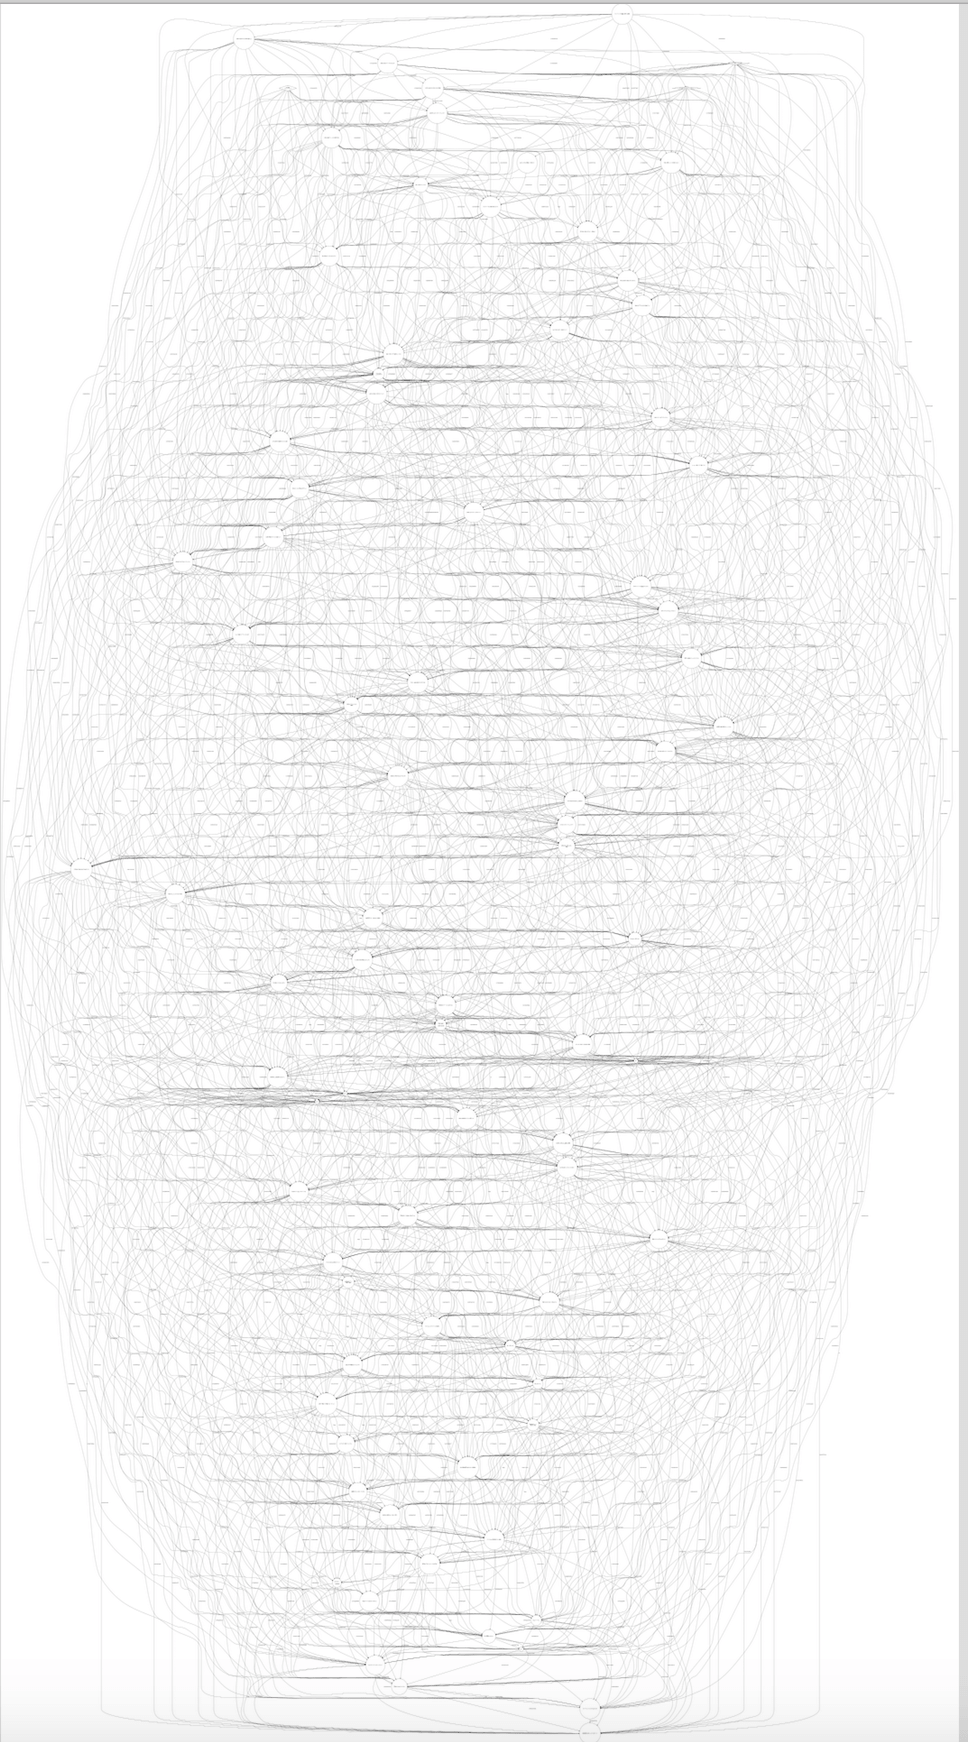
\includegraphics[width=\textwidth]{../images/5.Experiment/Graph=TF-IDF-min.png}
  \caption{比較手法2による繋がりグラフ}
  \label{Fig:GraphTF-IDF}
  \vspace{-10pt}
 \end{center}
\end{figure}
\end{comment}
%図\ref{Fig:GraphTF-IDF}で示されるように,発言の横の広がりが大きく,かなりの数の発言が話題を変えるものであると判定されていることが確認できる.
%以上の2つの比較手法の問題点に対する考察を踏まえて提案手法が比較手法と異なる点を考える.異なる点として,上位の単語のみを類似度計算に用いている点と分散表現を用いている点が挙げられる.
%比較手法2と違って,字面が異なっていても意味が類似していればが類似度が上がるようになり,結果として話題が変化したと判定する回減少し,比較手法2よりも高い適合率を示したと考えられる.
%図\ref{Fig:GraphFastText}に提案手法で発言の繋がりを図示したものを示す.
\begin{comment}
\begin{figure}[htbp]
 \begin{center}
  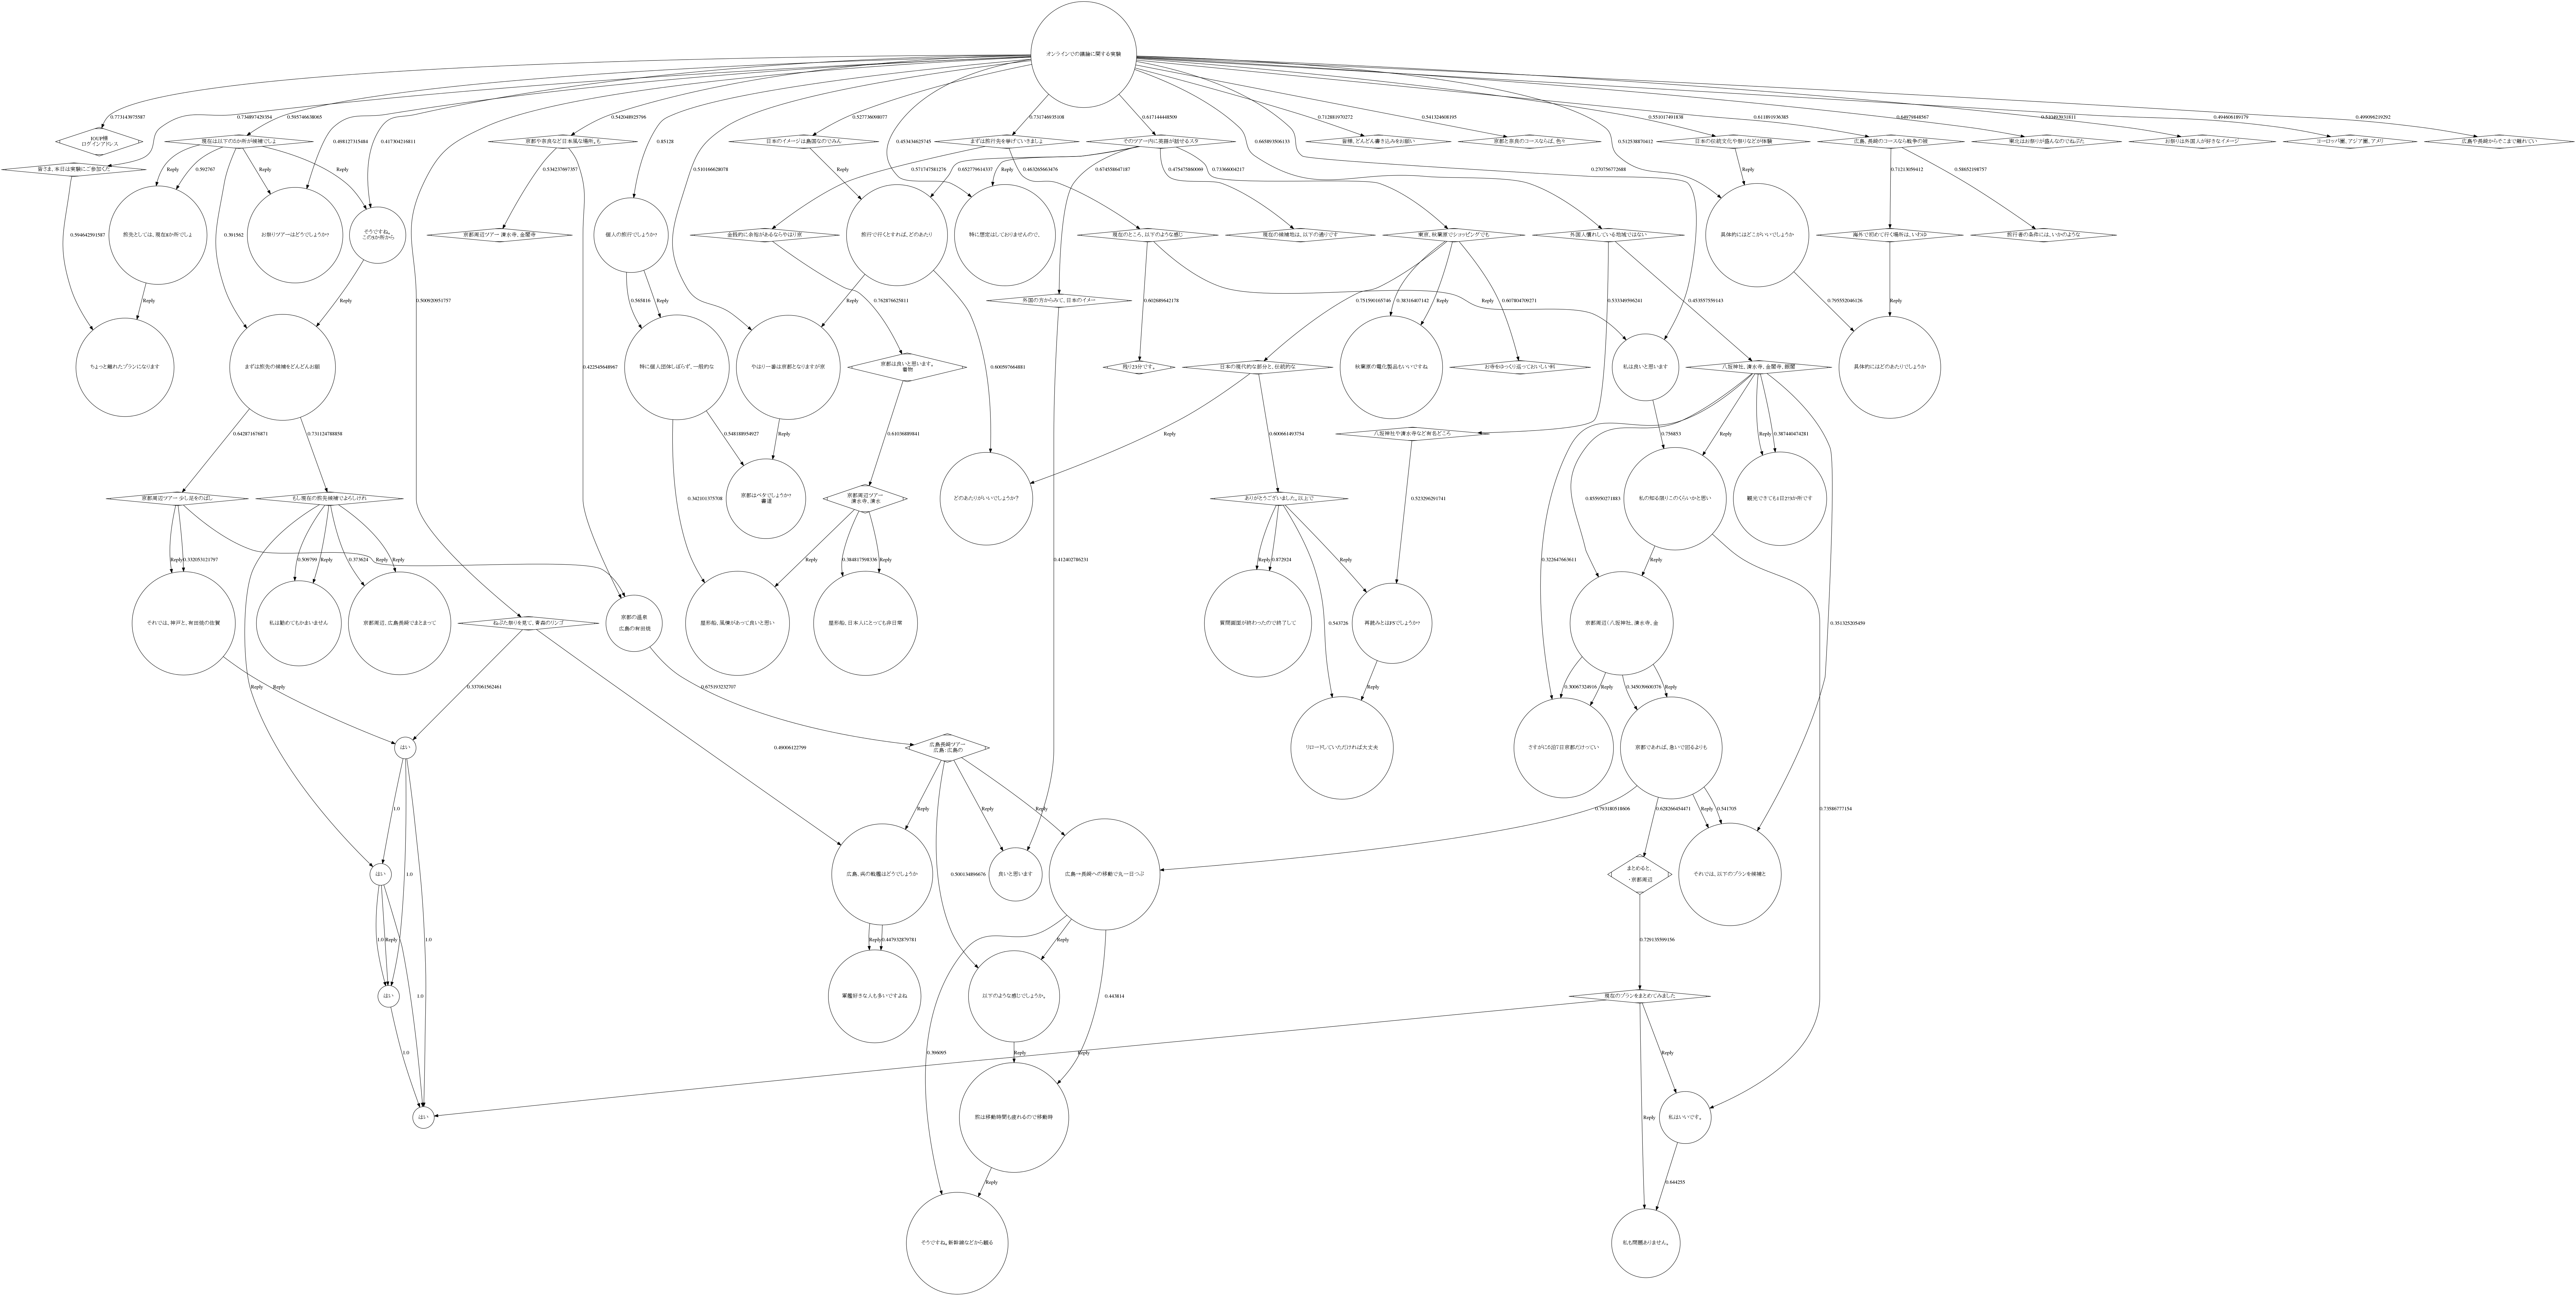
\includegraphics[width=\textwidth]{../images/5.Experiment/Graph=FastText-min.png}
  \caption{提案手法1による繋がりグラフ}
  \label{Fig:GraphFastText}
  \vspace{-10pt}
 \end{center}
\end{figure}
\end{comment}
%図\ref{Fig:GraphTF-IDF}とは違い,発言の横の広がりが小さめになっており,比較手法2に比べ類似度が高くなっていることが伺える.
%また,分散表現を用いることで字面の異なる単語でも類似性を示すことができるため,適合率と共に再現率を上昇させることに繋がったと考えられ,故に適合率と再現率の間に大きな差を生むこと無く判定をすることができたと考えられる.
%また,TF-DFを用いた手法が最も高いF値を示した理由として,TF-DFによる評価値の高い単語が議論の話題において重要な単語に該当していると考えられる.DFが高いことは頻繁に出現する単語であることを意味し,議論において重要な単語であると想定できる.事前にMeCabによってDF値の高いストップワードの除去を行っていたことも一因として考えられる.
%しかし,IDFを用いていない分,各発言の特徴的な単語が抽出されづらくなったことで抽出される単語がTF-IDFを用いる手法に比べて類似し,結果として類似度が高くなった可能性が高い.表\ref{table:result2}に示されているように話題を変えると判定された発言の割合が減少していることからも類似度が高くなったことが伺える.故に,他の提案手法に比べて,再現率の低下が大きくなったと考えられる.
\begin{comment}
\subsection*{考察\circled{3} 提案手法の精度は重み付けに依存する}
表\ref{table:FalseAlarmsRemark}, \ref{table:MissesRemark}にそれぞれ提案手法1で$FalseAlarms$,$Misses$となった発言の例を示す.
\begin{table}[htbp]
  \begin{tabular}{| c |  p{6cm} | p{5cm} |} \hline
     title & body  & 抽出単語 \\ \hline
     まずは旅先候補を&まずは旅先候補をどんどんお願いします。&どんどん,お願い,書き込み,皆様\\ \hline
     NULL &八坂神社、清水寺、金閣寺、銀閣寺、伏見稲荷大社、嵐山、有馬温泉 今あがっているのは、このぐらいでしょうか?&あがっ,今,伏見稲荷大社,嵐山,有馬温泉\\
     \hline
  \end{tabular}
  \caption{FalseAlarms発言データ} \label{table:FalseAlarmsRemark}
\end{table}
\begin{table}[htbp]
\begin{center}
  \begin{tabular}{| c | p{8cm} | p{6cm} |} \hline
     title & body & 抽出単語 \\ \hline
     NULL&やはり東京は人気ですよね、アキバ行きたいって外国のかたが多いイメージです & 外国,行き,多い,イメージ,アキバ \\ \hline
     NULL &  \shortstack{1日目大阪(USJ)\\
 2日目京都 (大原,嵐山,金閣寺,二年坂)\\
 3日目京都 (大原,嵐山,金閣寺,二年坂)\\
 4日目金沢\\
 5日目金沢\\
 6日目箱根\\
 7日目東京\\
 と言う感じでしょうか} & 金沢,金閣寺,二年坂,大原,嵐山\\
     \hline
  \end{tabular}
  \caption{Misses発言データ} \label{table:MissesRemark}
  \end{center}
\end{table}
まず,表\ref{table:FalseAlarmsRemark}の上段にあるような,議論の最初の方において意見を促すようなファシリテーターが行うような発言がfalseAlarmsとして誤判定されることが多かった.原因として過去に投稿された発言が少ないため他の発言との差が顕著になってしまったと考えられる.
\\
一方,表\ref{table:MissesRemark}の上段にあるような他の発言に対する雑談っぽさのある他の視点を提供しようとするような返信発言がmissesとして誤判定されることが多かった.原因として本研究における手法では返信関係にある2発言間の類似度は返信関係にない2発言間に比べて上がりやすくなっていることが考えられる.
\\
また,まとめを行う発言に弱いことが示された.原因としてまずはそもそも,表\ref{table:FalseAlarmsRemark},\ref{table:MissesRemark}の両方にまとめを行う発言があるように人間でも時と場合によって判断が分かれることが挙げられる.既に投稿されたまとめ発言との差やタイミング等,提案手法で考慮しきれていない要素が人の判断に影響していると考える.
他の原因として,含まれている単語数が多いことが挙げられる.以前の発言に含まれている単語が集まっていることから,表\ref{table:FalseAlarmsRemark}の下段で示されているように偏り無く抽出されることや,逆に表\ref{table:MissesRemark}の下段で示されている発言のように偏った内容の抽出がされることがある.上記のような不確定要素が結果に影響を与えたと考える.
\end{comment}
%\subsection*{考察\circled{3} 同じスレッドに属する2発言を同じ話題だと規定することで性能がある程度まで上昇する}
\subsection*{考察\circled{3} 2発言が同じスレッドである場合の補正値を高くすることで性能がある程度まで上昇する}
$\alpha$=0.85が最も良い$\alpha$の数値であったが,最良であった要因として最も大きいのは類似度閾値の値よりも大きかったことであると考える.
すなわち,2つの発言が返信関係によって同じスレッドに属している場合,同じ話題であると規定することによって現在の提案手法では性能がある程度まで上昇することが分かった.

しかし,話題変化を起こすとタグ付けで判定された発言の内,他の発言と同じスレッドに属しているものは$55$\%である.
すなわち,話題を変える発言の半数以上は返信発言であり,$\alpha$=0.85の条件下では見逃されていることが分かる.

故に,2つの発言が返信関係によって同じスレッドに属している場合,同じ話題であると判定することは必ずしも性能が上昇するわけではなく,あくまで「ある程度まで」であることも分かった.
%\subsection*{考察\circled{4} LexRankで用いる文章数は50で十分である}
%提案手法1と提案手法4の間に精度の大きな差はなく,LexRankの文章数を表すパラメーターnは50で十分であることが示された.

\section{結言}
\label{exp:conclusion}
本章では本研究で提案する話題変化の判定手法が有用であることを実験により確認した.伊藤孝行研究室の学生に,COLLAGREEで行われた議論データに対して基準を満たすと思われる発言にタグを付けてもらって評価データとした.評価実験では発言の内容に関係なく常に通知する手法と分散表現の代わりにTF-IDFを用いて発言をベクトル化する手法及びLDAを用いて発言をベクトル化する手法と比較した.

%実験の結果,提案手法は比較手法よりも性能が上であること,提案手法での単語抽出が性能上昇に貢献していること,新しいスレッドを立てる発言は話題変化を起こしやすい傾向にあることがわかった.
実験の結果,以下のことがわかった.
\begin{itemize}
  \item 提案手法は再現率と適合率の間の差が最も小さく,比較手法よりも良い性能を示す
  \item 単語抽出を行うことで発言の平均ベクトル間の差が出やすくなり,性能が上昇する
  \item 同じスレッドに属する2発言を同じ話題だと規定することで性能が上昇するが,限界がある
\end{itemize}

 %-------------------------------------------------------------------------------
 \expandafter\ifx\csname MasterFile\endcsname\relax
	\def\BibFile{hoge}
	\expandafter\ifx\csname MasterFile\endcsname\relax
\def\SubFile{hoge}
\documentclass[a4j,12pt,twoside,openany]{jreport}
%\nofiles %tocファイルを更新させない
%\documentclass[12pt,a4j,twoside,openany]{jsbook}
\usepackage[dvipdfmx]{graphicx}
\usepackage{../dspc} % ベースラインスキップの指定
\usepackage{../slashbox} % 表に斜線を入れる
%\usepackage{../mediabb}
\usepackage{fancyvrb} % Verbatim環境
\usepackage{fancyhdr} % Headerの下線付き章見出し
\usepackage{here} % float[H]
\usepackage{multirow}
\usepackage{hhline} % 表の罫線の角を美しくする
\usepackage{amsmath} %コレがないとcasesが動かない
\usepackage{amsfonts} % 数学用フォント
\usepackage{bm} % 数式環境での bold
\usepackage{algorithm}
\usepackage{algorithmicx}
\usepackage[noend]{algpseudocode}%\procedureはここに含まれる
\usepackage[flushleft]{threeparttable} % 脚注付きテーブル
\usepackage{enumitem}
\usepackage{comment}
\usepackage{fancybox}
%\usepackage{csvsimple,booktabs,siunitx}
%\usepackage{filecontents}
\usepackage{ulinej}


\setlength{\evensidemargin}{5pt}
\setlength{\oddsidemargin}{40pt}
%\setlength{\headheight}{16.5pt}
%%\setlength{\headheight}{30pt}
\setcounter{secnumdepth}{3}
\setlist[description]{leftmargin=2\parindent,labelindent=\parindent}

\makeatletter
\def\@makechapterhead#1{%
	\vspace*{50\p@}%
	{
		\parindent \z@ \raggedright \normalfont
		\ifnum \c@secnumdepth >\m@ne
		% \if@mainmatter
			\huge\bfseries\@chapapp\thechapter\@chappos
			\par\nobreak
			\vskip 20\p@
		% \fi
		\fi
		\interlinepenalty\@M
		\Huge\bfseries #1\par\nobreak
		\vskip 40\p@
	}
}

%新しいコマンド定義
\newcounter{linenumber}
\newenvironment{listing}{%
  \begin{list}{%
    \small\arabic{linenumber}:}{%
      \usecounter{linenumber}%
      \setlength{\baselineskip}{18pt}%
      \setlength{\itemsep}{0pt}%
      \setlength{\parsep}{0pt}}}%
 {\end{list}}
\newcommand{\figcaption}[1]{\def\@captype{figure}\caption{#1}}
\newcommand{\tblcaption}[1]{\def\@captype{table}\caption{#1}}
\newcommand{\norm}[1]{\left\| #1 \right\|}
\newcommand{\cc}[1]{\multicolumn{1}{|c|}{#1}}
\newcommand{\circled}[1]{\raisebox{.5pt}{\textcircled{\raisebox{-.9pt} {#1}}}}
\newcommand{\specialcell}[2][c]{%
  \begin{tabular}[#1]{@{}c@{}}#2\end{tabular}}
\makeatother
%===============================================================================
\expandafter\ifx\csname SubFile\endcsname\relax
\begin{document}
\def\MasterFile{hoge}
%-------------------------------------------------------------------------------
%\maketitle
\thispagestyle{empty}
\documentclass[a4j,12pt]{jarticle}
% 外表紙

% 題名
\def\title{降水量予測のための\\Sequence-to-Sequenceモデルに基づく\\マルチモーダル学習}
% 著者
\def\author{林 政行}
% 入学年度(平成)
\def\year{24}
% 学籍番号
\def\number{24115113}
% 指導教官
\def\kyoukan{伊藤孝行}
% 指導教官役職
\def\kyoukanrank{教授}
% 提出日
\def\teisyutubi{平成28年2月8日}

\begin{document}
\pagestyle{empty}
\baselineskip=18pt

\begin{center}

\vspace*{2cm}

{\huge \textbf{卒業論文}}

\vspace*{3cm}

%\vrule width 10cm height 1pt depth 0pt



%(題目)
%\vspace{5pt}
%\hrule height 3pt
%\vspace{1zh}

\vrule width 6.25cm height 6pt depth -2pt
\makebox[1.5cm]{(題目)}
\vrule width 6.25cm height 6pt depth -2pt

{\LARGE {\title}}

\vspace{1zh}
%{\large {\subtitle}}
%\hrule height 3pt
\vrule width 14cm height 4pt depth 0pt

\vspace*{1cm}

指導教員 {\large {\kyoukan}} {\kyoukanrank}

%\vspace*{5cm}
\vfill

{\large 名古屋工業大学 情報工学科}

{\large 平成{\year}年度 入学 ({\number})}

\vspace*{1cm}

%{\huge\mc {\author}}

\underline{(氏名)\hspace{3zw}{\huge\mc {\author}}\hspace{3zw}}

\vspace*{1cm}

({\teisyutubi}提出)

\vspace{2cm}
\end{center}

\end{document}
\begin{titlepage}

% 題名
\def\title{分散表現を用いた\\話題変化判定}
% 補助題名
\def\subtitle{卒業論文}
% 著者
\def\author{芳野 魁}
% 入学年度(平成)
\def\year{29}
% 学籍番号
\def\number{26115162}
% 指導教官
\def\kyoukan{伊藤 孝行}
% 指導教官役職
\def\kyoukanrank{教授}
% 提出日
\def\teisyutubi{平成29年9月19日}

\pagestyle{empty}

\begin{center}

\vspace*{20mm}
{\Large\mc 平成29年度 \hspace{7mm} 卒 業 論 文}
\vspace{15mm}

%\setlength{\unitlength}{1mm}
\begin{picture}(100,60)
  \put(0,0){\makebox(100,60){\huge\bf\shortstack{\title}}}
\end{picture}
\\
%\begin{picture}(100,5)
%  \put(0,0){\makebox(100,5){\Large\bf\shortstack{\subtitle}}}
%\end{picture}
\end{center}
\vspace{10mm}
\begin{flushright}
\begin{tabular}{ll}
{\large 提出日} & {\large {\teisyutubi}} \\
{\large 所属}  & {\large 名古屋工業大学 情報工学科} \\
{\large 指導教員} & {\large {\kyoukan} {\kyoukanrank}} \\
 & \\
{\large 入学年度} & {\large 平成{\year}年度入学}\\
{\large 学籍番号} &{\large {\number}} \\
 & \\
%{\large 氏名} & {\huge {\author}}
{\large 氏名} & {\huge\mc {\author}}
\end{tabular}
\end{flushright}

\end{titlepage}

%\addcontentsline{toc}{chapter}{表紙}
\thispagestyle{empty}
\mbox{}\newpage
%===============================================================================
%\frontmatter
%===============================================================================
%\mainmatter
%-------------------------------------------------------------------------------
\pagenumbering{arabic}
\cleardoublepage
\expandafter\ifx\csname MasterFile\endcsname\relax
\def\SubFile{hoge}
\input{../thesis/thesis}
\begin{document}
\fi
%-------------------------------------------------------------------------------
\cleardoublepage
\chapter*{論文要旨}\addcontentsline{toc}{chapter}{論文要旨}
近年,Web上での大規模な議論活動が活発になっているが,現在一般的に使われている "2ちゃんねる" や "Twitter" といったシステムでは整理や収束を行うことが困難である.困難である原因として,議論の管理を行う者がいないことが挙げられる.
議論を収束させるには議論のマネジメントを行う人物が必要である.
%
大規模意見集約システムCOLLAGREEではファシリテーターと呼ばれる人物が議論のマネジメントを行っている.
しかし,ファシリテーターは人間であり,長時間に渡って大人数での議論の動向をマネジメントし続けるのは困難である.
%
COLLAGREEで大規模な議論を収束させるためには,ファシリテーターが必要な時にだけ画面を見るようにして画面に向き合う時間を減らす工夫があることが望ましい.ファシリテーターが画面を見るべきタイミングは議論の話題が変化したときである.以前の議論の内容から外れた発言がされた時,ファシリテーターが適切に発言することで,脱線や炎上を避けて議論を収束させることができる.
すなわち,ファシリテーターの代わりに自動的に議論中の話題の変化を事前に判定することが求められている.
%
現在,COLLAGREE上で使用されている議論支援システムは投稿支援システムと議論可視化システムの2つに大別できる.
投稿支援システムはポイント機能やファシリテーションフレーズ簡易投稿機能のように,ユーザーが投稿をする際に何らかの補助やリアクションを行う.現行の機能では選択肢の提示に留まっており,作業量を減らすことには繋がりにくい。
一方,議論可視化システムは議論ツリーやキーワード抽出のように,ユーザーにスレッドとは異なる議論の見方を提供する.現行の機能では議論を見やすくすることに重点が置かれており,議論の把握の助けにはなるが画面に向き合う時間を減らすことにはなりにくい.むしろ,作業量を増やすことになり得る機能もある.
\begin{comment}
ポイント機能(ユーザの議論行動を活性化)-1
ファシリテーションフレーズ簡易投稿機能-1
議論ツリー-2
1文の要約,スレッドの要約,クラスタリング,返信意見の極性判定-2
ファシリテーションスタンプ-1
キーワード抽出-2
いいね機能-1
いいねランキング-2
投票機能-1
議論フェーズ機能-2
1-意見を出す、投稿をする際に補助や選択肢、リアクションを与える
2-議論の別の見方を提供する
\end{comment}
%
近年,自然言語処理の分野において分散表現が多くの研究で使われており,機械翻訳を始めとする単語の意味が重要となる分野で精度の向上が確認されている.分散表現を用いることで,人間に近い精度で話題の変化を観測することが可能となる.
%
以上のような背景を踏まえて,分散表現を用いて,話題の変化を観測し,話題の変化が確認された時にファシリテーターに伝えることが望ましい.
話題の変化の観測は,発言中に現れる単語の関連度合いの計算と見なすことができる.
分散表現を用いることで単語間の類似度を求めることができる,値が大きいほど単語がそれぞれ類似した実数ベクトルであることを表す.単語Aと単語Bの実数ベクトルが類似しているとは,単語Aと共に使われることの多い単語と単語Bと共に使われることの多い単語が多く共通していることを示す.故に,分散表現を使って単語の関連度を計算することができる.
%
発言文から単語を選ぶ際には自動要約を用いる.発言文から重要でない単語を取り除くことで関連度の計算の精度を高めることが可能となる.
%
本論文では,分散表現を用いて議論中での発言に含まれる単語の関連度を計算し,話題の変化を観測する手法を提案する.
%
提案手法は,既存の抽出的要約手法を用いて選ばれた単語の関連度を計算する手法,Seq2Seqによる生成的要約を用いて生成された単語の関連度を計算する手法,オントロジーを用いて求められた単語の関連度を計算する手法の3つである.
提案した3つの手法により,議論中の話題の変化の観測の評価実験を行い,各手法の評価を行う.
評価実験によって,提案手法を用いることで人間の代わりに自動的に話題の変化を観測できることを確認する.
%
 \begin{comment}
大規模な議論では意見を共有することは可能であるが,議論を整理させることや収束させることは難しい.以上から大規模意見集約システムCOLLAGREEが開発された.本システムではWeb上で適切に大規模な議論を行うことができるように議論をマネジメントするファシリテーターを導入した.
過去の実験ではファシリテーターの存在が議論の集約に大きな役割を果たしていることが認識されており,大規模な議論のためにファシリテータは必要である.しかし,議論の規模に伴って議論時間が長くなる傾向があり,同時にファシリテーターは常に議論の動向を見続ける必要がある.故に,議論の規模が大きくなればなるほどファシリテーターは長時間かつ大規模な議論の動向の監視によって大きな負担がかかる.大規模な議論が増加する傾向を踏まえるとファシリテーターにかかる負担を軽減する支援が必要となることは明白である.
また,近年自然言語処理の分野において分散表現が多くの研究で使われており,機械翻訳を始めとする複数の分野で精度の向上が確認されている.まだ適応されていない分野でも結果の向上が期待できる.
従って,本研究では負担軽減の1つとして分散表現を用いて議論中での話題の変化を人間の代わりに検知することでファシリテーターの負担を軽減することを目指す.
-----------------

\end{comment}
%-------------------------------------------------------------------------------
\expandafter\ifx\csname MasterFile\endcsname\relax
\end{document}
\fi

%-------------------------------------------------------------------------------
\clearpage
\addcontentsline{toc}{chapter}{目次}
\tableofcontents

\clearpage
\addcontentsline{toc}{chapter}{図目次}
\listoffigures

\clearpage
\addcontentsline{toc}{chapter}{表目次}
\listoftables

%-------------------------------------------------------------------------------

%=====================
\pagestyle{fancy} % Headerをつける
\renewcommand{\sectionmark}[1]{\markright{\thesection\ \ \ #1}}
\renewcommand{\chaptermark}[1]{\markboth{#1}{}}
\lhead{}
\chead{}
\lfoot{}
\rfoot{}%-------------------------------------------------------------------------------
\expandafter\ifx\csname MasterFile\endcsname\relax
\def\SubFile{hoge}
\input{../thesis/thesis}
\begin{document}
\fi
%-------------------------------------------------------------------------------
\cleardoublepage
\chapter*{論文要旨}\addcontentsline{toc}{chapter}{論文要旨}
近年,Web上での大規模な議論活動が活発になっているが,現在一般的に使われている "2ちゃんねる" や "Twitter" といったシステムでは整理や収束を行うことが困難である.困難である原因として,議論の管理を行う者がいないことが挙げられる.
議論を収束させるには議論のマネジメントを行う人物が必要である.
%
大規模意見集約システムCOLLAGREEではファシリテーターと呼ばれる人物が議論のマネジメントを行っている.
しかし,ファシリテーターは人間であり,長時間に渡って大人数での議論の動向をマネジメントし続けるのは困難である.
%
COLLAGREEで大規模な議論を収束させるためには,ファシリテーターが必要な時にだけ画面を見るようにして画面に向き合う時間を減らす工夫があることが望ましい.ファシリテーターが画面を見るべきタイミングは議論の話題が変化したときである.以前の議論の内容から外れた発言がされた時,ファシリテーターが適切に発言することで,脱線や炎上を避けて議論を収束させることができる.
すなわち,ファシリテーターの代わりに自動的に議論中の話題の変化を事前に判定することが求められている.
%
現在,COLLAGREE上で使用されている議論支援システムは投稿支援システムと議論可視化システムの2つに大別できる.
投稿支援システムはポイント機能やファシリテーションフレーズ簡易投稿機能のように,ユーザーが投稿をする際に何らかの補助やリアクションを行う.現行の機能では選択肢の提示に留まっており,作業量を減らすことには繋がりにくい。
一方,議論可視化システムは議論ツリーやキーワード抽出のように,ユーザーにスレッドとは異なる議論の見方を提供する.現行の機能では議論を見やすくすることに重点が置かれており,議論の把握の助けにはなるが画面に向き合う時間を減らすことにはなりにくい.むしろ,作業量を増やすことになり得る機能もある.
\begin{comment}
ポイント機能(ユーザの議論行動を活性化)-1
ファシリテーションフレーズ簡易投稿機能-1
議論ツリー-2
1文の要約,スレッドの要約,クラスタリング,返信意見の極性判定-2
ファシリテーションスタンプ-1
キーワード抽出-2
いいね機能-1
いいねランキング-2
投票機能-1
議論フェーズ機能-2
1-意見を出す、投稿をする際に補助や選択肢、リアクションを与える
2-議論の別の見方を提供する
\end{comment}
%
近年,自然言語処理の分野において分散表現が多くの研究で使われており,機械翻訳を始めとする単語の意味が重要となる分野で精度の向上が確認されている.分散表現を用いることで,人間に近い精度で話題の変化を観測することが可能となる.
%
以上のような背景を踏まえて,分散表現を用いて,話題の変化を観測し,話題の変化が確認された時にファシリテーターに伝えることが望ましい.
話題の変化の観測は,発言中に現れる単語の関連度合いの計算と見なすことができる.
分散表現を用いることで単語間の類似度を求めることができる,値が大きいほど単語がそれぞれ類似した実数ベクトルであることを表す.単語Aと単語Bの実数ベクトルが類似しているとは,単語Aと共に使われることの多い単語と単語Bと共に使われることの多い単語が多く共通していることを示す.故に,分散表現を使って単語の関連度を計算することができる.
%
発言文から単語を選ぶ際には自動要約を用いる.発言文から重要でない単語を取り除くことで関連度の計算の精度を高めることが可能となる.
%
本論文では,分散表現を用いて議論中での発言に含まれる単語の関連度を計算し,話題の変化を観測する手法を提案する.
%
提案手法は,既存の抽出的要約手法を用いて選ばれた単語の関連度を計算する手法,Seq2Seqによる生成的要約を用いて生成された単語の関連度を計算する手法,オントロジーを用いて求められた単語の関連度を計算する手法の3つである.
提案した3つの手法により,議論中の話題の変化の観測の評価実験を行い,各手法の評価を行う.
評価実験によって,提案手法を用いることで人間の代わりに自動的に話題の変化を観測できることを確認する.
%
 \begin{comment}
大規模な議論では意見を共有することは可能であるが,議論を整理させることや収束させることは難しい.以上から大規模意見集約システムCOLLAGREEが開発された.本システムではWeb上で適切に大規模な議論を行うことができるように議論をマネジメントするファシリテーターを導入した.
過去の実験ではファシリテーターの存在が議論の集約に大きな役割を果たしていることが認識されており,大規模な議論のためにファシリテータは必要である.しかし,議論の規模に伴って議論時間が長くなる傾向があり,同時にファシリテーターは常に議論の動向を見続ける必要がある.故に,議論の規模が大きくなればなるほどファシリテーターは長時間かつ大規模な議論の動向の監視によって大きな負担がかかる.大規模な議論が増加する傾向を踏まえるとファシリテーターにかかる負担を軽減する支援が必要となることは明白である.
また,近年自然言語処理の分野において分散表現が多くの研究で使われており,機械翻訳を始めとする複数の分野で精度の向上が確認されている.まだ適応されていない分野でも結果の向上が期待できる.
従って,本研究では負担軽減の1つとして分散表現を用いて議論中での話題の変化を人間の代わりに検知することでファシリテーターの負担を軽減することを目指す.
-----------------

\end{comment}
%-------------------------------------------------------------------------------
\expandafter\ifx\csname MasterFile\endcsname\relax
\end{document}
\fi

%-------------------------------------------------------------------------------
\expandafter\ifx\csname MasterFile\endcsname\relax
\def\SubFile{hoge}
\input{../thesis/thesis}
\begin{document}
\fi
%-------------------------------------------------------------------------------
\cleardoublepage
\chapter*{論文要旨}\addcontentsline{toc}{chapter}{論文要旨}
近年,Web上での大規模な議論活動が活発になっているが,現在一般的に使われている "2ちゃんねる" や "Twitter" といったシステムでは整理や収束を行うことが困難である.困難である原因として,議論の管理を行う者がいないことが挙げられる.
議論を収束させるには議論のマネジメントを行う人物が必要である.
%
大規模意見集約システムCOLLAGREEではファシリテーターと呼ばれる人物が議論のマネジメントを行っている.
しかし,ファシリテーターは人間であり,長時間に渡って大人数での議論の動向をマネジメントし続けるのは困難である.
%
COLLAGREEで大規模な議論を収束させるためには,ファシリテーターが必要な時にだけ画面を見るようにして画面に向き合う時間を減らす工夫があることが望ましい.ファシリテーターが画面を見るべきタイミングは議論の話題が変化したときである.以前の議論の内容から外れた発言がされた時,ファシリテーターが適切に発言することで,脱線や炎上を避けて議論を収束させることができる.
すなわち,ファシリテーターの代わりに自動的に議論中の話題の変化を事前に判定することが求められている.
%
現在,COLLAGREE上で使用されている議論支援システムは投稿支援システムと議論可視化システムの2つに大別できる.
投稿支援システムはポイント機能やファシリテーションフレーズ簡易投稿機能のように,ユーザーが投稿をする際に何らかの補助やリアクションを行う.現行の機能では選択肢の提示に留まっており,作業量を減らすことには繋がりにくい。
一方,議論可視化システムは議論ツリーやキーワード抽出のように,ユーザーにスレッドとは異なる議論の見方を提供する.現行の機能では議論を見やすくすることに重点が置かれており,議論の把握の助けにはなるが画面に向き合う時間を減らすことにはなりにくい.むしろ,作業量を増やすことになり得る機能もある.
\begin{comment}
ポイント機能(ユーザの議論行動を活性化)-1
ファシリテーションフレーズ簡易投稿機能-1
議論ツリー-2
1文の要約,スレッドの要約,クラスタリング,返信意見の極性判定-2
ファシリテーションスタンプ-1
キーワード抽出-2
いいね機能-1
いいねランキング-2
投票機能-1
議論フェーズ機能-2
1-意見を出す、投稿をする際に補助や選択肢、リアクションを与える
2-議論の別の見方を提供する
\end{comment}
%
近年,自然言語処理の分野において分散表現が多くの研究で使われており,機械翻訳を始めとする単語の意味が重要となる分野で精度の向上が確認されている.分散表現を用いることで,人間に近い精度で話題の変化を観測することが可能となる.
%
以上のような背景を踏まえて,分散表現を用いて,話題の変化を観測し,話題の変化が確認された時にファシリテーターに伝えることが望ましい.
話題の変化の観測は,発言中に現れる単語の関連度合いの計算と見なすことができる.
分散表現を用いることで単語間の類似度を求めることができる,値が大きいほど単語がそれぞれ類似した実数ベクトルであることを表す.単語Aと単語Bの実数ベクトルが類似しているとは,単語Aと共に使われることの多い単語と単語Bと共に使われることの多い単語が多く共通していることを示す.故に,分散表現を使って単語の関連度を計算することができる.
%
発言文から単語を選ぶ際には自動要約を用いる.発言文から重要でない単語を取り除くことで関連度の計算の精度を高めることが可能となる.
%
本論文では,分散表現を用いて議論中での発言に含まれる単語の関連度を計算し,話題の変化を観測する手法を提案する.
%
提案手法は,既存の抽出的要約手法を用いて選ばれた単語の関連度を計算する手法,Seq2Seqによる生成的要約を用いて生成された単語の関連度を計算する手法,オントロジーを用いて求められた単語の関連度を計算する手法の3つである.
提案した3つの手法により,議論中の話題の変化の観測の評価実験を行い,各手法の評価を行う.
評価実験によって,提案手法を用いることで人間の代わりに自動的に話題の変化を観測できることを確認する.
%
 \begin{comment}
大規模な議論では意見を共有することは可能であるが,議論を整理させることや収束させることは難しい.以上から大規模意見集約システムCOLLAGREEが開発された.本システムではWeb上で適切に大規模な議論を行うことができるように議論をマネジメントするファシリテーターを導入した.
過去の実験ではファシリテーターの存在が議論の集約に大きな役割を果たしていることが認識されており,大規模な議論のためにファシリテータは必要である.しかし,議論の規模に伴って議論時間が長くなる傾向があり,同時にファシリテーターは常に議論の動向を見続ける必要がある.故に,議論の規模が大きくなればなるほどファシリテーターは長時間かつ大規模な議論の動向の監視によって大きな負担がかかる.大規模な議論が増加する傾向を踏まえるとファシリテーターにかかる負担を軽減する支援が必要となることは明白である.
また,近年自然言語処理の分野において分散表現が多くの研究で使われており,機械翻訳を始めとする複数の分野で精度の向上が確認されている.まだ適応されていない分野でも結果の向上が期待できる.
従って,本研究では負担軽減の1つとして分散表現を用いて議論中での話題の変化を人間の代わりに検知することでファシリテーターの負担を軽減することを目指す.
-----------------

\end{comment}
%-------------------------------------------------------------------------------
\expandafter\ifx\csname MasterFile\endcsname\relax
\end{document}
\fi

%-------------------------------------------------------------------------------
\expandafter\ifx\csname MasterFile\endcsname\relax
\def\SubFile{hoge}
\input{../thesis/thesis}
\begin{document}
\fi
%-------------------------------------------------------------------------------
\cleardoublepage
\chapter*{論文要旨}\addcontentsline{toc}{chapter}{論文要旨}
近年,Web上での大規模な議論活動が活発になっているが,現在一般的に使われている "2ちゃんねる" や "Twitter" といったシステムでは整理や収束を行うことが困難である.困難である原因として,議論の管理を行う者がいないことが挙げられる.
議論を収束させるには議論のマネジメントを行う人物が必要である.
%
大規模意見集約システムCOLLAGREEではファシリテーターと呼ばれる人物が議論のマネジメントを行っている.
しかし,ファシリテーターは人間であり,長時間に渡って大人数での議論の動向をマネジメントし続けるのは困難である.
%
COLLAGREEで大規模な議論を収束させるためには,ファシリテーターが必要な時にだけ画面を見るようにして画面に向き合う時間を減らす工夫があることが望ましい.ファシリテーターが画面を見るべきタイミングは議論の話題が変化したときである.以前の議論の内容から外れた発言がされた時,ファシリテーターが適切に発言することで,脱線や炎上を避けて議論を収束させることができる.
すなわち,ファシリテーターの代わりに自動的に議論中の話題の変化を事前に判定することが求められている.
%
現在,COLLAGREE上で使用されている議論支援システムは投稿支援システムと議論可視化システムの2つに大別できる.
投稿支援システムはポイント機能やファシリテーションフレーズ簡易投稿機能のように,ユーザーが投稿をする際に何らかの補助やリアクションを行う.現行の機能では選択肢の提示に留まっており,作業量を減らすことには繋がりにくい。
一方,議論可視化システムは議論ツリーやキーワード抽出のように,ユーザーにスレッドとは異なる議論の見方を提供する.現行の機能では議論を見やすくすることに重点が置かれており,議論の把握の助けにはなるが画面に向き合う時間を減らすことにはなりにくい.むしろ,作業量を増やすことになり得る機能もある.
\begin{comment}
ポイント機能(ユーザの議論行動を活性化)-1
ファシリテーションフレーズ簡易投稿機能-1
議論ツリー-2
1文の要約,スレッドの要約,クラスタリング,返信意見の極性判定-2
ファシリテーションスタンプ-1
キーワード抽出-2
いいね機能-1
いいねランキング-2
投票機能-1
議論フェーズ機能-2
1-意見を出す、投稿をする際に補助や選択肢、リアクションを与える
2-議論の別の見方を提供する
\end{comment}
%
近年,自然言語処理の分野において分散表現が多くの研究で使われており,機械翻訳を始めとする単語の意味が重要となる分野で精度の向上が確認されている.分散表現を用いることで,人間に近い精度で話題の変化を観測することが可能となる.
%
以上のような背景を踏まえて,分散表現を用いて,話題の変化を観測し,話題の変化が確認された時にファシリテーターに伝えることが望ましい.
話題の変化の観測は,発言中に現れる単語の関連度合いの計算と見なすことができる.
分散表現を用いることで単語間の類似度を求めることができる,値が大きいほど単語がそれぞれ類似した実数ベクトルであることを表す.単語Aと単語Bの実数ベクトルが類似しているとは,単語Aと共に使われることの多い単語と単語Bと共に使われることの多い単語が多く共通していることを示す.故に,分散表現を使って単語の関連度を計算することができる.
%
発言文から単語を選ぶ際には自動要約を用いる.発言文から重要でない単語を取り除くことで関連度の計算の精度を高めることが可能となる.
%
本論文では,分散表現を用いて議論中での発言に含まれる単語の関連度を計算し,話題の変化を観測する手法を提案する.
%
提案手法は,既存の抽出的要約手法を用いて選ばれた単語の関連度を計算する手法,Seq2Seqによる生成的要約を用いて生成された単語の関連度を計算する手法,オントロジーを用いて求められた単語の関連度を計算する手法の3つである.
提案した3つの手法により,議論中の話題の変化の観測の評価実験を行い,各手法の評価を行う.
評価実験によって,提案手法を用いることで人間の代わりに自動的に話題の変化を観測できることを確認する.
%
 \begin{comment}
大規模な議論では意見を共有することは可能であるが,議論を整理させることや収束させることは難しい.以上から大規模意見集約システムCOLLAGREEが開発された.本システムではWeb上で適切に大規模な議論を行うことができるように議論をマネジメントするファシリテーターを導入した.
過去の実験ではファシリテーターの存在が議論の集約に大きな役割を果たしていることが認識されており,大規模な議論のためにファシリテータは必要である.しかし,議論の規模に伴って議論時間が長くなる傾向があり,同時にファシリテーターは常に議論の動向を見続ける必要がある.故に,議論の規模が大きくなればなるほどファシリテーターは長時間かつ大規模な議論の動向の監視によって大きな負担がかかる.大規模な議論が増加する傾向を踏まえるとファシリテーターにかかる負担を軽減する支援が必要となることは明白である.
また,近年自然言語処理の分野において分散表現が多くの研究で使われており,機械翻訳を始めとする複数の分野で精度の向上が確認されている.まだ適応されていない分野でも結果の向上が期待できる.
従って,本研究では負担軽減の1つとして分散表現を用いて議論中での話題の変化を人間の代わりに検知することでファシリテーターの負担を軽減することを目指す.
-----------------

\end{comment}
%-------------------------------------------------------------------------------
\expandafter\ifx\csname MasterFile\endcsname\relax
\end{document}
\fi

%-------------------------------------------------------------------------------
\expandafter\ifx\csname MasterFile\endcsname\relax
\def\SubFile{hoge}
\input{../thesis/thesis}
\begin{document}
\fi
%-------------------------------------------------------------------------------
\cleardoublepage
\chapter*{論文要旨}\addcontentsline{toc}{chapter}{論文要旨}
近年,Web上での大規模な議論活動が活発になっているが,現在一般的に使われている "2ちゃんねる" や "Twitter" といったシステムでは整理や収束を行うことが困難である.困難である原因として,議論の管理を行う者がいないことが挙げられる.
議論を収束させるには議論のマネジメントを行う人物が必要である.
%
大規模意見集約システムCOLLAGREEではファシリテーターと呼ばれる人物が議論のマネジメントを行っている.
しかし,ファシリテーターは人間であり,長時間に渡って大人数での議論の動向をマネジメントし続けるのは困難である.
%
COLLAGREEで大規模な議論を収束させるためには,ファシリテーターが必要な時にだけ画面を見るようにして画面に向き合う時間を減らす工夫があることが望ましい.ファシリテーターが画面を見るべきタイミングは議論の話題が変化したときである.以前の議論の内容から外れた発言がされた時,ファシリテーターが適切に発言することで,脱線や炎上を避けて議論を収束させることができる.
すなわち,ファシリテーターの代わりに自動的に議論中の話題の変化を事前に判定することが求められている.
%
現在,COLLAGREE上で使用されている議論支援システムは投稿支援システムと議論可視化システムの2つに大別できる.
投稿支援システムはポイント機能やファシリテーションフレーズ簡易投稿機能のように,ユーザーが投稿をする際に何らかの補助やリアクションを行う.現行の機能では選択肢の提示に留まっており,作業量を減らすことには繋がりにくい。
一方,議論可視化システムは議論ツリーやキーワード抽出のように,ユーザーにスレッドとは異なる議論の見方を提供する.現行の機能では議論を見やすくすることに重点が置かれており,議論の把握の助けにはなるが画面に向き合う時間を減らすことにはなりにくい.むしろ,作業量を増やすことになり得る機能もある.
\begin{comment}
ポイント機能(ユーザの議論行動を活性化)-1
ファシリテーションフレーズ簡易投稿機能-1
議論ツリー-2
1文の要約,スレッドの要約,クラスタリング,返信意見の極性判定-2
ファシリテーションスタンプ-1
キーワード抽出-2
いいね機能-1
いいねランキング-2
投票機能-1
議論フェーズ機能-2
1-意見を出す、投稿をする際に補助や選択肢、リアクションを与える
2-議論の別の見方を提供する
\end{comment}
%
近年,自然言語処理の分野において分散表現が多くの研究で使われており,機械翻訳を始めとする単語の意味が重要となる分野で精度の向上が確認されている.分散表現を用いることで,人間に近い精度で話題の変化を観測することが可能となる.
%
以上のような背景を踏まえて,分散表現を用いて,話題の変化を観測し,話題の変化が確認された時にファシリテーターに伝えることが望ましい.
話題の変化の観測は,発言中に現れる単語の関連度合いの計算と見なすことができる.
分散表現を用いることで単語間の類似度を求めることができる,値が大きいほど単語がそれぞれ類似した実数ベクトルであることを表す.単語Aと単語Bの実数ベクトルが類似しているとは,単語Aと共に使われることの多い単語と単語Bと共に使われることの多い単語が多く共通していることを示す.故に,分散表現を使って単語の関連度を計算することができる.
%
発言文から単語を選ぶ際には自動要約を用いる.発言文から重要でない単語を取り除くことで関連度の計算の精度を高めることが可能となる.
%
本論文では,分散表現を用いて議論中での発言に含まれる単語の関連度を計算し,話題の変化を観測する手法を提案する.
%
提案手法は,既存の抽出的要約手法を用いて選ばれた単語の関連度を計算する手法,Seq2Seqによる生成的要約を用いて生成された単語の関連度を計算する手法,オントロジーを用いて求められた単語の関連度を計算する手法の3つである.
提案した3つの手法により,議論中の話題の変化の観測の評価実験を行い,各手法の評価を行う.
評価実験によって,提案手法を用いることで人間の代わりに自動的に話題の変化を観測できることを確認する.
%
 \begin{comment}
大規模な議論では意見を共有することは可能であるが,議論を整理させることや収束させることは難しい.以上から大規模意見集約システムCOLLAGREEが開発された.本システムではWeb上で適切に大規模な議論を行うことができるように議論をマネジメントするファシリテーターを導入した.
過去の実験ではファシリテーターの存在が議論の集約に大きな役割を果たしていることが認識されており,大規模な議論のためにファシリテータは必要である.しかし,議論の規模に伴って議論時間が長くなる傾向があり,同時にファシリテーターは常に議論の動向を見続ける必要がある.故に,議論の規模が大きくなればなるほどファシリテーターは長時間かつ大規模な議論の動向の監視によって大きな負担がかかる.大規模な議論が増加する傾向を踏まえるとファシリテーターにかかる負担を軽減する支援が必要となることは明白である.
また,近年自然言語処理の分野において分散表現が多くの研究で使われており,機械翻訳を始めとする複数の分野で精度の向上が確認されている.まだ適応されていない分野でも結果の向上が期待できる.
従って,本研究では負担軽減の1つとして分散表現を用いて議論中での話題の変化を人間の代わりに検知することでファシリテーターの負担を軽減することを目指す.
-----------------

\end{comment}
%-------------------------------------------------------------------------------
\expandafter\ifx\csname MasterFile\endcsname\relax
\end{document}
\fi

%-------------------------------------------------------------------------------
\expandafter\ifx\csname MasterFile\endcsname\relax
\def\SubFile{hoge}
\input{../thesis/thesis}
\begin{document}
\fi
%-------------------------------------------------------------------------------
\cleardoublepage
\chapter*{論文要旨}\addcontentsline{toc}{chapter}{論文要旨}
近年,Web上での大規模な議論活動が活発になっているが,現在一般的に使われている "2ちゃんねる" や "Twitter" といったシステムでは整理や収束を行うことが困難である.困難である原因として,議論の管理を行う者がいないことが挙げられる.
議論を収束させるには議論のマネジメントを行う人物が必要である.
%
大規模意見集約システムCOLLAGREEではファシリテーターと呼ばれる人物が議論のマネジメントを行っている.
しかし,ファシリテーターは人間であり,長時間に渡って大人数での議論の動向をマネジメントし続けるのは困難である.
%
COLLAGREEで大規模な議論を収束させるためには,ファシリテーターが必要な時にだけ画面を見るようにして画面に向き合う時間を減らす工夫があることが望ましい.ファシリテーターが画面を見るべきタイミングは議論の話題が変化したときである.以前の議論の内容から外れた発言がされた時,ファシリテーターが適切に発言することで,脱線や炎上を避けて議論を収束させることができる.
すなわち,ファシリテーターの代わりに自動的に議論中の話題の変化を事前に判定することが求められている.
%
現在,COLLAGREE上で使用されている議論支援システムは投稿支援システムと議論可視化システムの2つに大別できる.
投稿支援システムはポイント機能やファシリテーションフレーズ簡易投稿機能のように,ユーザーが投稿をする際に何らかの補助やリアクションを行う.現行の機能では選択肢の提示に留まっており,作業量を減らすことには繋がりにくい。
一方,議論可視化システムは議論ツリーやキーワード抽出のように,ユーザーにスレッドとは異なる議論の見方を提供する.現行の機能では議論を見やすくすることに重点が置かれており,議論の把握の助けにはなるが画面に向き合う時間を減らすことにはなりにくい.むしろ,作業量を増やすことになり得る機能もある.
\begin{comment}
ポイント機能(ユーザの議論行動を活性化)-1
ファシリテーションフレーズ簡易投稿機能-1
議論ツリー-2
1文の要約,スレッドの要約,クラスタリング,返信意見の極性判定-2
ファシリテーションスタンプ-1
キーワード抽出-2
いいね機能-1
いいねランキング-2
投票機能-1
議論フェーズ機能-2
1-意見を出す、投稿をする際に補助や選択肢、リアクションを与える
2-議論の別の見方を提供する
\end{comment}
%
近年,自然言語処理の分野において分散表現が多くの研究で使われており,機械翻訳を始めとする単語の意味が重要となる分野で精度の向上が確認されている.分散表現を用いることで,人間に近い精度で話題の変化を観測することが可能となる.
%
以上のような背景を踏まえて,分散表現を用いて,話題の変化を観測し,話題の変化が確認された時にファシリテーターに伝えることが望ましい.
話題の変化の観測は,発言中に現れる単語の関連度合いの計算と見なすことができる.
分散表現を用いることで単語間の類似度を求めることができる,値が大きいほど単語がそれぞれ類似した実数ベクトルであることを表す.単語Aと単語Bの実数ベクトルが類似しているとは,単語Aと共に使われることの多い単語と単語Bと共に使われることの多い単語が多く共通していることを示す.故に,分散表現を使って単語の関連度を計算することができる.
%
発言文から単語を選ぶ際には自動要約を用いる.発言文から重要でない単語を取り除くことで関連度の計算の精度を高めることが可能となる.
%
本論文では,分散表現を用いて議論中での発言に含まれる単語の関連度を計算し,話題の変化を観測する手法を提案する.
%
提案手法は,既存の抽出的要約手法を用いて選ばれた単語の関連度を計算する手法,Seq2Seqによる生成的要約を用いて生成された単語の関連度を計算する手法,オントロジーを用いて求められた単語の関連度を計算する手法の3つである.
提案した3つの手法により,議論中の話題の変化の観測の評価実験を行い,各手法の評価を行う.
評価実験によって,提案手法を用いることで人間の代わりに自動的に話題の変化を観測できることを確認する.
%
 \begin{comment}
大規模な議論では意見を共有することは可能であるが,議論を整理させることや収束させることは難しい.以上から大規模意見集約システムCOLLAGREEが開発された.本システムではWeb上で適切に大規模な議論を行うことができるように議論をマネジメントするファシリテーターを導入した.
過去の実験ではファシリテーターの存在が議論の集約に大きな役割を果たしていることが認識されており,大規模な議論のためにファシリテータは必要である.しかし,議論の規模に伴って議論時間が長くなる傾向があり,同時にファシリテーターは常に議論の動向を見続ける必要がある.故に,議論の規模が大きくなればなるほどファシリテーターは長時間かつ大規模な議論の動向の監視によって大きな負担がかかる.大規模な議論が増加する傾向を踏まえるとファシリテーターにかかる負担を軽減する支援が必要となることは明白である.
また,近年自然言語処理の分野において分散表現が多くの研究で使われており,機械翻訳を始めとする複数の分野で精度の向上が確認されている.まだ適応されていない分野でも結果の向上が期待できる.
従って,本研究では負担軽減の1つとして分散表現を用いて議論中での話題の変化を人間の代わりに検知することでファシリテーターの負担を軽減することを目指す.
-----------------

\end{comment}
%-------------------------------------------------------------------------------
\expandafter\ifx\csname MasterFile\endcsname\relax
\end{document}
\fi

%-------------------------------------------------------------------------------
\expandafter\ifx\csname MasterFile\endcsname\relax
\def\SubFile{hoge}
\input{../thesis/thesis}
\begin{document}
\fi
%-------------------------------------------------------------------------------
\cleardoublepage
\chapter*{論文要旨}\addcontentsline{toc}{chapter}{論文要旨}
近年,Web上での大規模な議論活動が活発になっているが,現在一般的に使われている "2ちゃんねる" や "Twitter" といったシステムでは整理や収束を行うことが困難である.困難である原因として,議論の管理を行う者がいないことが挙げられる.
議論を収束させるには議論のマネジメントを行う人物が必要である.
%
大規模意見集約システムCOLLAGREEではファシリテーターと呼ばれる人物が議論のマネジメントを行っている.
しかし,ファシリテーターは人間であり,長時間に渡って大人数での議論の動向をマネジメントし続けるのは困難である.
%
COLLAGREEで大規模な議論を収束させるためには,ファシリテーターが必要な時にだけ画面を見るようにして画面に向き合う時間を減らす工夫があることが望ましい.ファシリテーターが画面を見るべきタイミングは議論の話題が変化したときである.以前の議論の内容から外れた発言がされた時,ファシリテーターが適切に発言することで,脱線や炎上を避けて議論を収束させることができる.
すなわち,ファシリテーターの代わりに自動的に議論中の話題の変化を事前に判定することが求められている.
%
現在,COLLAGREE上で使用されている議論支援システムは投稿支援システムと議論可視化システムの2つに大別できる.
投稿支援システムはポイント機能やファシリテーションフレーズ簡易投稿機能のように,ユーザーが投稿をする際に何らかの補助やリアクションを行う.現行の機能では選択肢の提示に留まっており,作業量を減らすことには繋がりにくい。
一方,議論可視化システムは議論ツリーやキーワード抽出のように,ユーザーにスレッドとは異なる議論の見方を提供する.現行の機能では議論を見やすくすることに重点が置かれており,議論の把握の助けにはなるが画面に向き合う時間を減らすことにはなりにくい.むしろ,作業量を増やすことになり得る機能もある.
\begin{comment}
ポイント機能(ユーザの議論行動を活性化)-1
ファシリテーションフレーズ簡易投稿機能-1
議論ツリー-2
1文の要約,スレッドの要約,クラスタリング,返信意見の極性判定-2
ファシリテーションスタンプ-1
キーワード抽出-2
いいね機能-1
いいねランキング-2
投票機能-1
議論フェーズ機能-2
1-意見を出す、投稿をする際に補助や選択肢、リアクションを与える
2-議論の別の見方を提供する
\end{comment}
%
近年,自然言語処理の分野において分散表現が多くの研究で使われており,機械翻訳を始めとする単語の意味が重要となる分野で精度の向上が確認されている.分散表現を用いることで,人間に近い精度で話題の変化を観測することが可能となる.
%
以上のような背景を踏まえて,分散表現を用いて,話題の変化を観測し,話題の変化が確認された時にファシリテーターに伝えることが望ましい.
話題の変化の観測は,発言中に現れる単語の関連度合いの計算と見なすことができる.
分散表現を用いることで単語間の類似度を求めることができる,値が大きいほど単語がそれぞれ類似した実数ベクトルであることを表す.単語Aと単語Bの実数ベクトルが類似しているとは,単語Aと共に使われることの多い単語と単語Bと共に使われることの多い単語が多く共通していることを示す.故に,分散表現を使って単語の関連度を計算することができる.
%
発言文から単語を選ぶ際には自動要約を用いる.発言文から重要でない単語を取り除くことで関連度の計算の精度を高めることが可能となる.
%
本論文では,分散表現を用いて議論中での発言に含まれる単語の関連度を計算し,話題の変化を観測する手法を提案する.
%
提案手法は,既存の抽出的要約手法を用いて選ばれた単語の関連度を計算する手法,Seq2Seqによる生成的要約を用いて生成された単語の関連度を計算する手法,オントロジーを用いて求められた単語の関連度を計算する手法の3つである.
提案した3つの手法により,議論中の話題の変化の観測の評価実験を行い,各手法の評価を行う.
評価実験によって,提案手法を用いることで人間の代わりに自動的に話題の変化を観測できることを確認する.
%
 \begin{comment}
大規模な議論では意見を共有することは可能であるが,議論を整理させることや収束させることは難しい.以上から大規模意見集約システムCOLLAGREEが開発された.本システムではWeb上で適切に大規模な議論を行うことができるように議論をマネジメントするファシリテーターを導入した.
過去の実験ではファシリテーターの存在が議論の集約に大きな役割を果たしていることが認識されており,大規模な議論のためにファシリテータは必要である.しかし,議論の規模に伴って議論時間が長くなる傾向があり,同時にファシリテーターは常に議論の動向を見続ける必要がある.故に,議論の規模が大きくなればなるほどファシリテーターは長時間かつ大規模な議論の動向の監視によって大きな負担がかかる.大規模な議論が増加する傾向を踏まえるとファシリテーターにかかる負担を軽減する支援が必要となることは明白である.
また,近年自然言語処理の分野において分散表現が多くの研究で使われており,機械翻訳を始めとする複数の分野で精度の向上が確認されている.まだ適応されていない分野でも結果の向上が期待できる.
従って,本研究では負担軽減の1つとして分散表現を用いて議論中での話題の変化を人間の代わりに検知することでファシリテーターの負担を軽減することを目指す.
-----------------

\end{comment}
%-------------------------------------------------------------------------------
\expandafter\ifx\csname MasterFile\endcsname\relax
\end{document}
\fi


%===============================================================================
\pagestyle{plain}
%-------------------------------------------------------------------------------
\expandafter\ifx\csname MasterFile\endcsname\relax
\def\SubFile{hoge}
\input{../thesis/thesis}
\begin{document}
\fi
%-------------------------------------------------------------------------------
\cleardoublepage
\chapter*{論文要旨}\addcontentsline{toc}{chapter}{論文要旨}
近年,Web上での大規模な議論活動が活発になっているが,現在一般的に使われている "2ちゃんねる" や "Twitter" といったシステムでは整理や収束を行うことが困難である.困難である原因として,議論の管理を行う者がいないことが挙げられる.
議論を収束させるには議論のマネジメントを行う人物が必要である.
%
大規模意見集約システムCOLLAGREEではファシリテーターと呼ばれる人物が議論のマネジメントを行っている.
しかし,ファシリテーターは人間であり,長時間に渡って大人数での議論の動向をマネジメントし続けるのは困難である.
%
COLLAGREEで大規模な議論を収束させるためには,ファシリテーターが必要な時にだけ画面を見るようにして画面に向き合う時間を減らす工夫があることが望ましい.ファシリテーターが画面を見るべきタイミングは議論の話題が変化したときである.以前の議論の内容から外れた発言がされた時,ファシリテーターが適切に発言することで,脱線や炎上を避けて議論を収束させることができる.
すなわち,ファシリテーターの代わりに自動的に議論中の話題の変化を事前に判定することが求められている.
%
現在,COLLAGREE上で使用されている議論支援システムは投稿支援システムと議論可視化システムの2つに大別できる.
投稿支援システムはポイント機能やファシリテーションフレーズ簡易投稿機能のように,ユーザーが投稿をする際に何らかの補助やリアクションを行う.現行の機能では選択肢の提示に留まっており,作業量を減らすことには繋がりにくい。
一方,議論可視化システムは議論ツリーやキーワード抽出のように,ユーザーにスレッドとは異なる議論の見方を提供する.現行の機能では議論を見やすくすることに重点が置かれており,議論の把握の助けにはなるが画面に向き合う時間を減らすことにはなりにくい.むしろ,作業量を増やすことになり得る機能もある.
\begin{comment}
ポイント機能(ユーザの議論行動を活性化)-1
ファシリテーションフレーズ簡易投稿機能-1
議論ツリー-2
1文の要約,スレッドの要約,クラスタリング,返信意見の極性判定-2
ファシリテーションスタンプ-1
キーワード抽出-2
いいね機能-1
いいねランキング-2
投票機能-1
議論フェーズ機能-2
1-意見を出す、投稿をする際に補助や選択肢、リアクションを与える
2-議論の別の見方を提供する
\end{comment}
%
近年,自然言語処理の分野において分散表現が多くの研究で使われており,機械翻訳を始めとする単語の意味が重要となる分野で精度の向上が確認されている.分散表現を用いることで,人間に近い精度で話題の変化を観測することが可能となる.
%
以上のような背景を踏まえて,分散表現を用いて,話題の変化を観測し,話題の変化が確認された時にファシリテーターに伝えることが望ましい.
話題の変化の観測は,発言中に現れる単語の関連度合いの計算と見なすことができる.
分散表現を用いることで単語間の類似度を求めることができる,値が大きいほど単語がそれぞれ類似した実数ベクトルであることを表す.単語Aと単語Bの実数ベクトルが類似しているとは,単語Aと共に使われることの多い単語と単語Bと共に使われることの多い単語が多く共通していることを示す.故に,分散表現を使って単語の関連度を計算することができる.
%
発言文から単語を選ぶ際には自動要約を用いる.発言文から重要でない単語を取り除くことで関連度の計算の精度を高めることが可能となる.
%
本論文では,分散表現を用いて議論中での発言に含まれる単語の関連度を計算し,話題の変化を観測する手法を提案する.
%
提案手法は,既存の抽出的要約手法を用いて選ばれた単語の関連度を計算する手法,Seq2Seqによる生成的要約を用いて生成された単語の関連度を計算する手法,オントロジーを用いて求められた単語の関連度を計算する手法の3つである.
提案した3つの手法により,議論中の話題の変化の観測の評価実験を行い,各手法の評価を行う.
評価実験によって,提案手法を用いることで人間の代わりに自動的に話題の変化を観測できることを確認する.
%
 \begin{comment}
大規模な議論では意見を共有することは可能であるが,議論を整理させることや収束させることは難しい.以上から大規模意見集約システムCOLLAGREEが開発された.本システムではWeb上で適切に大規模な議論を行うことができるように議論をマネジメントするファシリテーターを導入した.
過去の実験ではファシリテーターの存在が議論の集約に大きな役割を果たしていることが認識されており,大規模な議論のためにファシリテータは必要である.しかし,議論の規模に伴って議論時間が長くなる傾向があり,同時にファシリテーターは常に議論の動向を見続ける必要がある.故に,議論の規模が大きくなればなるほどファシリテーターは長時間かつ大規模な議論の動向の監視によって大きな負担がかかる.大規模な議論が増加する傾向を踏まえるとファシリテーターにかかる負担を軽減する支援が必要となることは明白である.
また,近年自然言語処理の分野において分散表現が多くの研究で使われており,機械翻訳を始めとする複数の分野で精度の向上が確認されている.まだ適応されていない分野でも結果の向上が期待できる.
従って,本研究では負担軽減の1つとして分散表現を用いて議論中での話題の変化を人間の代わりに検知することでファシリテーターの負担を軽減することを目指す.
-----------------

\end{comment}
%-------------------------------------------------------------------------------
\expandafter\ifx\csname MasterFile\endcsname\relax
\end{document}
\fi
 %謝辞
%-------------------------------------------------------------------------------
\def\BibFile{../Bibliograhoy/database2}
\expandafter\ifx\csname MasterFile\endcsname\relax
\def\SubFile{hoge}
\input{../thesis/thesis}
\begin{document}
\fi
%-------------------------------------------------------------------------------
\cleardoublepage
\chapter*{論文要旨}\addcontentsline{toc}{chapter}{論文要旨}
近年,Web上での大規模な議論活動が活発になっているが,現在一般的に使われている "2ちゃんねる" や "Twitter" といったシステムでは整理や収束を行うことが困難である.困難である原因として,議論の管理を行う者がいないことが挙げられる.
議論を収束させるには議論のマネジメントを行う人物が必要である.
%
大規模意見集約システムCOLLAGREEではファシリテーターと呼ばれる人物が議論のマネジメントを行っている.
しかし,ファシリテーターは人間であり,長時間に渡って大人数での議論の動向をマネジメントし続けるのは困難である.
%
COLLAGREEで大規模な議論を収束させるためには,ファシリテーターが必要な時にだけ画面を見るようにして画面に向き合う時間を減らす工夫があることが望ましい.ファシリテーターが画面を見るべきタイミングは議論の話題が変化したときである.以前の議論の内容から外れた発言がされた時,ファシリテーターが適切に発言することで,脱線や炎上を避けて議論を収束させることができる.
すなわち,ファシリテーターの代わりに自動的に議論中の話題の変化を事前に判定することが求められている.
%
現在,COLLAGREE上で使用されている議論支援システムは投稿支援システムと議論可視化システムの2つに大別できる.
投稿支援システムはポイント機能やファシリテーションフレーズ簡易投稿機能のように,ユーザーが投稿をする際に何らかの補助やリアクションを行う.現行の機能では選択肢の提示に留まっており,作業量を減らすことには繋がりにくい。
一方,議論可視化システムは議論ツリーやキーワード抽出のように,ユーザーにスレッドとは異なる議論の見方を提供する.現行の機能では議論を見やすくすることに重点が置かれており,議論の把握の助けにはなるが画面に向き合う時間を減らすことにはなりにくい.むしろ,作業量を増やすことになり得る機能もある.
\begin{comment}
ポイント機能(ユーザの議論行動を活性化)-1
ファシリテーションフレーズ簡易投稿機能-1
議論ツリー-2
1文の要約,スレッドの要約,クラスタリング,返信意見の極性判定-2
ファシリテーションスタンプ-1
キーワード抽出-2
いいね機能-1
いいねランキング-2
投票機能-1
議論フェーズ機能-2
1-意見を出す、投稿をする際に補助や選択肢、リアクションを与える
2-議論の別の見方を提供する
\end{comment}
%
近年,自然言語処理の分野において分散表現が多くの研究で使われており,機械翻訳を始めとする単語の意味が重要となる分野で精度の向上が確認されている.分散表現を用いることで,人間に近い精度で話題の変化を観測することが可能となる.
%
以上のような背景を踏まえて,分散表現を用いて,話題の変化を観測し,話題の変化が確認された時にファシリテーターに伝えることが望ましい.
話題の変化の観測は,発言中に現れる単語の関連度合いの計算と見なすことができる.
分散表現を用いることで単語間の類似度を求めることができる,値が大きいほど単語がそれぞれ類似した実数ベクトルであることを表す.単語Aと単語Bの実数ベクトルが類似しているとは,単語Aと共に使われることの多い単語と単語Bと共に使われることの多い単語が多く共通していることを示す.故に,分散表現を使って単語の関連度を計算することができる.
%
発言文から単語を選ぶ際には自動要約を用いる.発言文から重要でない単語を取り除くことで関連度の計算の精度を高めることが可能となる.
%
本論文では,分散表現を用いて議論中での発言に含まれる単語の関連度を計算し,話題の変化を観測する手法を提案する.
%
提案手法は,既存の抽出的要約手法を用いて選ばれた単語の関連度を計算する手法,Seq2Seqによる生成的要約を用いて生成された単語の関連度を計算する手法,オントロジーを用いて求められた単語の関連度を計算する手法の3つである.
提案した3つの手法により,議論中の話題の変化の観測の評価実験を行い,各手法の評価を行う.
評価実験によって,提案手法を用いることで人間の代わりに自動的に話題の変化を観測できることを確認する.
%
 \begin{comment}
大規模な議論では意見を共有することは可能であるが,議論を整理させることや収束させることは難しい.以上から大規模意見集約システムCOLLAGREEが開発された.本システムではWeb上で適切に大規模な議論を行うことができるように議論をマネジメントするファシリテーターを導入した.
過去の実験ではファシリテーターの存在が議論の集約に大きな役割を果たしていることが認識されており,大規模な議論のためにファシリテータは必要である.しかし,議論の規模に伴って議論時間が長くなる傾向があり,同時にファシリテーターは常に議論の動向を見続ける必要がある.故に,議論の規模が大きくなればなるほどファシリテーターは長時間かつ大規模な議論の動向の監視によって大きな負担がかかる.大規模な議論が増加する傾向を踏まえるとファシリテーターにかかる負担を軽減する支援が必要となることは明白である.
また,近年自然言語処理の分野において分散表現が多くの研究で使われており,機械翻訳を始めとする複数の分野で精度の向上が確認されている.まだ適応されていない分野でも結果の向上が期待できる.
従って,本研究では負担軽減の1つとして分散表現を用いて議論中での話題の変化を人間の代わりに検知することでファシリテーターの負担を軽減することを目指す.
-----------------

\end{comment}
%-------------------------------------------------------------------------------
\expandafter\ifx\csname MasterFile\endcsname\relax
\end{document}
\fi
 %参考文献
% %===============================================================================
\appendix
\expandafter\ifx\csname MasterFile\endcsname\relax
\def\SubFile{hoge}
\input{../thesis/thesis}
\begin{document}
\fi
%-------------------------------------------------------------------------------
\cleardoublepage
\chapter*{論文要旨}\addcontentsline{toc}{chapter}{論文要旨}
近年,Web上での大規模な議論活動が活発になっているが,現在一般的に使われている "2ちゃんねる" や "Twitter" といったシステムでは整理や収束を行うことが困難である.困難である原因として,議論の管理を行う者がいないことが挙げられる.
議論を収束させるには議論のマネジメントを行う人物が必要である.
%
大規模意見集約システムCOLLAGREEではファシリテーターと呼ばれる人物が議論のマネジメントを行っている.
しかし,ファシリテーターは人間であり,長時間に渡って大人数での議論の動向をマネジメントし続けるのは困難である.
%
COLLAGREEで大規模な議論を収束させるためには,ファシリテーターが必要な時にだけ画面を見るようにして画面に向き合う時間を減らす工夫があることが望ましい.ファシリテーターが画面を見るべきタイミングは議論の話題が変化したときである.以前の議論の内容から外れた発言がされた時,ファシリテーターが適切に発言することで,脱線や炎上を避けて議論を収束させることができる.
すなわち,ファシリテーターの代わりに自動的に議論中の話題の変化を事前に判定することが求められている.
%
現在,COLLAGREE上で使用されている議論支援システムは投稿支援システムと議論可視化システムの2つに大別できる.
投稿支援システムはポイント機能やファシリテーションフレーズ簡易投稿機能のように,ユーザーが投稿をする際に何らかの補助やリアクションを行う.現行の機能では選択肢の提示に留まっており,作業量を減らすことには繋がりにくい。
一方,議論可視化システムは議論ツリーやキーワード抽出のように,ユーザーにスレッドとは異なる議論の見方を提供する.現行の機能では議論を見やすくすることに重点が置かれており,議論の把握の助けにはなるが画面に向き合う時間を減らすことにはなりにくい.むしろ,作業量を増やすことになり得る機能もある.
\begin{comment}
ポイント機能(ユーザの議論行動を活性化)-1
ファシリテーションフレーズ簡易投稿機能-1
議論ツリー-2
1文の要約,スレッドの要約,クラスタリング,返信意見の極性判定-2
ファシリテーションスタンプ-1
キーワード抽出-2
いいね機能-1
いいねランキング-2
投票機能-1
議論フェーズ機能-2
1-意見を出す、投稿をする際に補助や選択肢、リアクションを与える
2-議論の別の見方を提供する
\end{comment}
%
近年,自然言語処理の分野において分散表現が多くの研究で使われており,機械翻訳を始めとする単語の意味が重要となる分野で精度の向上が確認されている.分散表現を用いることで,人間に近い精度で話題の変化を観測することが可能となる.
%
以上のような背景を踏まえて,分散表現を用いて,話題の変化を観測し,話題の変化が確認された時にファシリテーターに伝えることが望ましい.
話題の変化の観測は,発言中に現れる単語の関連度合いの計算と見なすことができる.
分散表現を用いることで単語間の類似度を求めることができる,値が大きいほど単語がそれぞれ類似した実数ベクトルであることを表す.単語Aと単語Bの実数ベクトルが類似しているとは,単語Aと共に使われることの多い単語と単語Bと共に使われることの多い単語が多く共通していることを示す.故に,分散表現を使って単語の関連度を計算することができる.
%
発言文から単語を選ぶ際には自動要約を用いる.発言文から重要でない単語を取り除くことで関連度の計算の精度を高めることが可能となる.
%
本論文では,分散表現を用いて議論中での発言に含まれる単語の関連度を計算し,話題の変化を観測する手法を提案する.
%
提案手法は,既存の抽出的要約手法を用いて選ばれた単語の関連度を計算する手法,Seq2Seqによる生成的要約を用いて生成された単語の関連度を計算する手法,オントロジーを用いて求められた単語の関連度を計算する手法の3つである.
提案した3つの手法により,議論中の話題の変化の観測の評価実験を行い,各手法の評価を行う.
評価実験によって,提案手法を用いることで人間の代わりに自動的に話題の変化を観測できることを確認する.
%
 \begin{comment}
大規模な議論では意見を共有することは可能であるが,議論を整理させることや収束させることは難しい.以上から大規模意見集約システムCOLLAGREEが開発された.本システムではWeb上で適切に大規模な議論を行うことができるように議論をマネジメントするファシリテーターを導入した.
過去の実験ではファシリテーターの存在が議論の集約に大きな役割を果たしていることが認識されており,大規模な議論のためにファシリテータは必要である.しかし,議論の規模に伴って議論時間が長くなる傾向があり,同時にファシリテーターは常に議論の動向を見続ける必要がある.故に,議論の規模が大きくなればなるほどファシリテーターは長時間かつ大規模な議論の動向の監視によって大きな負担がかかる.大規模な議論が増加する傾向を踏まえるとファシリテーターにかかる負担を軽減する支援が必要となることは明白である.
また,近年自然言語処理の分野において分散表現が多くの研究で使われており,機械翻訳を始めとする複数の分野で精度の向上が確認されている.まだ適応されていない分野でも結果の向上が期待できる.
従って,本研究では負担軽減の1つとして分散表現を用いて議論中での話題の変化を人間の代わりに検知することでファシリテーターの負担を軽減することを目指す.
-----------------

\end{comment}
%-------------------------------------------------------------------------------
\expandafter\ifx\csname MasterFile\endcsname\relax
\end{document}
\fi
 % 投稿論文リスト
\expandafter\ifx\csname MasterFile\endcsname\relax
\def\SubFile{hoge}
\input{../thesis/thesis}
\begin{document}
\fi
%-------------------------------------------------------------------------------
\cleardoublepage
\chapter*{論文要旨}\addcontentsline{toc}{chapter}{論文要旨}
近年,Web上での大規模な議論活動が活発になっているが,現在一般的に使われている "2ちゃんねる" や "Twitter" といったシステムでは整理や収束を行うことが困難である.困難である原因として,議論の管理を行う者がいないことが挙げられる.
議論を収束させるには議論のマネジメントを行う人物が必要である.
%
大規模意見集約システムCOLLAGREEではファシリテーターと呼ばれる人物が議論のマネジメントを行っている.
しかし,ファシリテーターは人間であり,長時間に渡って大人数での議論の動向をマネジメントし続けるのは困難である.
%
COLLAGREEで大規模な議論を収束させるためには,ファシリテーターが必要な時にだけ画面を見るようにして画面に向き合う時間を減らす工夫があることが望ましい.ファシリテーターが画面を見るべきタイミングは議論の話題が変化したときである.以前の議論の内容から外れた発言がされた時,ファシリテーターが適切に発言することで,脱線や炎上を避けて議論を収束させることができる.
すなわち,ファシリテーターの代わりに自動的に議論中の話題の変化を事前に判定することが求められている.
%
現在,COLLAGREE上で使用されている議論支援システムは投稿支援システムと議論可視化システムの2つに大別できる.
投稿支援システムはポイント機能やファシリテーションフレーズ簡易投稿機能のように,ユーザーが投稿をする際に何らかの補助やリアクションを行う.現行の機能では選択肢の提示に留まっており,作業量を減らすことには繋がりにくい。
一方,議論可視化システムは議論ツリーやキーワード抽出のように,ユーザーにスレッドとは異なる議論の見方を提供する.現行の機能では議論を見やすくすることに重点が置かれており,議論の把握の助けにはなるが画面に向き合う時間を減らすことにはなりにくい.むしろ,作業量を増やすことになり得る機能もある.
\begin{comment}
ポイント機能(ユーザの議論行動を活性化)-1
ファシリテーションフレーズ簡易投稿機能-1
議論ツリー-2
1文の要約,スレッドの要約,クラスタリング,返信意見の極性判定-2
ファシリテーションスタンプ-1
キーワード抽出-2
いいね機能-1
いいねランキング-2
投票機能-1
議論フェーズ機能-2
1-意見を出す、投稿をする際に補助や選択肢、リアクションを与える
2-議論の別の見方を提供する
\end{comment}
%
近年,自然言語処理の分野において分散表現が多くの研究で使われており,機械翻訳を始めとする単語の意味が重要となる分野で精度の向上が確認されている.分散表現を用いることで,人間に近い精度で話題の変化を観測することが可能となる.
%
以上のような背景を踏まえて,分散表現を用いて,話題の変化を観測し,話題の変化が確認された時にファシリテーターに伝えることが望ましい.
話題の変化の観測は,発言中に現れる単語の関連度合いの計算と見なすことができる.
分散表現を用いることで単語間の類似度を求めることができる,値が大きいほど単語がそれぞれ類似した実数ベクトルであることを表す.単語Aと単語Bの実数ベクトルが類似しているとは,単語Aと共に使われることの多い単語と単語Bと共に使われることの多い単語が多く共通していることを示す.故に,分散表現を使って単語の関連度を計算することができる.
%
発言文から単語を選ぶ際には自動要約を用いる.発言文から重要でない単語を取り除くことで関連度の計算の精度を高めることが可能となる.
%
本論文では,分散表現を用いて議論中での発言に含まれる単語の関連度を計算し,話題の変化を観測する手法を提案する.
%
提案手法は,既存の抽出的要約手法を用いて選ばれた単語の関連度を計算する手法,Seq2Seqによる生成的要約を用いて生成された単語の関連度を計算する手法,オントロジーを用いて求められた単語の関連度を計算する手法の3つである.
提案した3つの手法により,議論中の話題の変化の観測の評価実験を行い,各手法の評価を行う.
評価実験によって,提案手法を用いることで人間の代わりに自動的に話題の変化を観測できることを確認する.
%
 \begin{comment}
大規模な議論では意見を共有することは可能であるが,議論を整理させることや収束させることは難しい.以上から大規模意見集約システムCOLLAGREEが開発された.本システムではWeb上で適切に大規模な議論を行うことができるように議論をマネジメントするファシリテーターを導入した.
過去の実験ではファシリテーターの存在が議論の集約に大きな役割を果たしていることが認識されており,大規模な議論のためにファシリテータは必要である.しかし,議論の規模に伴って議論時間が長くなる傾向があり,同時にファシリテーターは常に議論の動向を見続ける必要がある.故に,議論の規模が大きくなればなるほどファシリテーターは長時間かつ大規模な議論の動向の監視によって大きな負担がかかる.大規模な議論が増加する傾向を踏まえるとファシリテーターにかかる負担を軽減する支援が必要となることは明白である.
また,近年自然言語処理の分野において分散表現が多くの研究で使われており,機械翻訳を始めとする複数の分野で精度の向上が確認されている.まだ適応されていない分野でも結果の向上が期待できる.
従って,本研究では負担軽減の1つとして分散表現を用いて議論中での話題の変化を人間の代わりに検知することでファシリテーターの負担を軽減することを目指す.
-----------------

\end{comment}
%-------------------------------------------------------------------------------
\expandafter\ifx\csname MasterFile\endcsname\relax
\end{document}
\fi
 %
\expandafter\ifx\csname MasterFile\endcsname\relax
\def\SubFile{hoge}
\input{../thesis/thesis}
\begin{document}
\fi
%-------------------------------------------------------------------------------
\cleardoublepage
\chapter*{論文要旨}\addcontentsline{toc}{chapter}{論文要旨}
近年,Web上での大規模な議論活動が活発になっているが,現在一般的に使われている "2ちゃんねる" や "Twitter" といったシステムでは整理や収束を行うことが困難である.困難である原因として,議論の管理を行う者がいないことが挙げられる.
議論を収束させるには議論のマネジメントを行う人物が必要である.
%
大規模意見集約システムCOLLAGREEではファシリテーターと呼ばれる人物が議論のマネジメントを行っている.
しかし,ファシリテーターは人間であり,長時間に渡って大人数での議論の動向をマネジメントし続けるのは困難である.
%
COLLAGREEで大規模な議論を収束させるためには,ファシリテーターが必要な時にだけ画面を見るようにして画面に向き合う時間を減らす工夫があることが望ましい.ファシリテーターが画面を見るべきタイミングは議論の話題が変化したときである.以前の議論の内容から外れた発言がされた時,ファシリテーターが適切に発言することで,脱線や炎上を避けて議論を収束させることができる.
すなわち,ファシリテーターの代わりに自動的に議論中の話題の変化を事前に判定することが求められている.
%
現在,COLLAGREE上で使用されている議論支援システムは投稿支援システムと議論可視化システムの2つに大別できる.
投稿支援システムはポイント機能やファシリテーションフレーズ簡易投稿機能のように,ユーザーが投稿をする際に何らかの補助やリアクションを行う.現行の機能では選択肢の提示に留まっており,作業量を減らすことには繋がりにくい。
一方,議論可視化システムは議論ツリーやキーワード抽出のように,ユーザーにスレッドとは異なる議論の見方を提供する.現行の機能では議論を見やすくすることに重点が置かれており,議論の把握の助けにはなるが画面に向き合う時間を減らすことにはなりにくい.むしろ,作業量を増やすことになり得る機能もある.
\begin{comment}
ポイント機能(ユーザの議論行動を活性化)-1
ファシリテーションフレーズ簡易投稿機能-1
議論ツリー-2
1文の要約,スレッドの要約,クラスタリング,返信意見の極性判定-2
ファシリテーションスタンプ-1
キーワード抽出-2
いいね機能-1
いいねランキング-2
投票機能-1
議論フェーズ機能-2
1-意見を出す、投稿をする際に補助や選択肢、リアクションを与える
2-議論の別の見方を提供する
\end{comment}
%
近年,自然言語処理の分野において分散表現が多くの研究で使われており,機械翻訳を始めとする単語の意味が重要となる分野で精度の向上が確認されている.分散表現を用いることで,人間に近い精度で話題の変化を観測することが可能となる.
%
以上のような背景を踏まえて,分散表現を用いて,話題の変化を観測し,話題の変化が確認された時にファシリテーターに伝えることが望ましい.
話題の変化の観測は,発言中に現れる単語の関連度合いの計算と見なすことができる.
分散表現を用いることで単語間の類似度を求めることができる,値が大きいほど単語がそれぞれ類似した実数ベクトルであることを表す.単語Aと単語Bの実数ベクトルが類似しているとは,単語Aと共に使われることの多い単語と単語Bと共に使われることの多い単語が多く共通していることを示す.故に,分散表現を使って単語の関連度を計算することができる.
%
発言文から単語を選ぶ際には自動要約を用いる.発言文から重要でない単語を取り除くことで関連度の計算の精度を高めることが可能となる.
%
本論文では,分散表現を用いて議論中での発言に含まれる単語の関連度を計算し,話題の変化を観測する手法を提案する.
%
提案手法は,既存の抽出的要約手法を用いて選ばれた単語の関連度を計算する手法,Seq2Seqによる生成的要約を用いて生成された単語の関連度を計算する手法,オントロジーを用いて求められた単語の関連度を計算する手法の3つである.
提案した3つの手法により,議論中の話題の変化の観測の評価実験を行い,各手法の評価を行う.
評価実験によって,提案手法を用いることで人間の代わりに自動的に話題の変化を観測できることを確認する.
%
 \begin{comment}
大規模な議論では意見を共有することは可能であるが,議論を整理させることや収束させることは難しい.以上から大規模意見集約システムCOLLAGREEが開発された.本システムではWeb上で適切に大規模な議論を行うことができるように議論をマネジメントするファシリテーターを導入した.
過去の実験ではファシリテーターの存在が議論の集約に大きな役割を果たしていることが認識されており,大規模な議論のためにファシリテータは必要である.しかし,議論の規模に伴って議論時間が長くなる傾向があり,同時にファシリテーターは常に議論の動向を見続ける必要がある.故に,議論の規模が大きくなればなるほどファシリテーターは長時間かつ大規模な議論の動向の監視によって大きな負担がかかる.大規模な議論が増加する傾向を踏まえるとファシリテーターにかかる負担を軽減する支援が必要となることは明白である.
また,近年自然言語処理の分野において分散表現が多くの研究で使われており,機械翻訳を始めとする複数の分野で精度の向上が確認されている.まだ適応されていない分野でも結果の向上が期待できる.
従って,本研究では負担軽減の1つとして分散表現を用いて議論中での話題の変化を人間の代わりに検知することでファシリテーターの負担を軽減することを目指す.
-----------------

\end{comment}
%-------------------------------------------------------------------------------
\expandafter\ifx\csname MasterFile\endcsname\relax
\end{document}
\fi
 %
\expandafter\ifx\csname MasterFile\endcsname\relax
\def\SubFile{hoge}
\input{../thesis/thesis}
\begin{document}
\fi
%-------------------------------------------------------------------------------
\cleardoublepage
\chapter*{論文要旨}\addcontentsline{toc}{chapter}{論文要旨}
近年,Web上での大規模な議論活動が活発になっているが,現在一般的に使われている "2ちゃんねる" や "Twitter" といったシステムでは整理や収束を行うことが困難である.困難である原因として,議論の管理を行う者がいないことが挙げられる.
議論を収束させるには議論のマネジメントを行う人物が必要である.
%
大規模意見集約システムCOLLAGREEではファシリテーターと呼ばれる人物が議論のマネジメントを行っている.
しかし,ファシリテーターは人間であり,長時間に渡って大人数での議論の動向をマネジメントし続けるのは困難である.
%
COLLAGREEで大規模な議論を収束させるためには,ファシリテーターが必要な時にだけ画面を見るようにして画面に向き合う時間を減らす工夫があることが望ましい.ファシリテーターが画面を見るべきタイミングは議論の話題が変化したときである.以前の議論の内容から外れた発言がされた時,ファシリテーターが適切に発言することで,脱線や炎上を避けて議論を収束させることができる.
すなわち,ファシリテーターの代わりに自動的に議論中の話題の変化を事前に判定することが求められている.
%
現在,COLLAGREE上で使用されている議論支援システムは投稿支援システムと議論可視化システムの2つに大別できる.
投稿支援システムはポイント機能やファシリテーションフレーズ簡易投稿機能のように,ユーザーが投稿をする際に何らかの補助やリアクションを行う.現行の機能では選択肢の提示に留まっており,作業量を減らすことには繋がりにくい。
一方,議論可視化システムは議論ツリーやキーワード抽出のように,ユーザーにスレッドとは異なる議論の見方を提供する.現行の機能では議論を見やすくすることに重点が置かれており,議論の把握の助けにはなるが画面に向き合う時間を減らすことにはなりにくい.むしろ,作業量を増やすことになり得る機能もある.
\begin{comment}
ポイント機能(ユーザの議論行動を活性化)-1
ファシリテーションフレーズ簡易投稿機能-1
議論ツリー-2
1文の要約,スレッドの要約,クラスタリング,返信意見の極性判定-2
ファシリテーションスタンプ-1
キーワード抽出-2
いいね機能-1
いいねランキング-2
投票機能-1
議論フェーズ機能-2
1-意見を出す、投稿をする際に補助や選択肢、リアクションを与える
2-議論の別の見方を提供する
\end{comment}
%
近年,自然言語処理の分野において分散表現が多くの研究で使われており,機械翻訳を始めとする単語の意味が重要となる分野で精度の向上が確認されている.分散表現を用いることで,人間に近い精度で話題の変化を観測することが可能となる.
%
以上のような背景を踏まえて,分散表現を用いて,話題の変化を観測し,話題の変化が確認された時にファシリテーターに伝えることが望ましい.
話題の変化の観測は,発言中に現れる単語の関連度合いの計算と見なすことができる.
分散表現を用いることで単語間の類似度を求めることができる,値が大きいほど単語がそれぞれ類似した実数ベクトルであることを表す.単語Aと単語Bの実数ベクトルが類似しているとは,単語Aと共に使われることの多い単語と単語Bと共に使われることの多い単語が多く共通していることを示す.故に,分散表現を使って単語の関連度を計算することができる.
%
発言文から単語を選ぶ際には自動要約を用いる.発言文から重要でない単語を取り除くことで関連度の計算の精度を高めることが可能となる.
%
本論文では,分散表現を用いて議論中での発言に含まれる単語の関連度を計算し,話題の変化を観測する手法を提案する.
%
提案手法は,既存の抽出的要約手法を用いて選ばれた単語の関連度を計算する手法,Seq2Seqによる生成的要約を用いて生成された単語の関連度を計算する手法,オントロジーを用いて求められた単語の関連度を計算する手法の3つである.
提案した3つの手法により,議論中の話題の変化の観測の評価実験を行い,各手法の評価を行う.
評価実験によって,提案手法を用いることで人間の代わりに自動的に話題の変化を観測できることを確認する.
%
 \begin{comment}
大規模な議論では意見を共有することは可能であるが,議論を整理させることや収束させることは難しい.以上から大規模意見集約システムCOLLAGREEが開発された.本システムではWeb上で適切に大規模な議論を行うことができるように議論をマネジメントするファシリテーターを導入した.
過去の実験ではファシリテーターの存在が議論の集約に大きな役割を果たしていることが認識されており,大規模な議論のためにファシリテータは必要である.しかし,議論の規模に伴って議論時間が長くなる傾向があり,同時にファシリテーターは常に議論の動向を見続ける必要がある.故に,議論の規模が大きくなればなるほどファシリテーターは長時間かつ大規模な議論の動向の監視によって大きな負担がかかる.大規模な議論が増加する傾向を踏まえるとファシリテーターにかかる負担を軽減する支援が必要となることは明白である.
また,近年自然言語処理の分野において分散表現が多くの研究で使われており,機械翻訳を始めとする複数の分野で精度の向上が確認されている.まだ適応されていない分野でも結果の向上が期待できる.
従って,本研究では負担軽減の1つとして分散表現を用いて議論中での話題の変化を人間の代わりに検知することでファシリテーターの負担を軽減することを目指す.
-----------------

\end{comment}
%-------------------------------------------------------------------------------
\expandafter\ifx\csname MasterFile\endcsname\relax
\end{document}
\fi
 %
%===============================================================================
\end{document}\input{../../../../../../../Downloads/2章.docx}

\fi

\begin{document}
\fi
%-------------------------------------------------------------------------------
\cleardoublepage
\chapter*{論文要旨}\addcontentsline{toc}{chapter}{論文要旨}
近年,Web上での大規模な議論活動が活発になっているが,現在一般的に使われている "2ちゃんねる" や "Twitter" といったシステムでは整理や収束を行うことが困難である.困難である原因として,議論の管理を行う者がいないことが挙げられる.
議論を収束させるには議論のマネジメントを行う人物が必要である.
%
大規模意見集約システムCOLLAGREEではファシリテーターと呼ばれる人物が議論のマネジメントを行っている.
しかし,ファシリテーターは人間であり,長時間に渡って大人数での議論の動向をマネジメントし続けるのは困難である.
%
COLLAGREEで大規模な議論を収束させるためには,ファシリテーターが必要な時にだけ画面を見るようにして画面に向き合う時間を減らす工夫があることが望ましい.ファシリテーターが画面を見るべきタイミングは議論の話題が変化したときである.以前の議論の内容から外れた発言がされた時,ファシリテーターが適切に発言することで,脱線や炎上を避けて議論を収束させることができる.
すなわち,ファシリテーターの代わりに自動的に議論中の話題の変化を事前に判定することが求められている.
%
現在,COLLAGREE上で使用されている議論支援システムは投稿支援システムと議論可視化システムの2つに大別できる.
投稿支援システムはポイント機能やファシリテーションフレーズ簡易投稿機能のように,ユーザーが投稿をする際に何らかの補助やリアクションを行う.現行の機能では選択肢の提示に留まっており,作業量を減らすことには繋がりにくい。
一方,議論可視化システムは議論ツリーやキーワード抽出のように,ユーザーにスレッドとは異なる議論の見方を提供する.現行の機能では議論を見やすくすることに重点が置かれており,議論の把握の助けにはなるが画面に向き合う時間を減らすことにはなりにくい.むしろ,作業量を増やすことになり得る機能もある.
\begin{comment}
ポイント機能(ユーザの議論行動を活性化)-1
ファシリテーションフレーズ簡易投稿機能-1
議論ツリー-2
1文の要約,スレッドの要約,クラスタリング,返信意見の極性判定-2
ファシリテーションスタンプ-1
キーワード抽出-2
いいね機能-1
いいねランキング-2
投票機能-1
議論フェーズ機能-2
1-意見を出す、投稿をする際に補助や選択肢、リアクションを与える
2-議論の別の見方を提供する
\end{comment}
%
近年,自然言語処理の分野において分散表現が多くの研究で使われており,機械翻訳を始めとする単語の意味が重要となる分野で精度の向上が確認されている.分散表現を用いることで,人間に近い精度で話題の変化を観測することが可能となる.
%
以上のような背景を踏まえて,分散表現を用いて,話題の変化を観測し,話題の変化が確認された時にファシリテーターに伝えることが望ましい.
話題の変化の観測は,発言中に現れる単語の関連度合いの計算と見なすことができる.
分散表現を用いることで単語間の類似度を求めることができる,値が大きいほど単語がそれぞれ類似した実数ベクトルであることを表す.単語Aと単語Bの実数ベクトルが類似しているとは,単語Aと共に使われることの多い単語と単語Bと共に使われることの多い単語が多く共通していることを示す.故に,分散表現を使って単語の関連度を計算することができる.
%
発言文から単語を選ぶ際には自動要約を用いる.発言文から重要でない単語を取り除くことで関連度の計算の精度を高めることが可能となる.
%
本論文では,分散表現を用いて議論中での発言に含まれる単語の関連度を計算し,話題の変化を観測する手法を提案する.
%
提案手法は,既存の抽出的要約手法を用いて選ばれた単語の関連度を計算する手法,Seq2Seqによる生成的要約を用いて生成された単語の関連度を計算する手法,オントロジーを用いて求められた単語の関連度を計算する手法の3つである.
提案した3つの手法により,議論中の話題の変化の観測の評価実験を行い,各手法の評価を行う.
評価実験によって,提案手法を用いることで人間の代わりに自動的に話題の変化を観測できることを確認する.
%
 \begin{comment}
大規模な議論では意見を共有することは可能であるが,議論を整理させることや収束させることは難しい.以上から大規模意見集約システムCOLLAGREEが開発された.本システムではWeb上で適切に大規模な議論を行うことができるように議論をマネジメントするファシリテーターを導入した.
過去の実験ではファシリテーターの存在が議論の集約に大きな役割を果たしていることが認識されており,大規模な議論のためにファシリテータは必要である.しかし,議論の規模に伴って議論時間が長くなる傾向があり,同時にファシリテーターは常に議論の動向を見続ける必要がある.故に,議論の規模が大きくなればなるほどファシリテーターは長時間かつ大規模な議論の動向の監視によって大きな負担がかかる.大規模な議論が増加する傾向を踏まえるとファシリテーターにかかる負担を軽減する支援が必要となることは明白である.
また,近年自然言語処理の分野において分散表現が多くの研究で使われており,機械翻訳を始めとする複数の分野で精度の向上が確認されている.まだ適応されていない分野でも結果の向上が期待できる.
従って,本研究では負担軽減の1つとして分散表現を用いて議論中での話題の変化を人間の代わりに検知することでファシリテーターの負担を軽減することを目指す.
-----------------

\end{comment}
%-------------------------------------------------------------------------------
\expandafter\ifx\csname MasterFile\endcsname\relax
\end{document}
\fi

  \fi
  %-------------------------------------------------------------------------------
  \expandafter\ifx\csname MasterFile\endcsname\relax
\end{document}
\fi
